% To familiarize yourself with this template, the body contains
% some examples of its use.  Look them over.  Then you can
% run LaTeX on this file.  After you have LaTeXed this file then
% you can look over the result either by printing it out with
% dvips or using xdvi.
%

\documentclass[twoside,english]{article}
\setlength{\oddsidemargin}{0.25 in}
\setlength{\evensidemargin}{-0.25 in}
\setlength{\topmargin}{-0.6 in}
\setlength{\textwidth}{6.5 in}
\setlength{\textheight}{8.5 in}
\setlength{\headsep}{0.75 in}
\setlength{\parindent}{0 in}
\setlength{\parskip}{0.1 in}

%
% ADD PACKAGES here:
%

\usepackage{amsmath,amsfonts,graphicx,algorithm,caption}
\usepackage[noend]{algpseudocode}
\usepackage{hyperref}
\hypersetup{
	colorlinks=true,
	linkcolor=blue,
	citecolor=blue,
	urlcolor=blue
}
\usepackage{natbib}
\usepackage[document]{ragged2e}
\usepackage{graphicx} %package to manage images
\usepackage{subcaption}
\usepackage{amsmath}
\usepackage{mathtools}
%
% The following commands set up the lecnum (lecture number)
% counter and make various numbering schemes work relative
% to the lecture number.
%
\newcounter{lecnum}
\renewcommand{\thepage}{\arabic{page}}
\renewcommand{\thesection}{\arabic{section}}
\renewcommand{\theequation}{\arabic{equation}}
\renewcommand{\thefigure}{\arabic{figure}}
\renewcommand{\thetable}{\arabic{table}}
\makeatletter
\def\BState{\State\hskip-\ALG@thistlm}
\makeatother
%
% The following macro is used to generate the header.
%
\newcommand{\lecture}[4]{
   \pagestyle{myheadings}
   \thispagestyle{plain}
   \newpage
   %\setcounter{lecnum}{#1}
   \setcounter{page}{1}
   \noindent
   \begin{center}
   \framebox{
      \vbox{\vspace{2mm}
    \hbox to 6.28in { {\bf IE506: Machine Learning - Principles and Techniques
		\hfill Jan-May 2025} }
       \vspace{4mm}
       \hbox to 6.28in { {\Large \hfill Final Review Report : #1  \hfill} }
       \vspace{2mm}
       \vspace{2mm}
       \hbox to 6.28in { {\it Team Name: #2 \hfill Team Members: #3} }
       %\vspace{2mm}}
       %\hbox to 6.28in { {\it Due Date: 01-August-2018} }
      \vspace{2mm}}
   }
   \end{center}
%   \markboth{Assignment #1: #2}{Assignment #1: #2}

   %{\bf Note}: {\it LaTeX template courtesy of UC Berkeley EECS dept.}

   %{\bf Disclaimer}: {\it These notes have not been subjected to the
   %usual scrutiny reserved for formal publications.  They may be distributed
   %outside this class only with the permission of the Instructor.}
   \vspace*{4mm}
}
%
% Convention for citations is authors' initials followed by the year.
% For example, to cite a paper by Leighton and Maggs you would type
% \cite{LM89}, and to cite a paper by Strassen you would type \cite{S69}.
% (To avoid bibliography problems, for now we redefine the \cite command.)
% Also commands that create a suitable format for the reference list.
\renewcommand{\cite}[1]{[#1]}
\def\beginrefs{\begin{list}%
        {[\arabic{equation}]}{\usecounter{equation}
         \setlength{\leftmargin}{2.0truecm}\setlength{\labelsep}{0.4truecm}%
         \setlength{\labelwidth}{1.6truecm}}}
\def\endrefs{\end{list}}
\def\bibentry#1{\item[\hbox{[#1]}]}

%Use this command for a figure; it puts a figure in wherever you want it.
%usage: \fig{NUMBER}{SPACE-IN-INCHES}{CAPTION}
\newcommand{\fig}[3]{
			\vspace{#2}
			\begin{center}
			Figure #1:~#3
			\end{center}
	}
% Use these for theorems, lemmas, proofs, etc.
\newtheorem{theorem}{Theorem}[lecnum]
\newtheorem{lemma}[theorem]{Lemma}
\newtheorem{proposition}[theorem]{Proposition}
\newtheorem{claim}[theorem]{Claim}
\newtheorem{corollary}[theorem]{Corollary}
\newtheorem{definition}[theorem]{Definition}
\newenvironment{proof}{{\bf Proof:}}{\hfill\rule{2mm}{2mm}}

% **** IF YOU WANT TO DEFINE ADDITIONAL MACROS FOR YOURSELF, PUT THEM HERE:
\newcommand{\R}{\mathbb{R}}

\begin{document}
%FILL IN THE RIGHT INFO.
%\lecture{**LECTURE-NUMBER**}{**DATE**}{**LECTURER**}{**SCRIBE**}
\lecture{Spectral--Spatial and Superpixelwise PCA}{Shubhranil Chatterjee}{210100144}

\section{Problem Statement}\label{sec:prob}

Standard color images contain three channels -- red, green, and blue (RGB) -- because the human visual system is primarily sensitive to these three broad regions of the visible spectrum, owing to the presence of three types of cone cells in the retina. While this trichromatic representation is sufficient for most everyday visual tasks, it captures only a small fraction of the information present in light reflected from objects.

Hyperspectral images (HSIs) go beyond RGB by capturing data across hundreds of contiguous and narrow spectral bands. Each pixel in an HSI contains a rich spectral signature, allowing for precise identification of materials and surface properties that are indistinguishable in traditional images. Consequently, HSIs find critical applications in remote sensing, environmental monitoring, agriculture, mineral exploration, and urban planning.

\begin{figure}[hbt!]
	\centering
	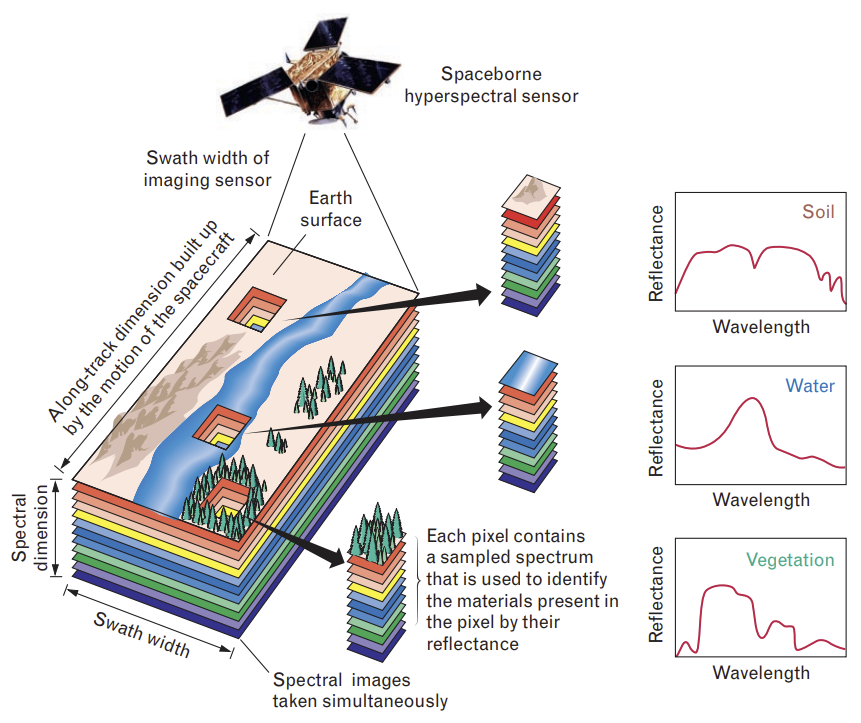
\includegraphics[width=0.6\textwidth]{media/hsi_remote_sensing.png}
	\caption{Schematic representation of a spaceborne hyperspectral imaging system used for remote sensing applications. \citep{hsi_remote_sensing}}
\end{figure}

However, the high dimensionality of hyperspectral data introduces the curse of dimensionality, leading to overfitting and reduced accuracy in classifiers. Moreover, the sheer volume of data increases computational cost and storage requirements. To address these issues, dimensionality reduction (DR) is commonly employed to extract compact, informative features that retain class-relevant information.

Among unsupervised DR methods, Principal Component Analysis (PCA) is widely used due to its simplicity and effectiveness. PCA finds orthogonal directions of maximum variance in the data and projects the high-dimensional data into a low-dimensional subspace. However, PCA operates solely in the spectral domain and does not take into account the spatial structure of hyperspectral images. Since neighboring pixels in HSIs are often part of the same class, ignoring spatial coherence can lead to poor low-dimensional representations. As a result, the features extracted by PCA may lack discriminative power and can be highly sensitive to noise.

To address the limitations, Jiang et al.\ \citep{SuperPCA} proposed the SuperPCA method, which leverages the idea that different regions in an image may require different linear projections for effective feature extraction. Specifically, the hyperspectral image is segmented into superpixels -- spatially contiguous regions with similar spectral characteristics -- and PCA is applied independently within each superpixel. This approach allows the model to capture local spectral--spatial structures by tailoring the dimensionality reduction to each region. SuperPCA has demonstrated higher classification accuracy compared to traditional spectral-only DR methods. However, it still relies solely on local information and ignores the global structures of HSIs, which leads to unsatisfactory performance in scenarios where superpixels contain mixed-class pixels or lack sufficient structure.


The Spectral–Spatial and Superpixelwise PCA (S3-PCA) method proposed by Zhang et al.\ \citep{S3PCA} improves upon SuperPCA by combining both global and local spectral–spatial information. It first performs local reconstruction within superpixels to enhance spatial consistency and reduce noise, and then applies PCA globally and locally to extract discriminative features at multiple scales. These features are concatenated to form a joint representation that better supports classification.

The goal of this project is to implement these superpixelization based PCA techniques for unsupervised feature extraction from hyperspectral images and evaluate their performance.



\section{Work Done Before Stage-1 Review} \label{sec:stage1}

\subsection{Theoretical Background}
  
As the first step of the project, an in-depth study of PCA, image segmentation techniques -- specifically Simple Linear Iterative Clustering (SLIC) \citep{SLIC} and Entropy Rate Superpixelization (ERS) \citep{ERS} algorithms -- and superpixel-based PCA methods was conducted.
\subsubsection{Principal Component Analysis (PCA)}

Given high-dimensional data \( X = \{x_1, x_2, \dots, x_P\} \in \mathbb{R}^{P \times B} \) with row-wise mean zero, where \( P \) is the number of samples and \( B \) is the feature dimensionality, Principal Component Analysis (PCA) aims to find a linear transformation that projects the data from the original \( B \)-dimensional feature space to a lower \( d \)-dimensional space \( Y = \{y_1, y_2, \dots, y_P\} \in \mathbb{R}^{P \times d} \), such that the projected data retains the maximum variance. The transformation is defined by a matrix \( W \in \mathbb{R}^{B \times d} \), and the linear projection is given by \( Y = XW\). The goal of PCA is to find the optimal projection matrix \( W \) that maximizes the variance of the projected data. This is achieved by solving the following optimization problem:
\begin{equation}
	W^* = \underset{W^T W = I}{\arg\max} \quad \text{Tr}(W^T \, \text{Cov}(X) \, W)
\end{equation}
where \(\text{Cov}(X)\) is the covariance matrix of the data and is given by 
\begin{equation}
	\text{Cov}(X) = \frac{1}{P} X^T X
\end{equation}


The matrix \( W \) is formed by selecting the eigenvectors corresponding to the \( d \) largest eigenvalues of \( \text{Cov}(X) \). These eigenvectors define the directions of maximum variance in the data.

PCA is widely used for dimensionality reduction in several applications due to its simplicity and computational efficiency. However, HSI data often exhibits spatial homogeneity -- nearby pixels are more likely to belong to the same class. Reshaping a 3D hyperspectral cube into a 2D matrix for PCA disregards this spatial structure, leading to suboptimal feature extraction.

\subsubsection{Entropy Rate Superpixelization (ERS)}\label{sec:ers}
The first step in any superpixel-based PCA method is the segmentation of the image into homogeneous clusters of pixels with similar spectral signatures. The goal of superpixelization is to partition the image into regions that exhibit spatial homogeneity, where each region contains pixels with similar properties. 

The Entropy Rate Superpixel (ERS) algorithm is a graph-based image segmentation method designed to generate compact and homogeneous superpixels. It formulates the superpixelization task as a graph partitioning problem, balancing two key objectives: preserving similarity within superpixels and maintaining spatial compactness.

The input image is represented as an undirected weighted graph \( G = (V, E) \), where:
\begin{itemize}
	\item Each vertex \( v_i \in V \) corresponds to a pixel.
	\item Each edge \( e_{ij} \in E \) connects neighboring pixels \( v_i \) and \( v_j \).
	\item Each edge is assigned a weight \( w_{ij} \), reflecting the similarity between the connected pixels, typically based on color or spectral features and spatial distance.
\end{itemize}

In this work, the weights for the edges between connected pixels are calculated using a Gaussian kernel. The similarity between two pixels, \(v_i\) and \(v_j\), is defined as:

\[
w_{ij} = \exp\left(- \frac{d(v_i, v_j)^2}{2\sigma^2}\right)
\]

where \(d(v_i, v_j)\) represents the distance between the pixels, computed as the intensity difference between their spectral features, multiplied by the spatial distance between them. Unlike the original work, which used a fixed kernel bandwidth, we adaptively choose the kernel bandwidth \(\sigma\) to be equal to the standard deviation of the norms of the spectral intensities of the image being segmented. This modification, which allows the bandwidth to vary with the characteristics of the image, showed better results in our experiments.

The goal of ERS is to select a subset of edges \( A \subseteq E \) such that the resulting graph partitions the image into \( K \) connected components (superpixels). The objective function maximizes the entropy rate of a random walk on the selected subgraph, while incorporating a balancing term that penalizes uneven superpixel sizes.

\begin{equation}
	\max_{A \subseteq E} \; \mathcal{F}(A) = H(A) + \lambda B(A)	
\end{equation}
where:
\begin{itemize}
	\item \( H(A) \) is the \textit{entropy rate} term encouraging similarity within superpixels.
	\item \( B(A) \) is the \textit{balancing term} promoting superpixels of similar size.
	\item \( \lambda \) is a regularization parameter balancing the two terms.
\end{itemize}

\paragraph{Entropy Rate Term \( H(A) \):}

Let \( \pi_i \) denote the stationary distribution of a random walk at node \( v_i \) (i.e., the long-run probability of visiting node \( v_i \) if the walk continues indefinitely), and \( p_{ij} \) be the transition probability from \( v_i \) to \( v_j \). The entropy rate of the random walk is given by:

\begin{equation}
	H(A) = - \sum_{i \in V} \pi_i \sum_{j \in V} p_{ij} \log p_{ij}
\end{equation}

with transition probabilities defined as:

\begin{equation}
	p_{ij} = \frac{w_{ij}}{w_i}, \quad \text{where } w_i = \sum_{k:e_{ik} \in E} w_{ik}
\end{equation}


and the stationary distribution:

\begin{equation}
\pi_i = \frac{w_i}{\sum_{k \in V} w_k}
\end{equation}

This term encourages edge selections that preserve strong similarities between connected nodes, resulting in homogeneous superpixels.

\paragraph{Balancing Term \( B(A) \):}

Let \( A \) be the selected edge set, \( N_A \) the number of connected components (superpixels), and \( Z_A \) the distribution of cluster memberships. The distribution \( p_{Z_A}(i) \) is:

\begin{equation}
	p_{Z_A}(i) = \frac{|S_i|}{|V|}, \quad i = 1, \dots, N_A
\end{equation}

where \( S_i \) denotes the set of vertices (pixels) that belong to the \( i \)-th superpixel or connected component after the graph partitioning.

The balancing term is defined as:

\begin{equation}
	B(A) = - \sum_{i=1}^{N_A} p_{Z_A}(i) \log(p_{Z_A}(i)) - N_A
\end{equation}

where \( H(Z_A) \) is the entropy function that favors clusters with similar sizes, and the term \( N_A \) penalizes a large number of clusters.

The ERS formulation results in a combinatorial optimization problem, which is solved using a greedy algorithm. The algorithm iteratively adds edges with the highest marginal gain until the number of connected components becomes \( K \). 

\subsubsection{Simple Linear Iterative Clustering (SLIC)}\label{sec:slic}

SLIC is a k-means like clustering algorithm that generates compact and nearly uniform superpixels by jointly considering color similarity and spatial proximity. It takes as input the desired number of superpixels \( K \), resulting in an approximate superpixel size of \( S^2 \), where \( S = \sqrt{N/K} \) for an image with \( N \) pixels. It uses a combined distance measure given by: 

\begin{equation}
	D_s = d_{lab} + \frac{m}{S}d_{xy}
\end{equation}

where \( d_{lab}\) is the euclidean distance in the \(lab\) color space and \(d_{xy}\) is the euclidean distance measuring spatial proximity. The hyperparameter \(m\) controls the compactness of the clusters, with higher values yielding more regularly shaped superpixels.

Clustering is performed similarly to the \(k\)-means algorithm in a joint five-dimensional space using the above distance measure. \( K \) regularly space cluster centers are initialized and each pixel is assigned to the nearest cluster center. After assignment, cluster centers are updated as the average of their assigned pixels. This process of assignment and update is repeated until convergence, typically in a few iterations. Although spatial proximity is encouraged during clustering, disconnected components can occasionally arise. A final post-processing step ensures spatial connectivity by relabeling small isolated regions to match neighboring segments.

Due to its conceptual simplicity, efficiency, and ease of implementation, SLIC has become one of the most widely used superpixelization algorithms and is readily available in popular libraries such as \texttt{scikit-image}.

\subsubsection{Superpixelwise Principal Component Analysis (SuperPCA)}\label{sec:spca}

Let \( \mathcal{X} \in \mathbb{R}^{M \times N \times B} \) denote an HSI, where \( M \), \( N \), and \( B \) are the spatial height, width, and number of spectral bands, respectively. The HSI is typically reshaped into a 2D matrix \( \mathbf{X} = [\mathbf{x}_1, \mathbf{x}_2, \dots, \mathbf{x}_P]^T \in \mathbb{R}^{P \times B} \), with \( P = MN \), and \( \mathbf{x}_i \in \mathbb{R}^B \) representing the spectral vector of a pixel.

\begin{figure}
	\centering
	
\includegraphics[width = 0.8\textwidth]{media/SuperPCA.png}
	\caption{Schematic of SuperPCA based dimensionality reduction for HSIs \citep{SuperPCA}.}
	\label{fig:superpca}
\end{figure}

In SuperPCA, dimensionality reduction is performed locally on spectrally homogeneous regions rather than globally. First, PCA is applied to the original HSI to obtain its first principal component, which captures the dominant spectral structure. This projection is used for superpixel segmentation of the image; the authors use Entropy Rate Superpixel Segmentation (ERS) for this purpose.

Each resulting superpixel defines a homogeneous region whose pixel spectra are collected into a matrix. PCA is then applied independently to each of these regional matrices to learn intrinsic low-dimensional features. Finally, the reduced representations from all regions are reorganized and merged to reconstruct a low-dimensional version of the HSI, as illustrated in Figure~\ref{fig:superpca}.

\subsubsection{Spectral-Spatial-Superpixelwise Principal Component Analysis (S3-PCA)}\label{sec:s3pca}

S3-PCA uses the same method as SuperPCA to segment the HSI into multiple homogeneous regions using ERS. After segmentation, a spatial reconstruction step is performed to denoise the HSI. In each homogeneous region, every pixel $\mathbf{x}_i \in \mathbb{R}^B$ is reconstructed using its $k$ nearest spatial neighbors $\{\mathbf{z}_1, \dots, \mathbf{z}_k\}$ within the same superpixel. The similarity between $\mathbf{x}_i$ and each neighbor $\mathbf{z}_j$ is computed using a Gaussian-weighted scheme:

\begin{equation}
	w_j = \left. \exp \left( - \frac{\| \mathbf{x}_i - \mathbf{z}_j \|_2^2}{2t^2} \right) \right/ h, \quad
	t = \frac{1}{k} \sum_{j=1}^{k} \| \mathbf{x}_i - \mathbf{z}_j \|_2^2, \quad
	h = \sum_{j=1}^{k} \exp \left( - \frac{\| \mathbf{x}_i - \mathbf{z}_j \|_2^2}{2t^2} \right)
\end{equation}

and the reconstructed pixel is given by:

\begin{equation}
	\mathbf{x}_i^* = \sum_{j=1}^{k} w_j \mathbf{z}_j.
\end{equation}

Once all pixels are reconstructed, PCA is applied to each superpixel region to extract local low-dimensional spectral--spatial features. To further capture global structure, PCA is also applied to the reconstructed HSI as a whole, yielding global features. The local and global features are then concatenated, and a final round of PCA is applied to reduce the dimensionality of the combined feature set.

\begin{figure}
	\centering
	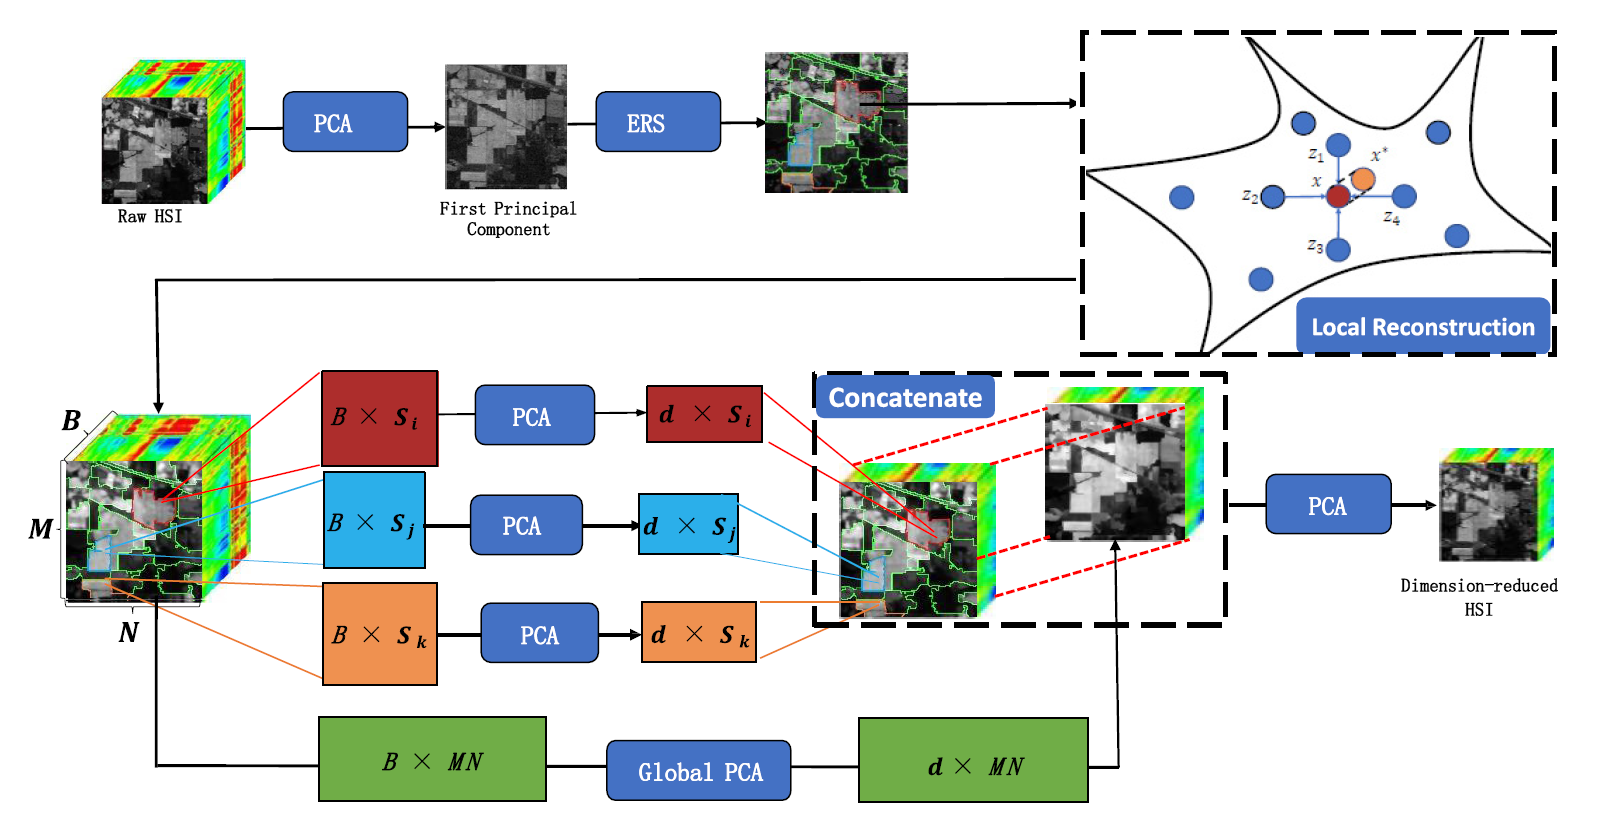
\includegraphics[width = 0.9\textwidth]{media/S3-PCA.png}
	\caption{Schematic of S3-PCA based dimensionality reduction for HSIs \citep{S3PCA}.}
	\label{fig:s3pcaa}
\end{figure}

\subsection{Partial Implementation and Preliminary Results}
As part of the initial work, a framework for performing SuperPCA and S3-PCA was developed in Python. For image segmentation, the SLIC algorithm from the \texttt{scikit-image} library was used. Preliminary classification results were obtained on the Indian Pines HSI dataset.

The Indian Pines scene consists of $145 \times 145$ pixels and 220 spectral bands ranging from 0.4 to 2.45~$\mu$m, capturing agricultural land with a regular geometric structure. In accordance with common preprocessing practices, 20 low signal-to-noise ratio (SNR) bands were removed, resulting in 200 usable bands. The dataset includes 16 different land cover classes and provides ground-truth labels for approximately 10,249 pixels. This dataset is publicly available at the \textit{Hyperspectral Remote Sensing Scenes} repository maintained by the Grupo de Inteligencia Computacional (GIC)\footnote{\url{http://www.ehu.eus/ccwintco/index.php?title=Hyperspectral_Remote_Sensing_Scenes}}.

The SuperPCA implementation includes a hyperparameter $S$, denoting the number of superpixels. For the preliminary results, $S = 97$ was used. In the case of S3-PCA, an additional parameter $k = 15$ was used, specifying the number of nearest spatial neighbors in the reconstruction step. These values were chosen based on those found to be optimal in the original study \citep{SuperPCA, S3PCA}. 

Dimensionality reduction was performed using SuperPCA and S3-PCA, reducing the hyperspectral data to $d = 30$ features, following the original methodology~\citep{SuperPCA, S3PCA}. After dimensionality reduction, $T = 30$ labeled samples per class were randomly selected as training data. Classification was performed using a kernel SVM with an RBF kernel, where the kernel parameters were selected through cross-validation. To ensure robustness, the training and classification steps were repeated 10 times with different random splits. The mean overall accuracy (OA) across these runs was reported. The results of the initial implementation, including classification maps, are shown in Figure~\ref{fig:preliminary_results}.

\begin{figure}[h!]
	\centering
	\begin{subfigure}[b]{0.24\textwidth}
		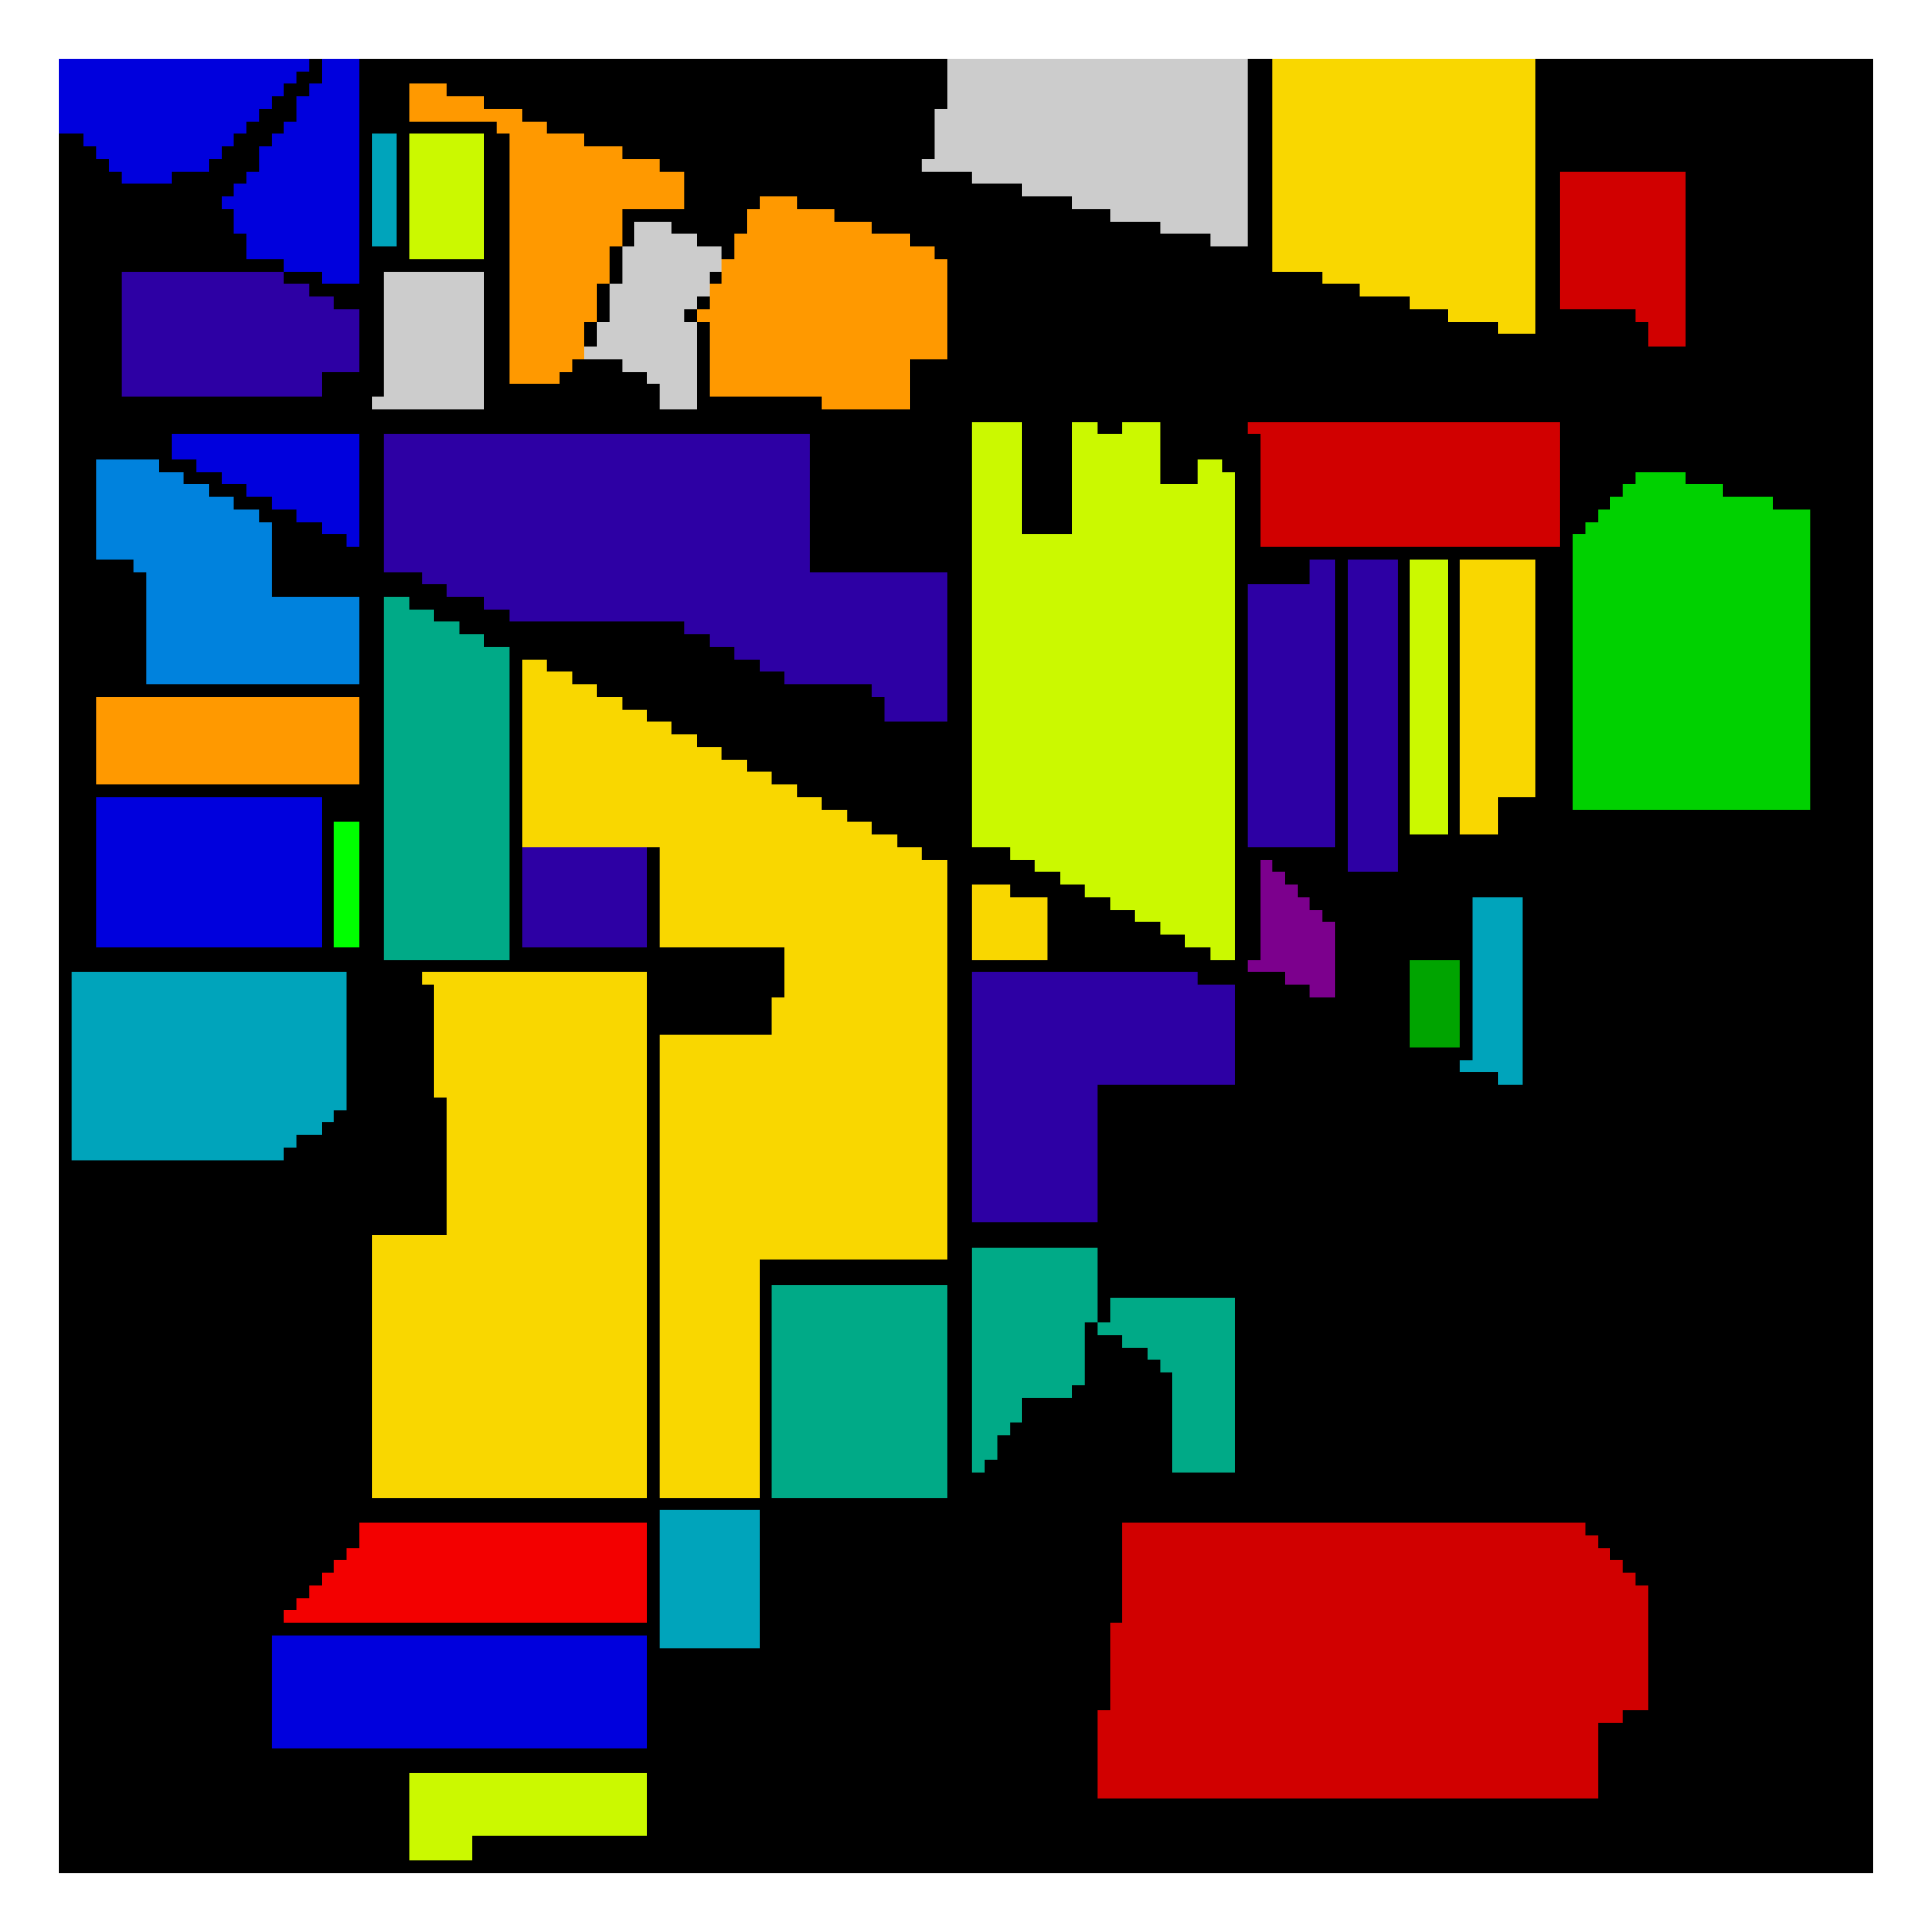
\includegraphics[width=\textwidth]{media/GroundTruth.png}
		\caption{}
	\end{subfigure}
	\begin{subfigure}[b]{0.24\textwidth}
		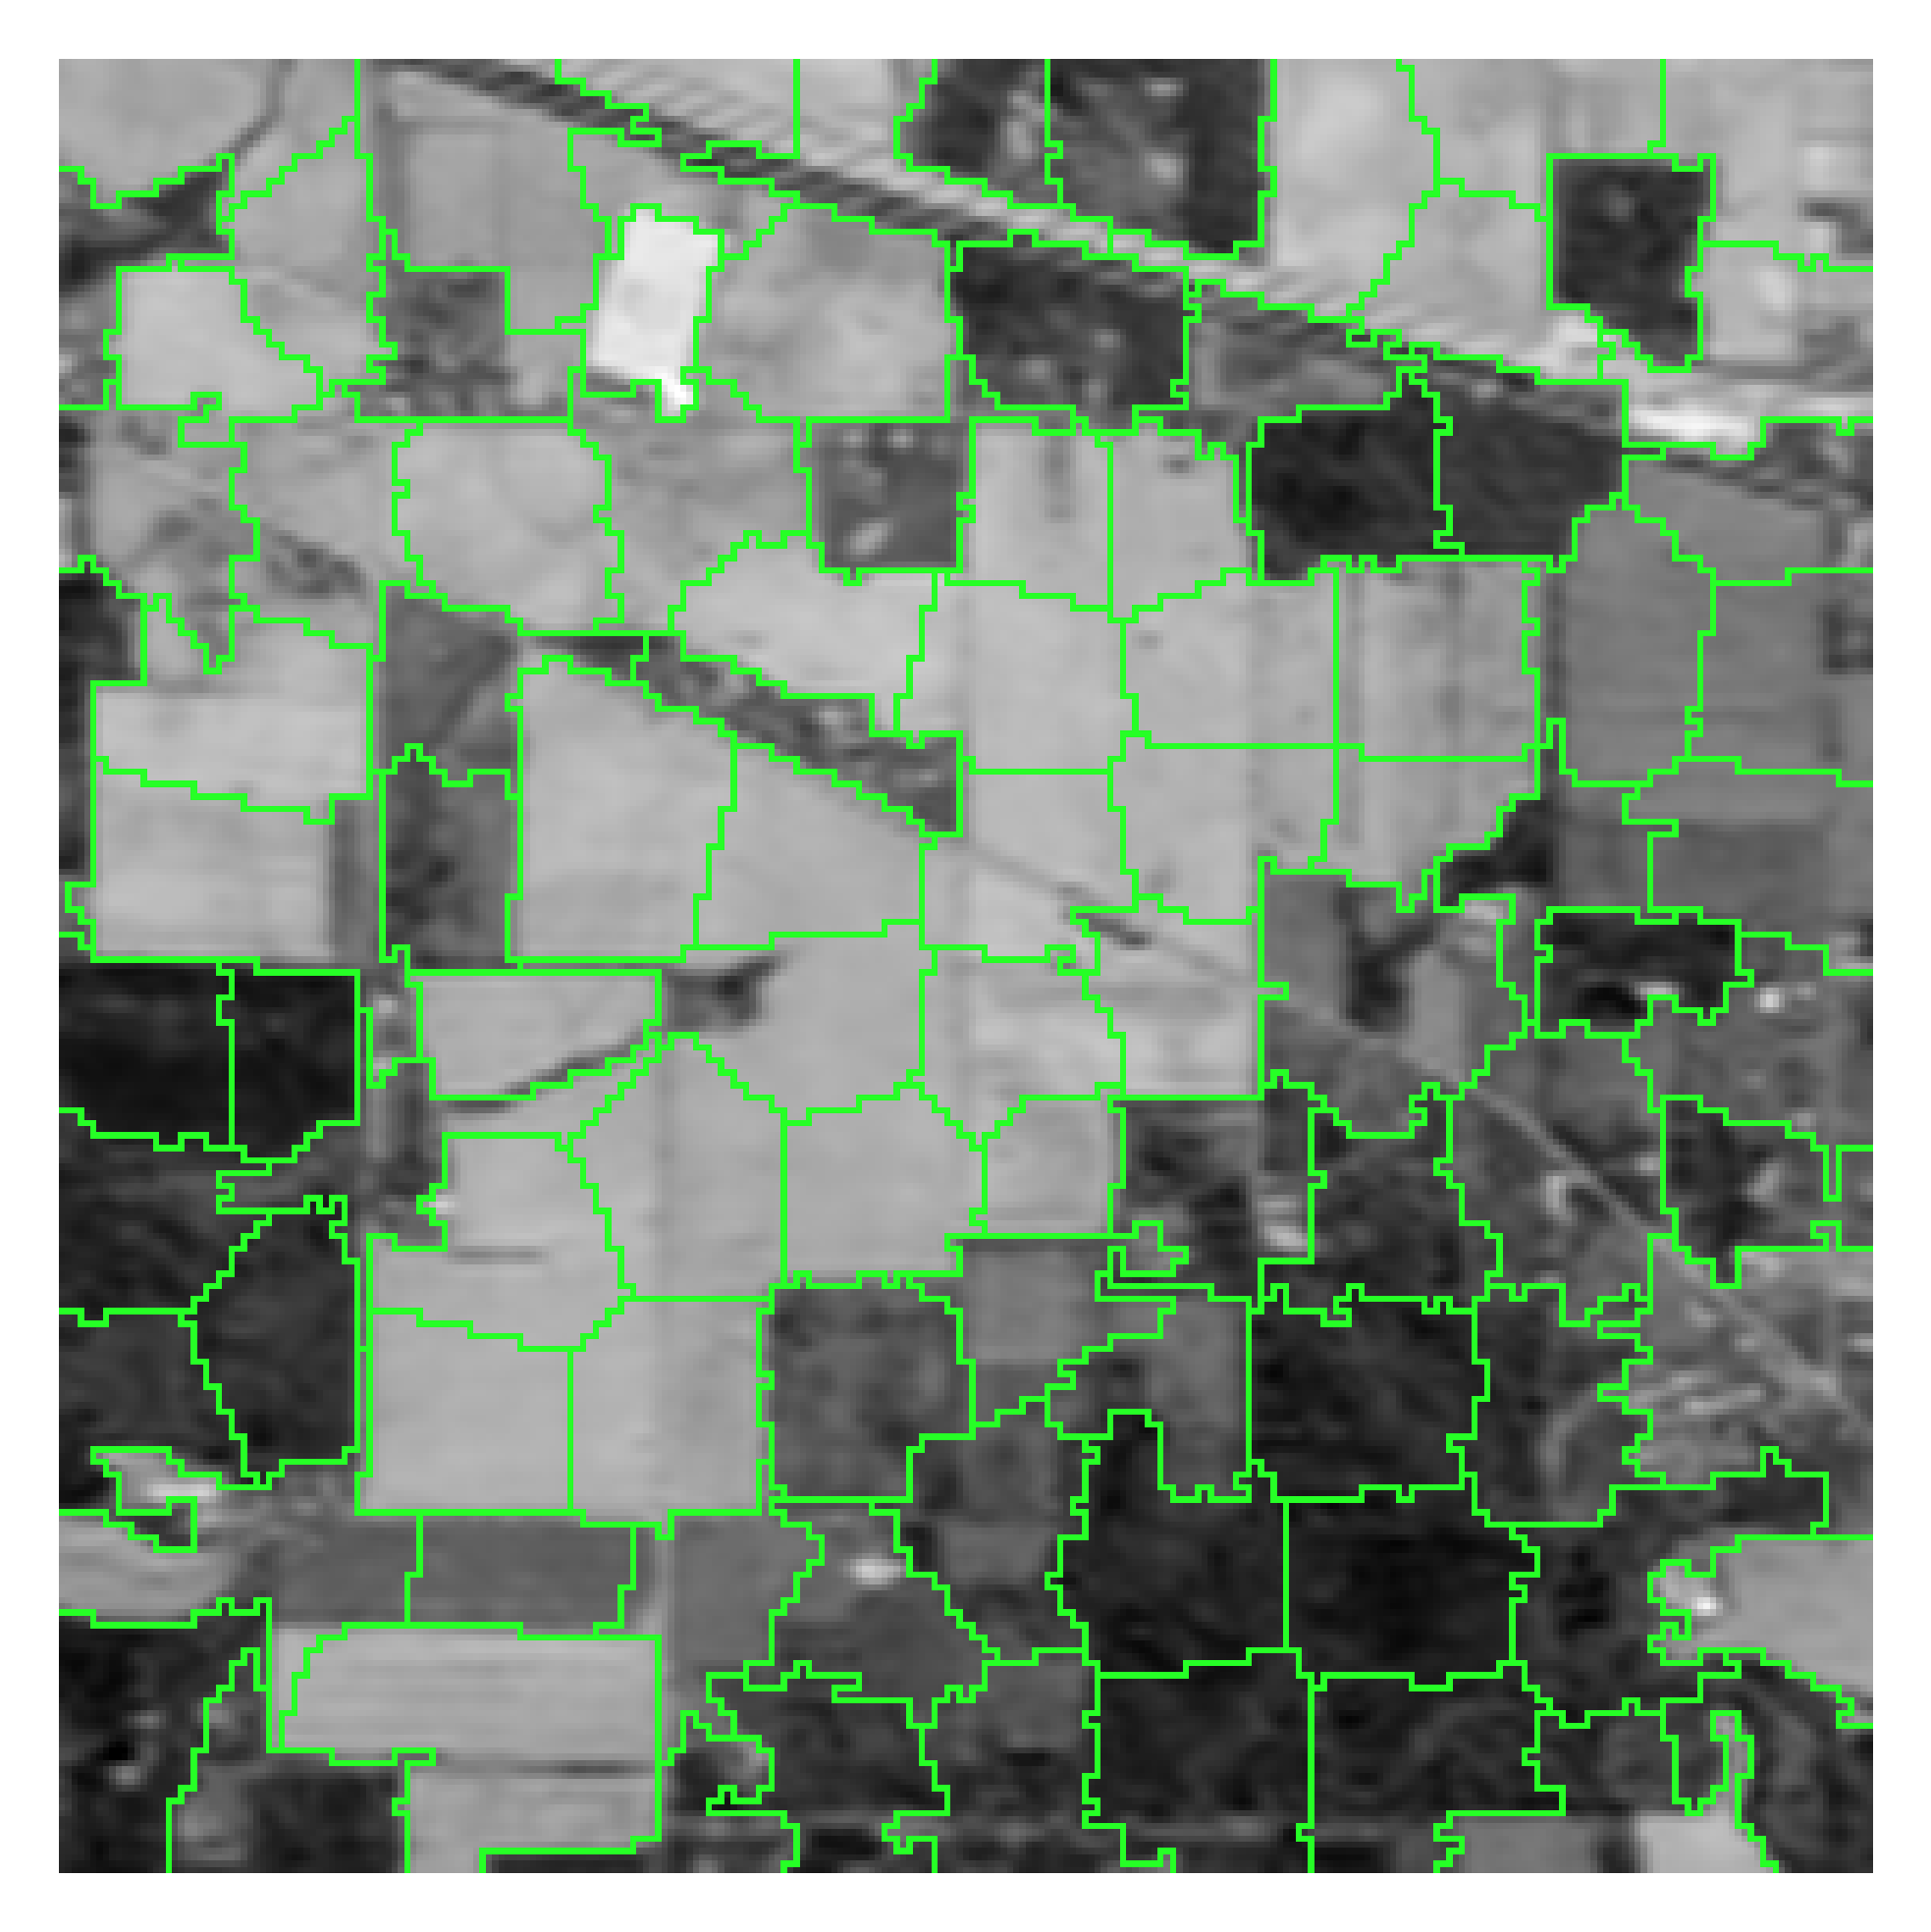
\includegraphics[width=\textwidth]{media/prelim_seg_img.png}
		\caption{}
	\end{subfigure}
	\begin{subfigure}[b]{0.24\textwidth}
		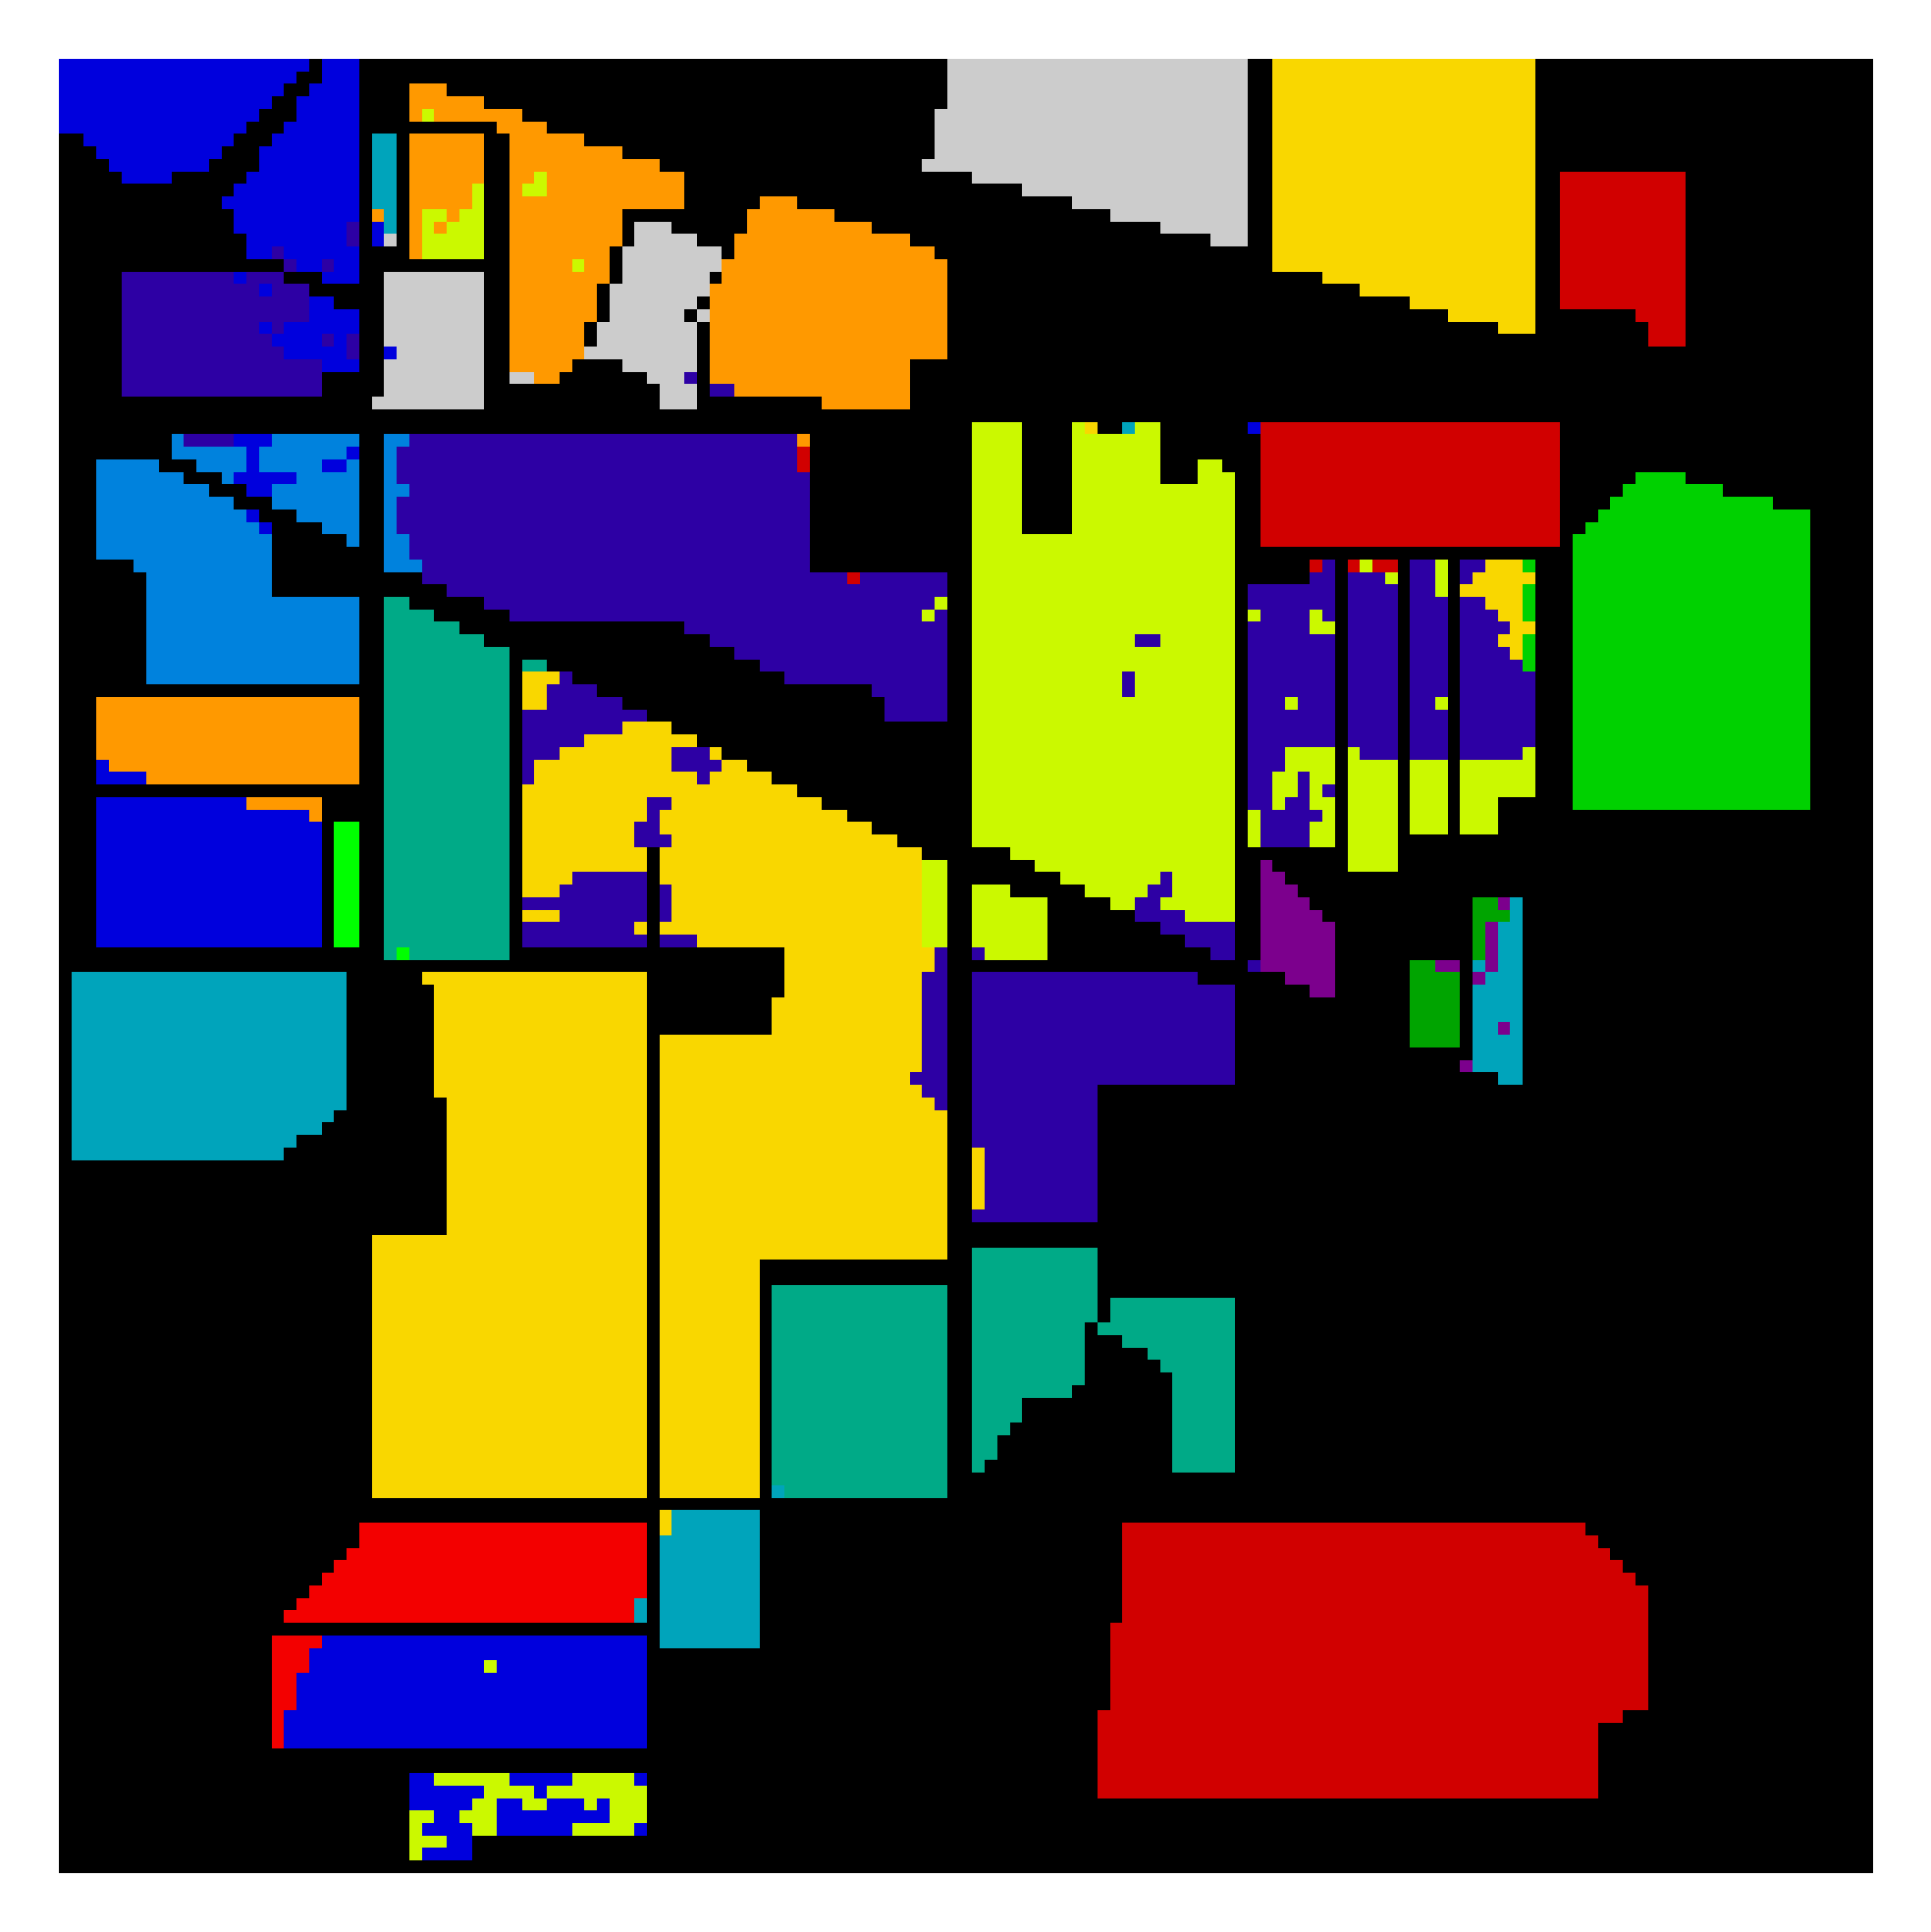
\includegraphics[width=\textwidth]{media/prelim_superpca_class_map.png}
		\caption{OA = 89.20\%}
	\end{subfigure}
	\begin{subfigure}[b]{0.24\textwidth}
		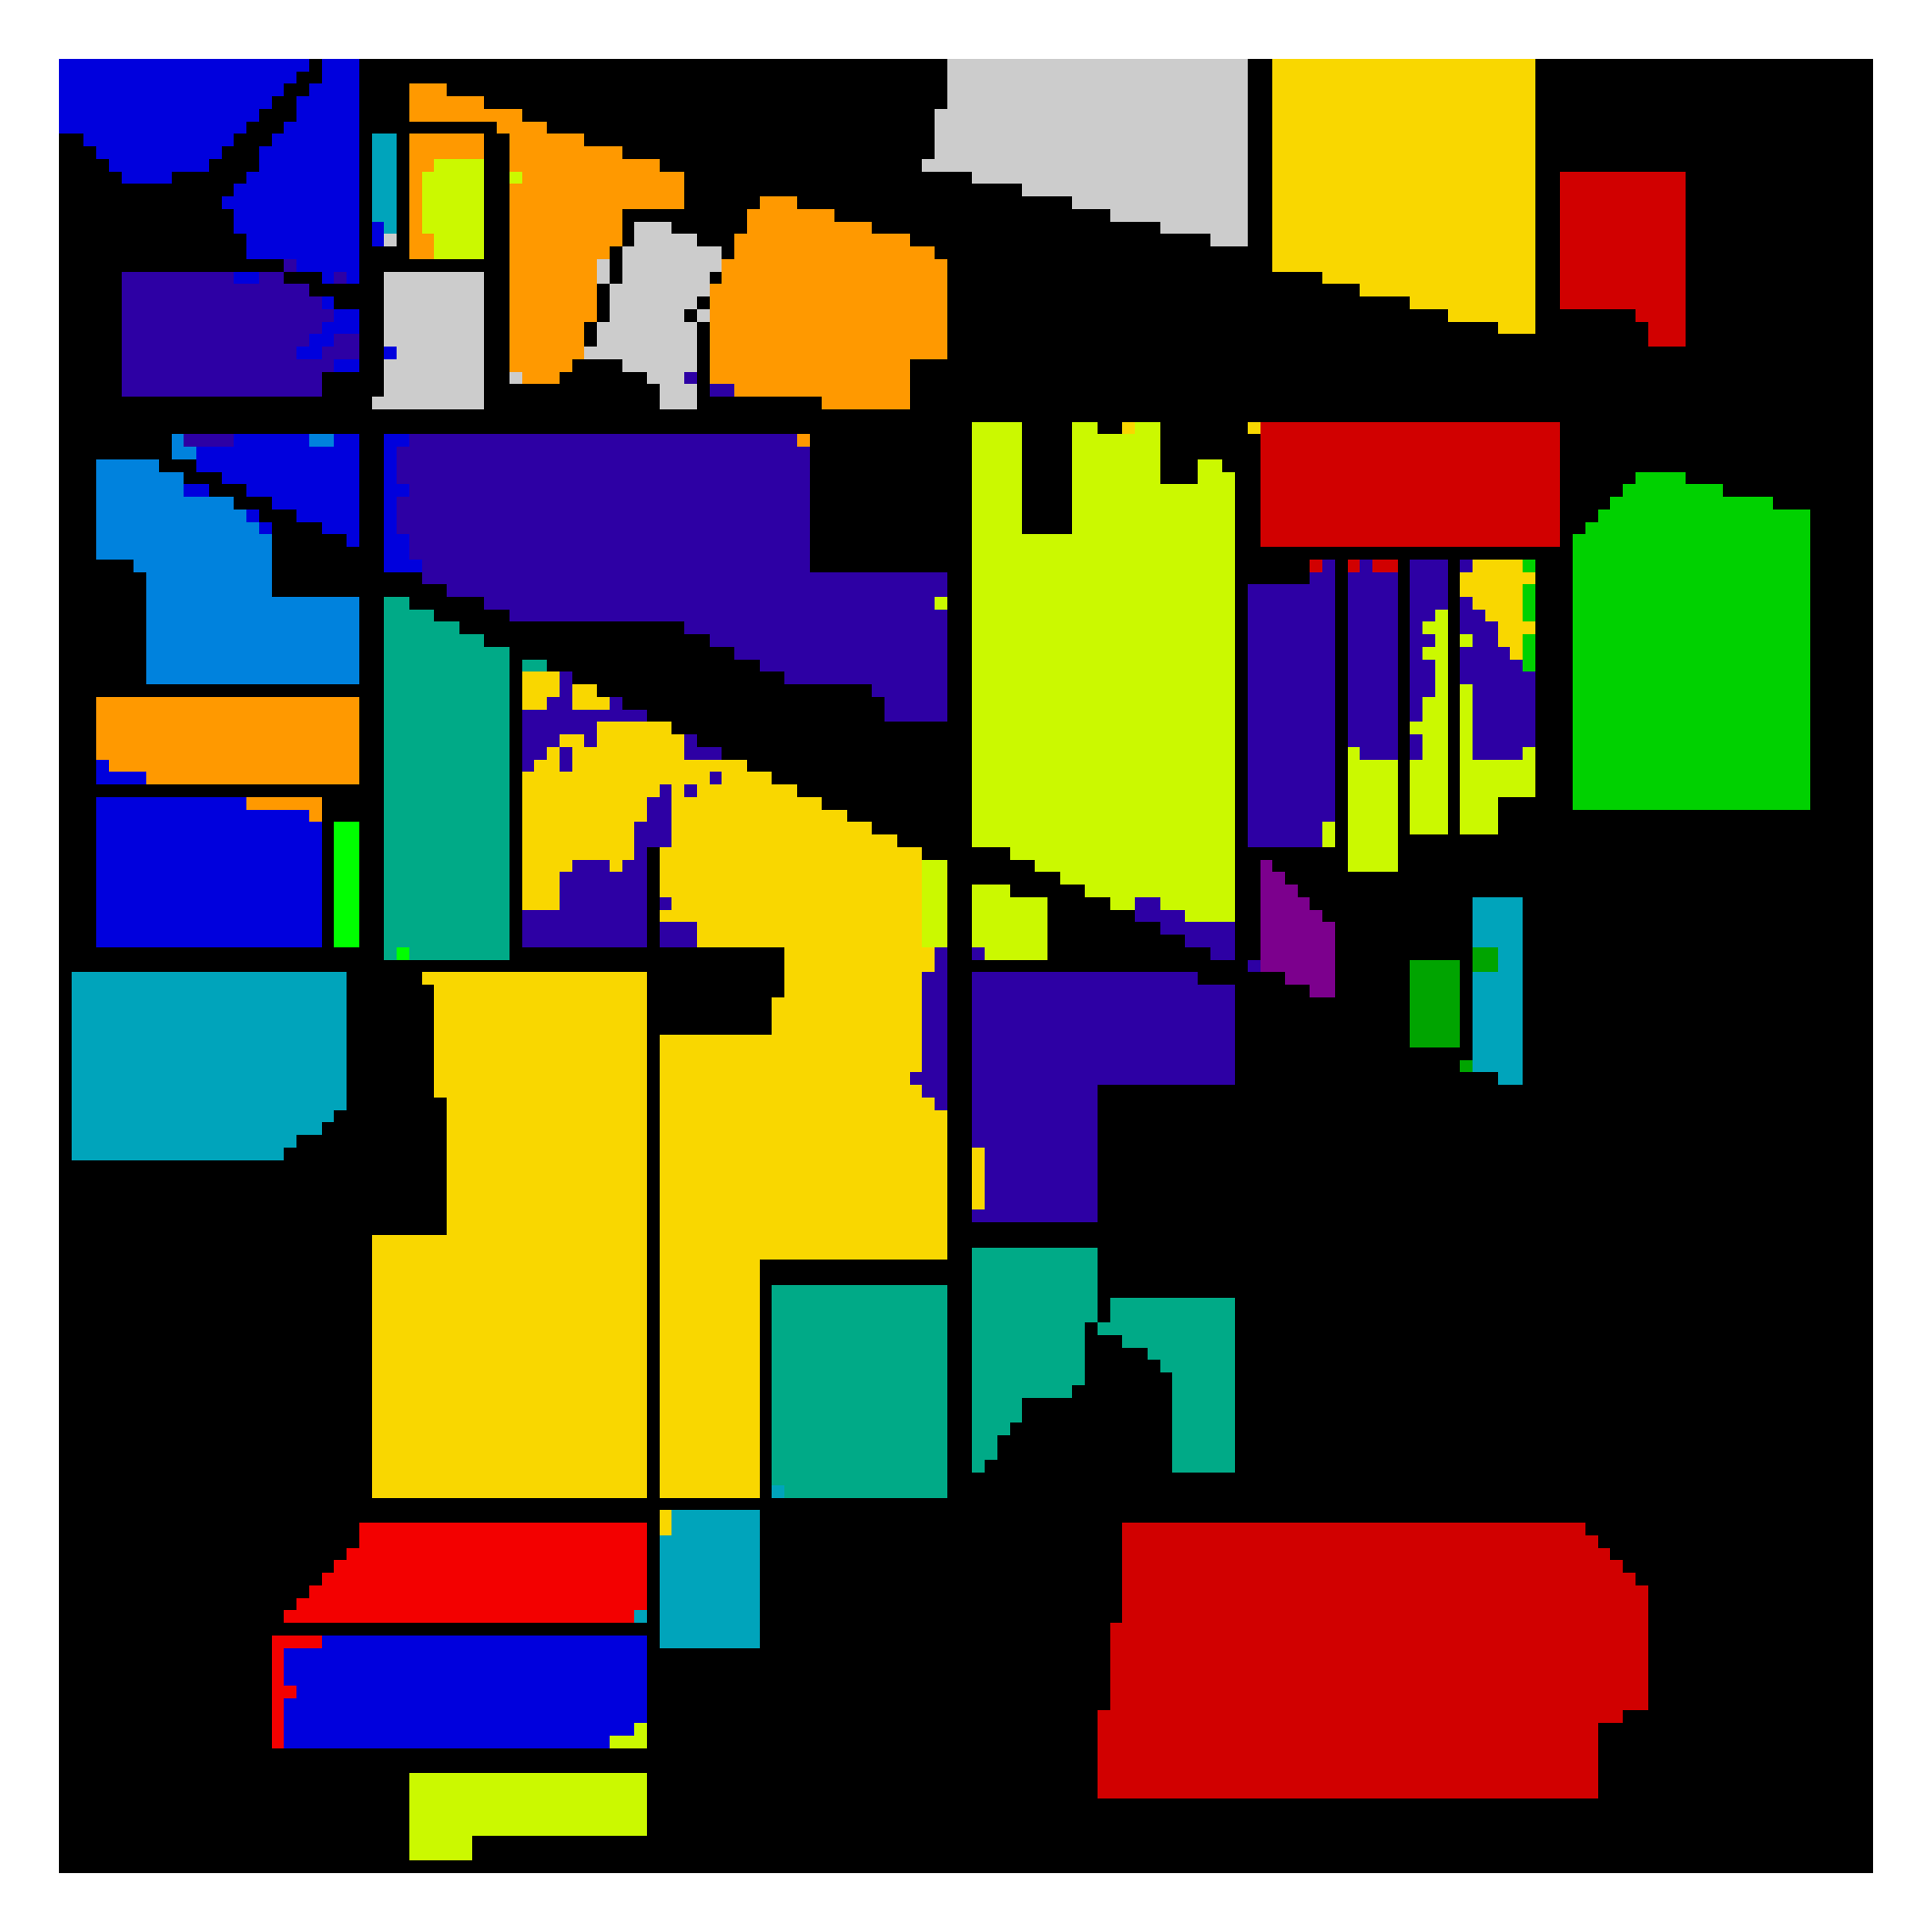
\includegraphics[width=\textwidth]{media/prelim_s3pca_class_map.png}
		\caption{OA = 90.30\%}
	\end{subfigure}
	\caption{Preliminary classification maps obtained with the Indian Pines dataset. (a) Ground truth, (b) First PCA projection along with segment boundaries obtained using SLIC, (c) SuperPCA, (d) S3-PCA.}
	\label{fig:preliminary_results}
\end{figure}

\section{Comments/Inputs given during the Stage-1 Review} \label{sec:stage1_comments}

During the Stage 1 review, it was recommended to continue with the ongoing experiments and build upon the preliminary results obtained so far. Additionally, it was emphasized that the ERS algorithm should be implemented from scratch in Python, as there is no publicly available implementation. Furthermore, a comparison between the results obtained from the SLIC algorithm and those from the ERS algorithm was suggested. This would help assess the effectiveness and accuracy of the ERS segmentation compared to the more commonly used SLIC method. Lastly, the review encouraged exploring potential modifications to improve the current method and boost overall performance.

\subsection{Addressing Comments after Stage-1 Review}
In response to the feedback provided during the Stage-1 review, several measures have been taken to address the comments and improve the progress of the project. First, the ERS algorithm was implemented using the greedy approach outlined in the original paper. The experiments from the paper were successfully replicated, and the algorithm was used to find optimal hyperparameters and evaluate its performance. Additionally, further experiments were conducted to compare the results from ERS with those obtained from the SLIC algorithm.

Two new approaches were explored to improve the methodology. The first approach involved using the full HSI data for segmentation, rather than just the first principal component, which was previously used. This adjustment was made possible with the ERS algorithm, as it supports segmentation of the full HSI, unlike SLIC in scikit-image, which only accepts grayscale or RGB images. The second approach modified the reconstruction process, where instead of relying solely on spectral similarity to calculate reconstruction weights, spatial proximity was incorporated to weigh the neighboring pixels.

\section{Experiments and Replications of Algorithms in Paper} 
All experiments in this work have been conducted on the Indian Pines hyperspectral dataset. The other datasets used in the original paper are more than ten times larger in size, making it computationally infeasible to process them with the available resources.

The experimental pipeline closely follows the methodology outlined in the original SuperPCA paper. First, we perform parameter tuning for the SuperPCA and S3-PCA methods to identify optimal values for the number of superpixels ($S$) and the number of neighbors ($k$) used in the reconstruction step. Subsequently, we compare the classification performance of PCA, SuperPCA, and S3-PCA, and demonstrate the effectiveness of the superpixelization based methods over conventional PCA.

\subsection{Parameter Tuning}\label{sec:parametertuning}

We first investigate the influence of the number of superpixels on the performance of the SuperPCA method. Dimensionality reduction is performed with SuperPCA using $S = \{1, 3, 5, 10, 20, 30, 40, 50, 75, 100, 150, 200, 300\}$ superpixels. SVM classification is then carried out with $T = \{5, 10, 20, 30\}$ training samples per class. For classes with fewer samples, only half of the total available samples are used. Figure~\ref{fig:exp1} shows the results of this exercise.

The results show that overall accuracy initially increases with $S$, but then declines when $S$ becomes too large. A small number of superpixels leads to under-segmentation, mixing samples from different homogeneous regions. Conversely, too many superpixels result in over-segmentation and reduce the sample size within each region, negatively affecting PCA stability. For the Indian Pines dataset, an optimal performance is achieved when $S = 50$.

\begin{figure}[h!]
	\centering
	\begin{subfigure}[b]{0.4\textwidth}
		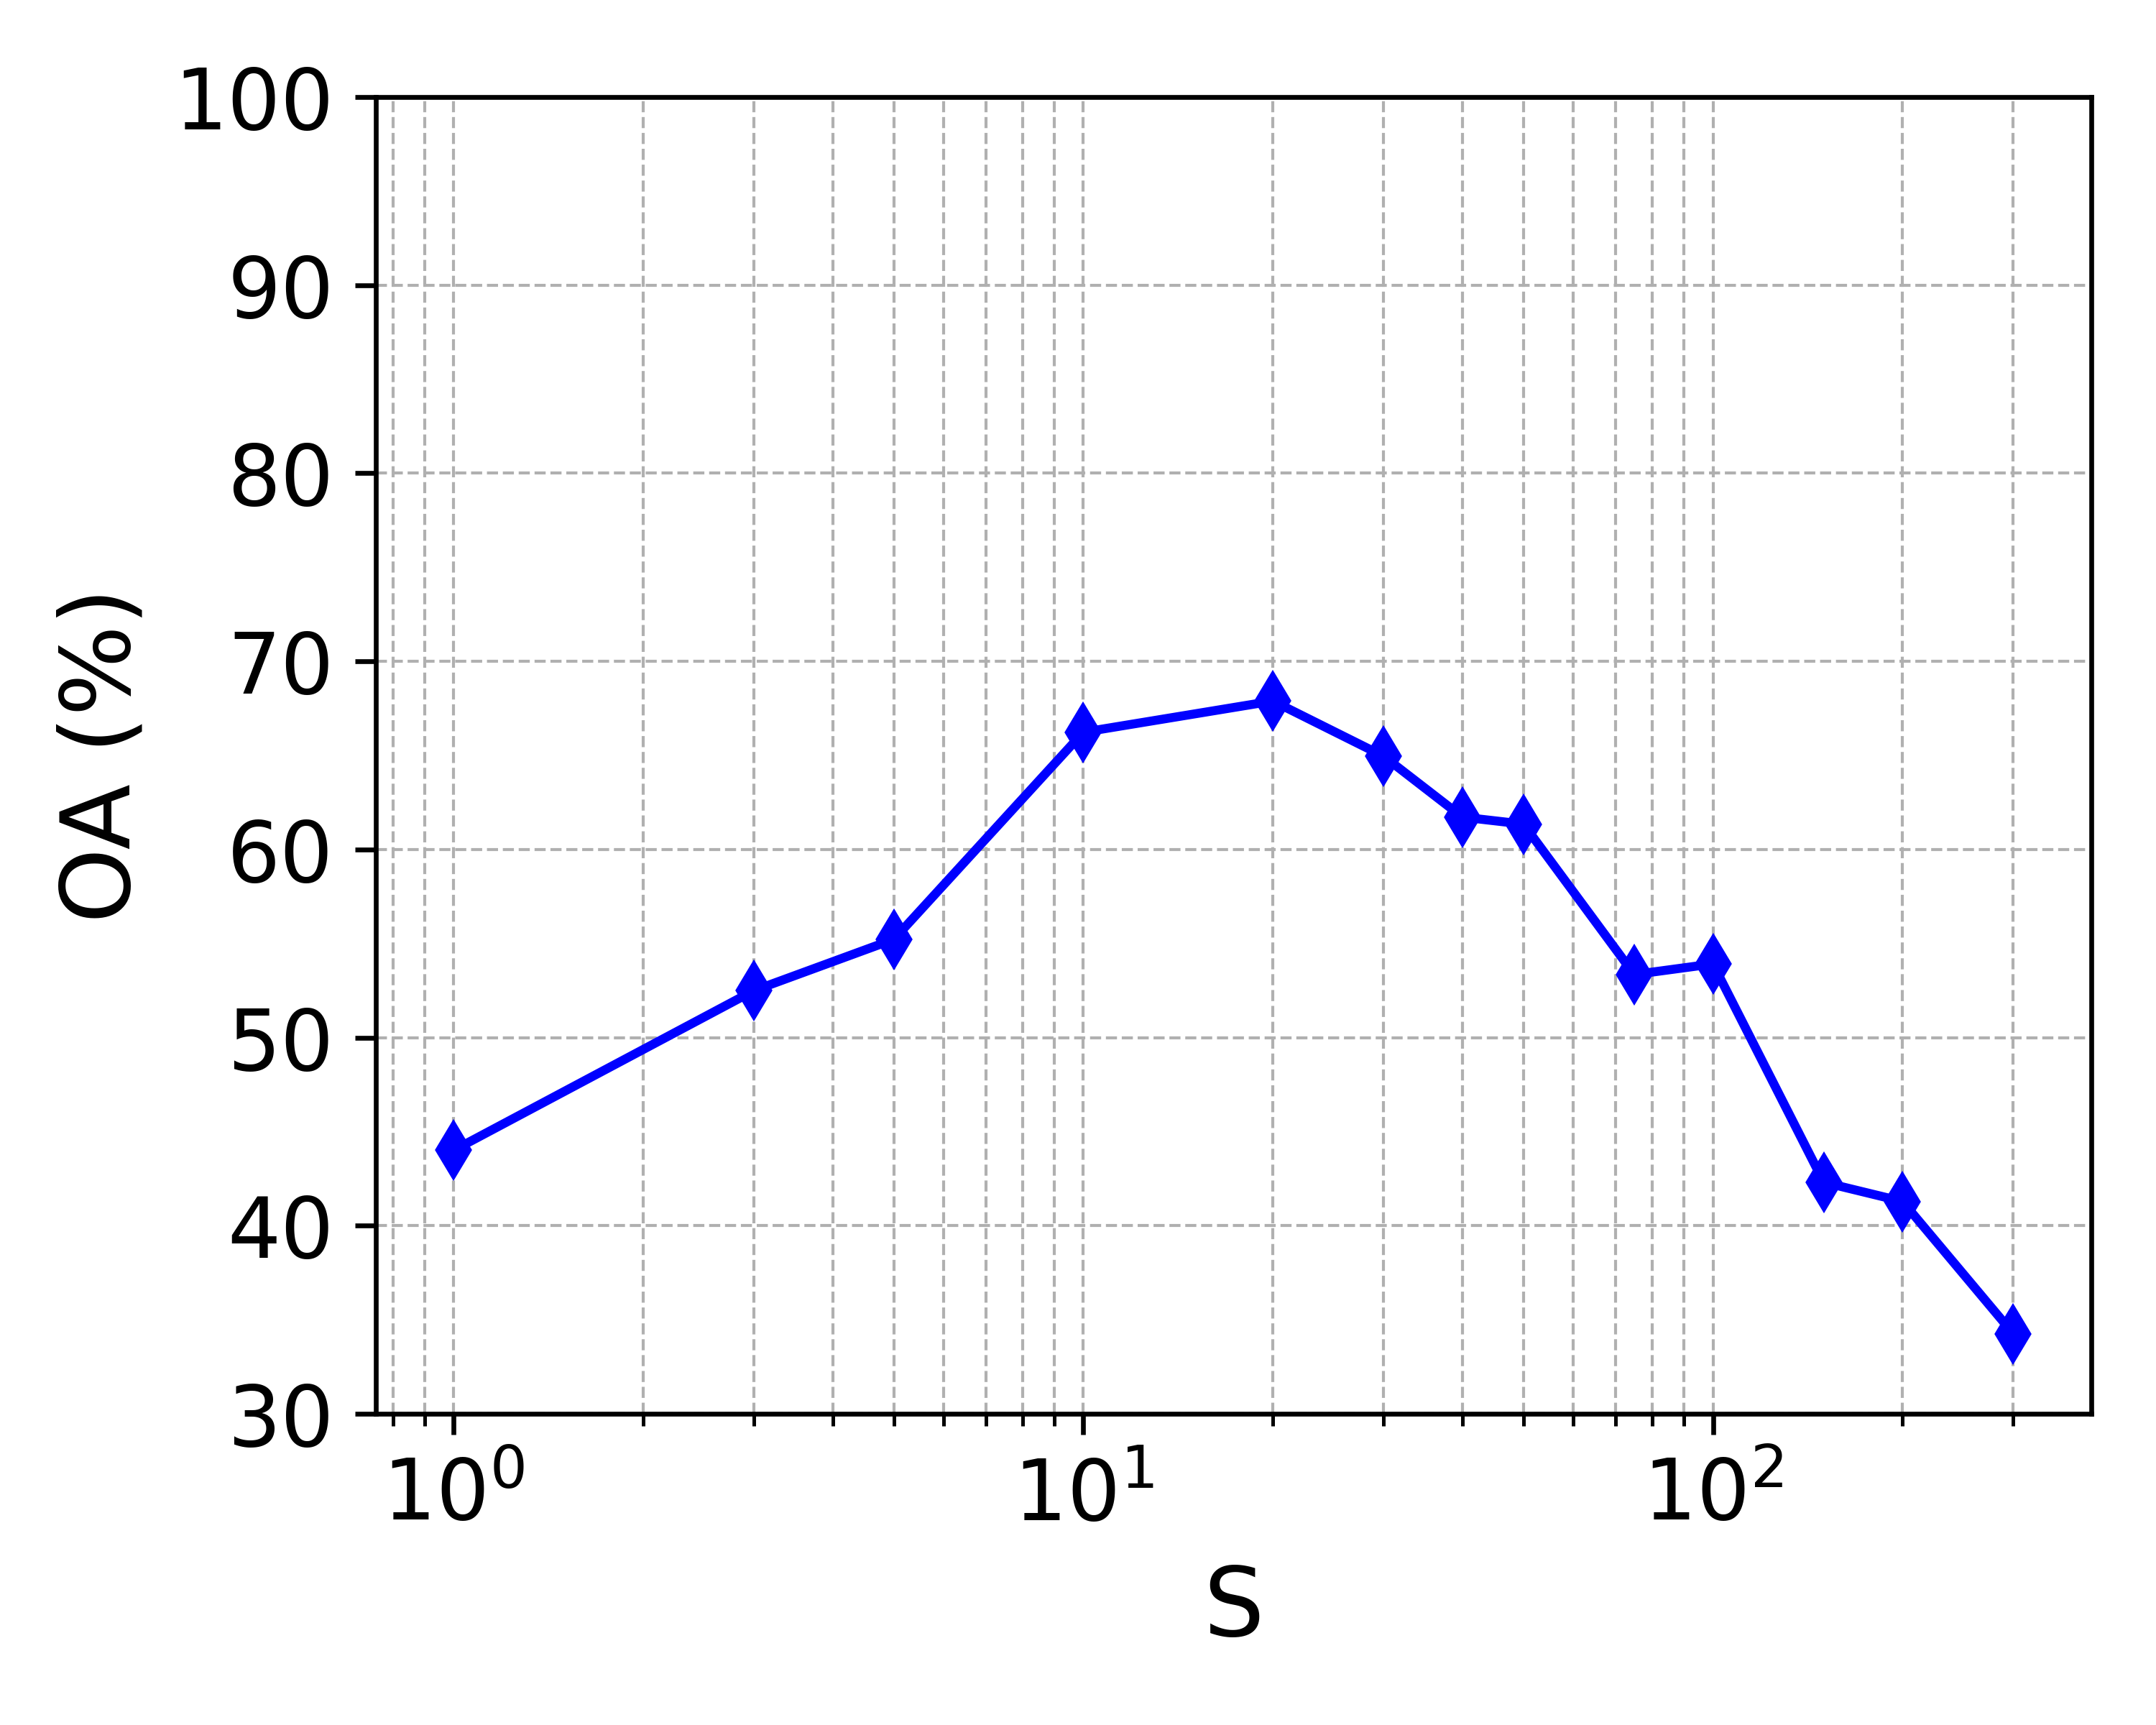
\includegraphics[width=\textwidth]{media/Exp1_T_5.png}
		\caption{}
	\end{subfigure}
	\begin{subfigure}[b]{0.4\textwidth}
		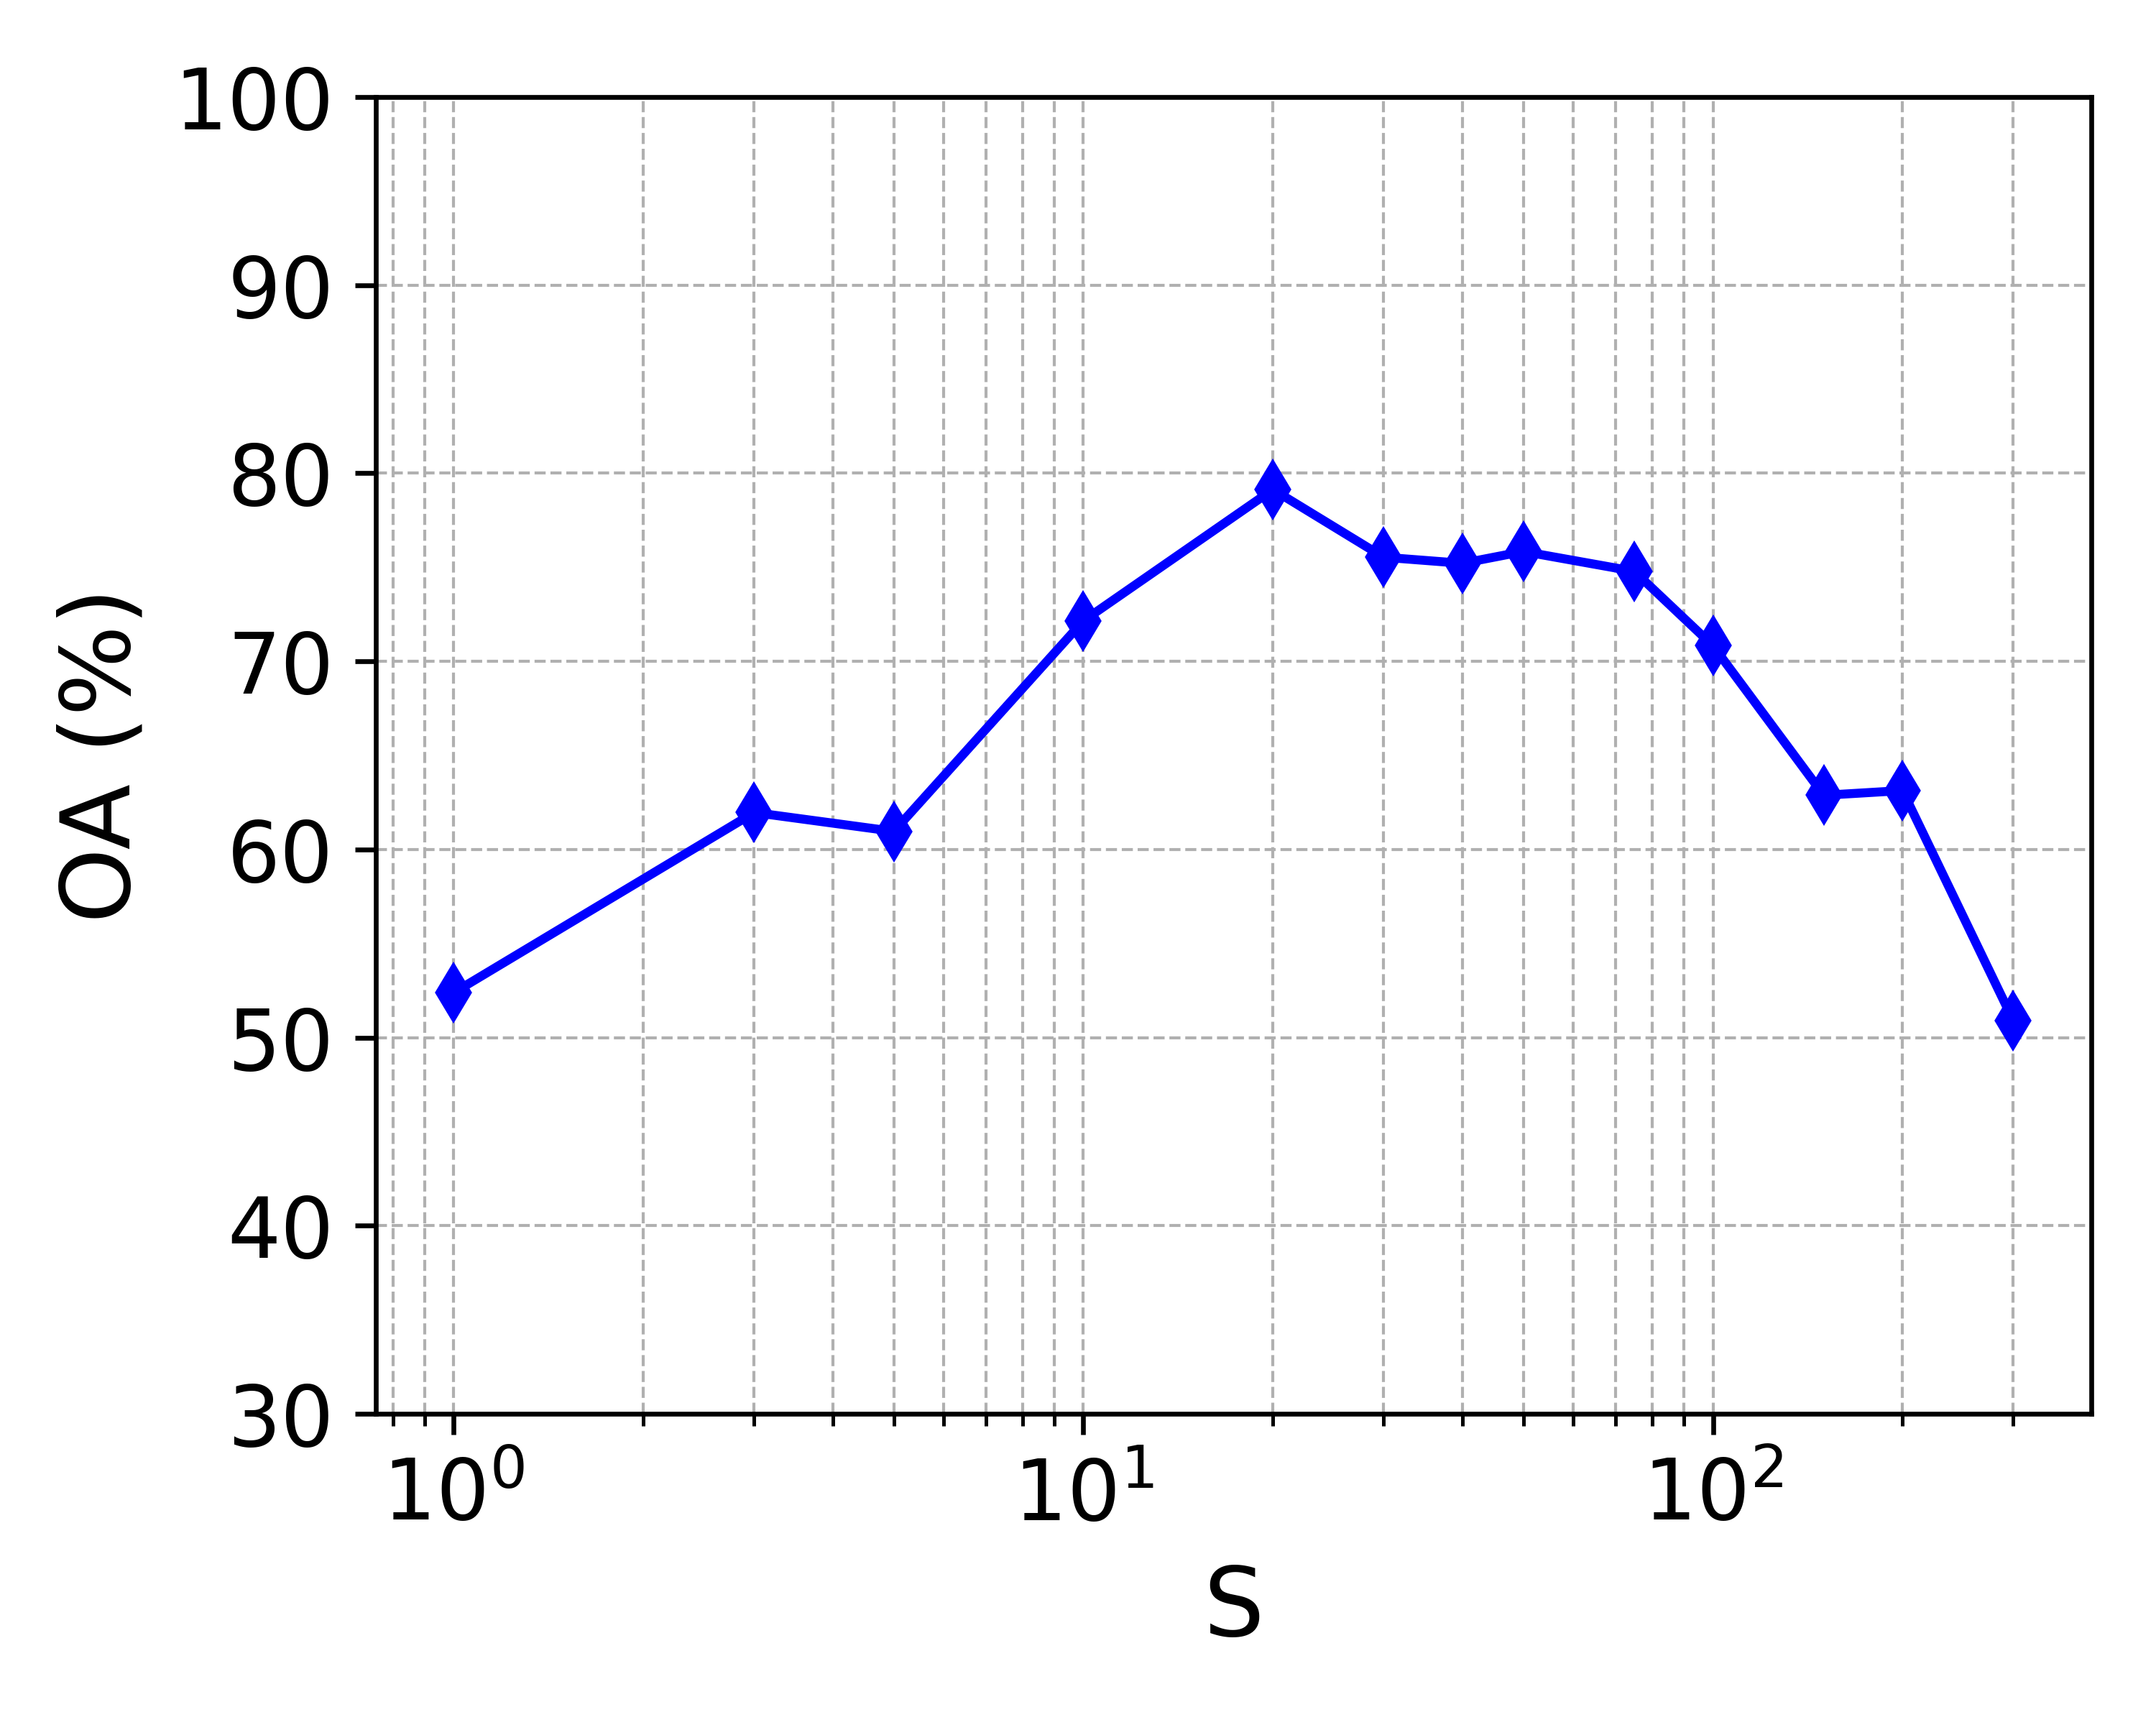
\includegraphics[width=\textwidth]{media/Exp1_T_10.png}
		\caption{}
	\end{subfigure}
	\begin{subfigure}[b]{0.4\textwidth}
		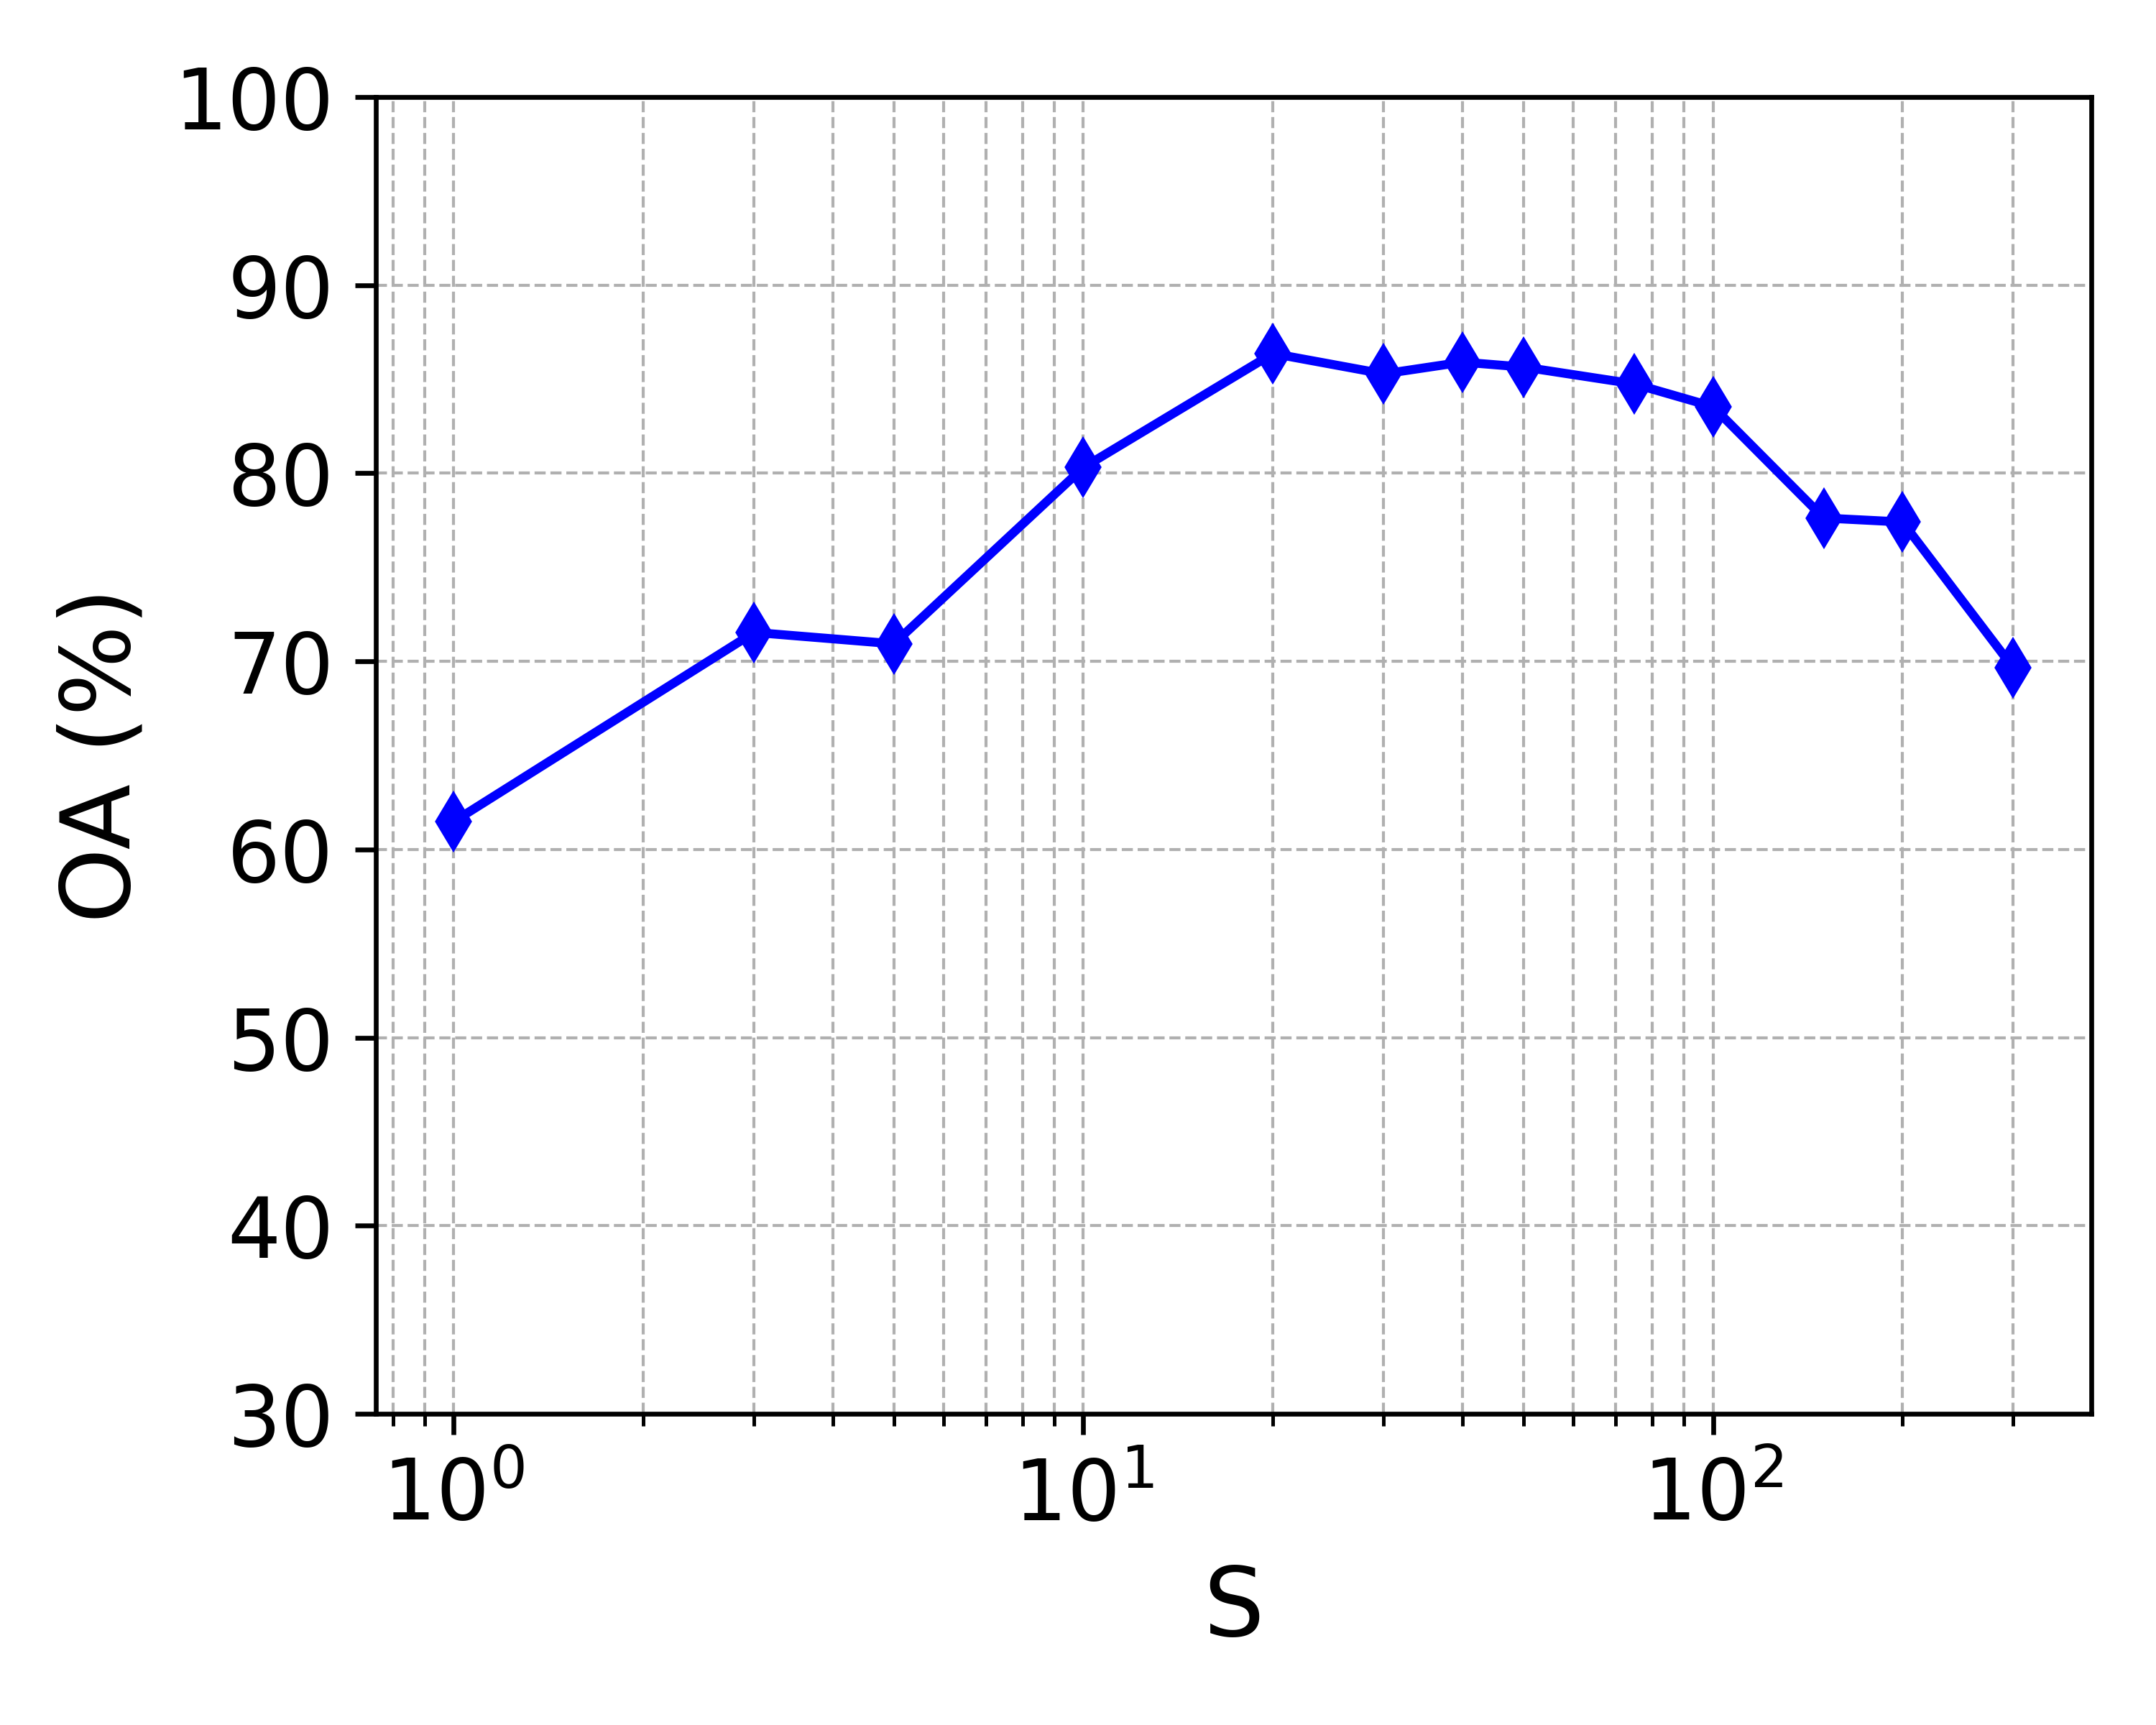
\includegraphics[width=\textwidth]{media/Exp1_T_20.png}
		\caption{}
	\end{subfigure}
	\begin{subfigure}[b]{0.4\textwidth}
		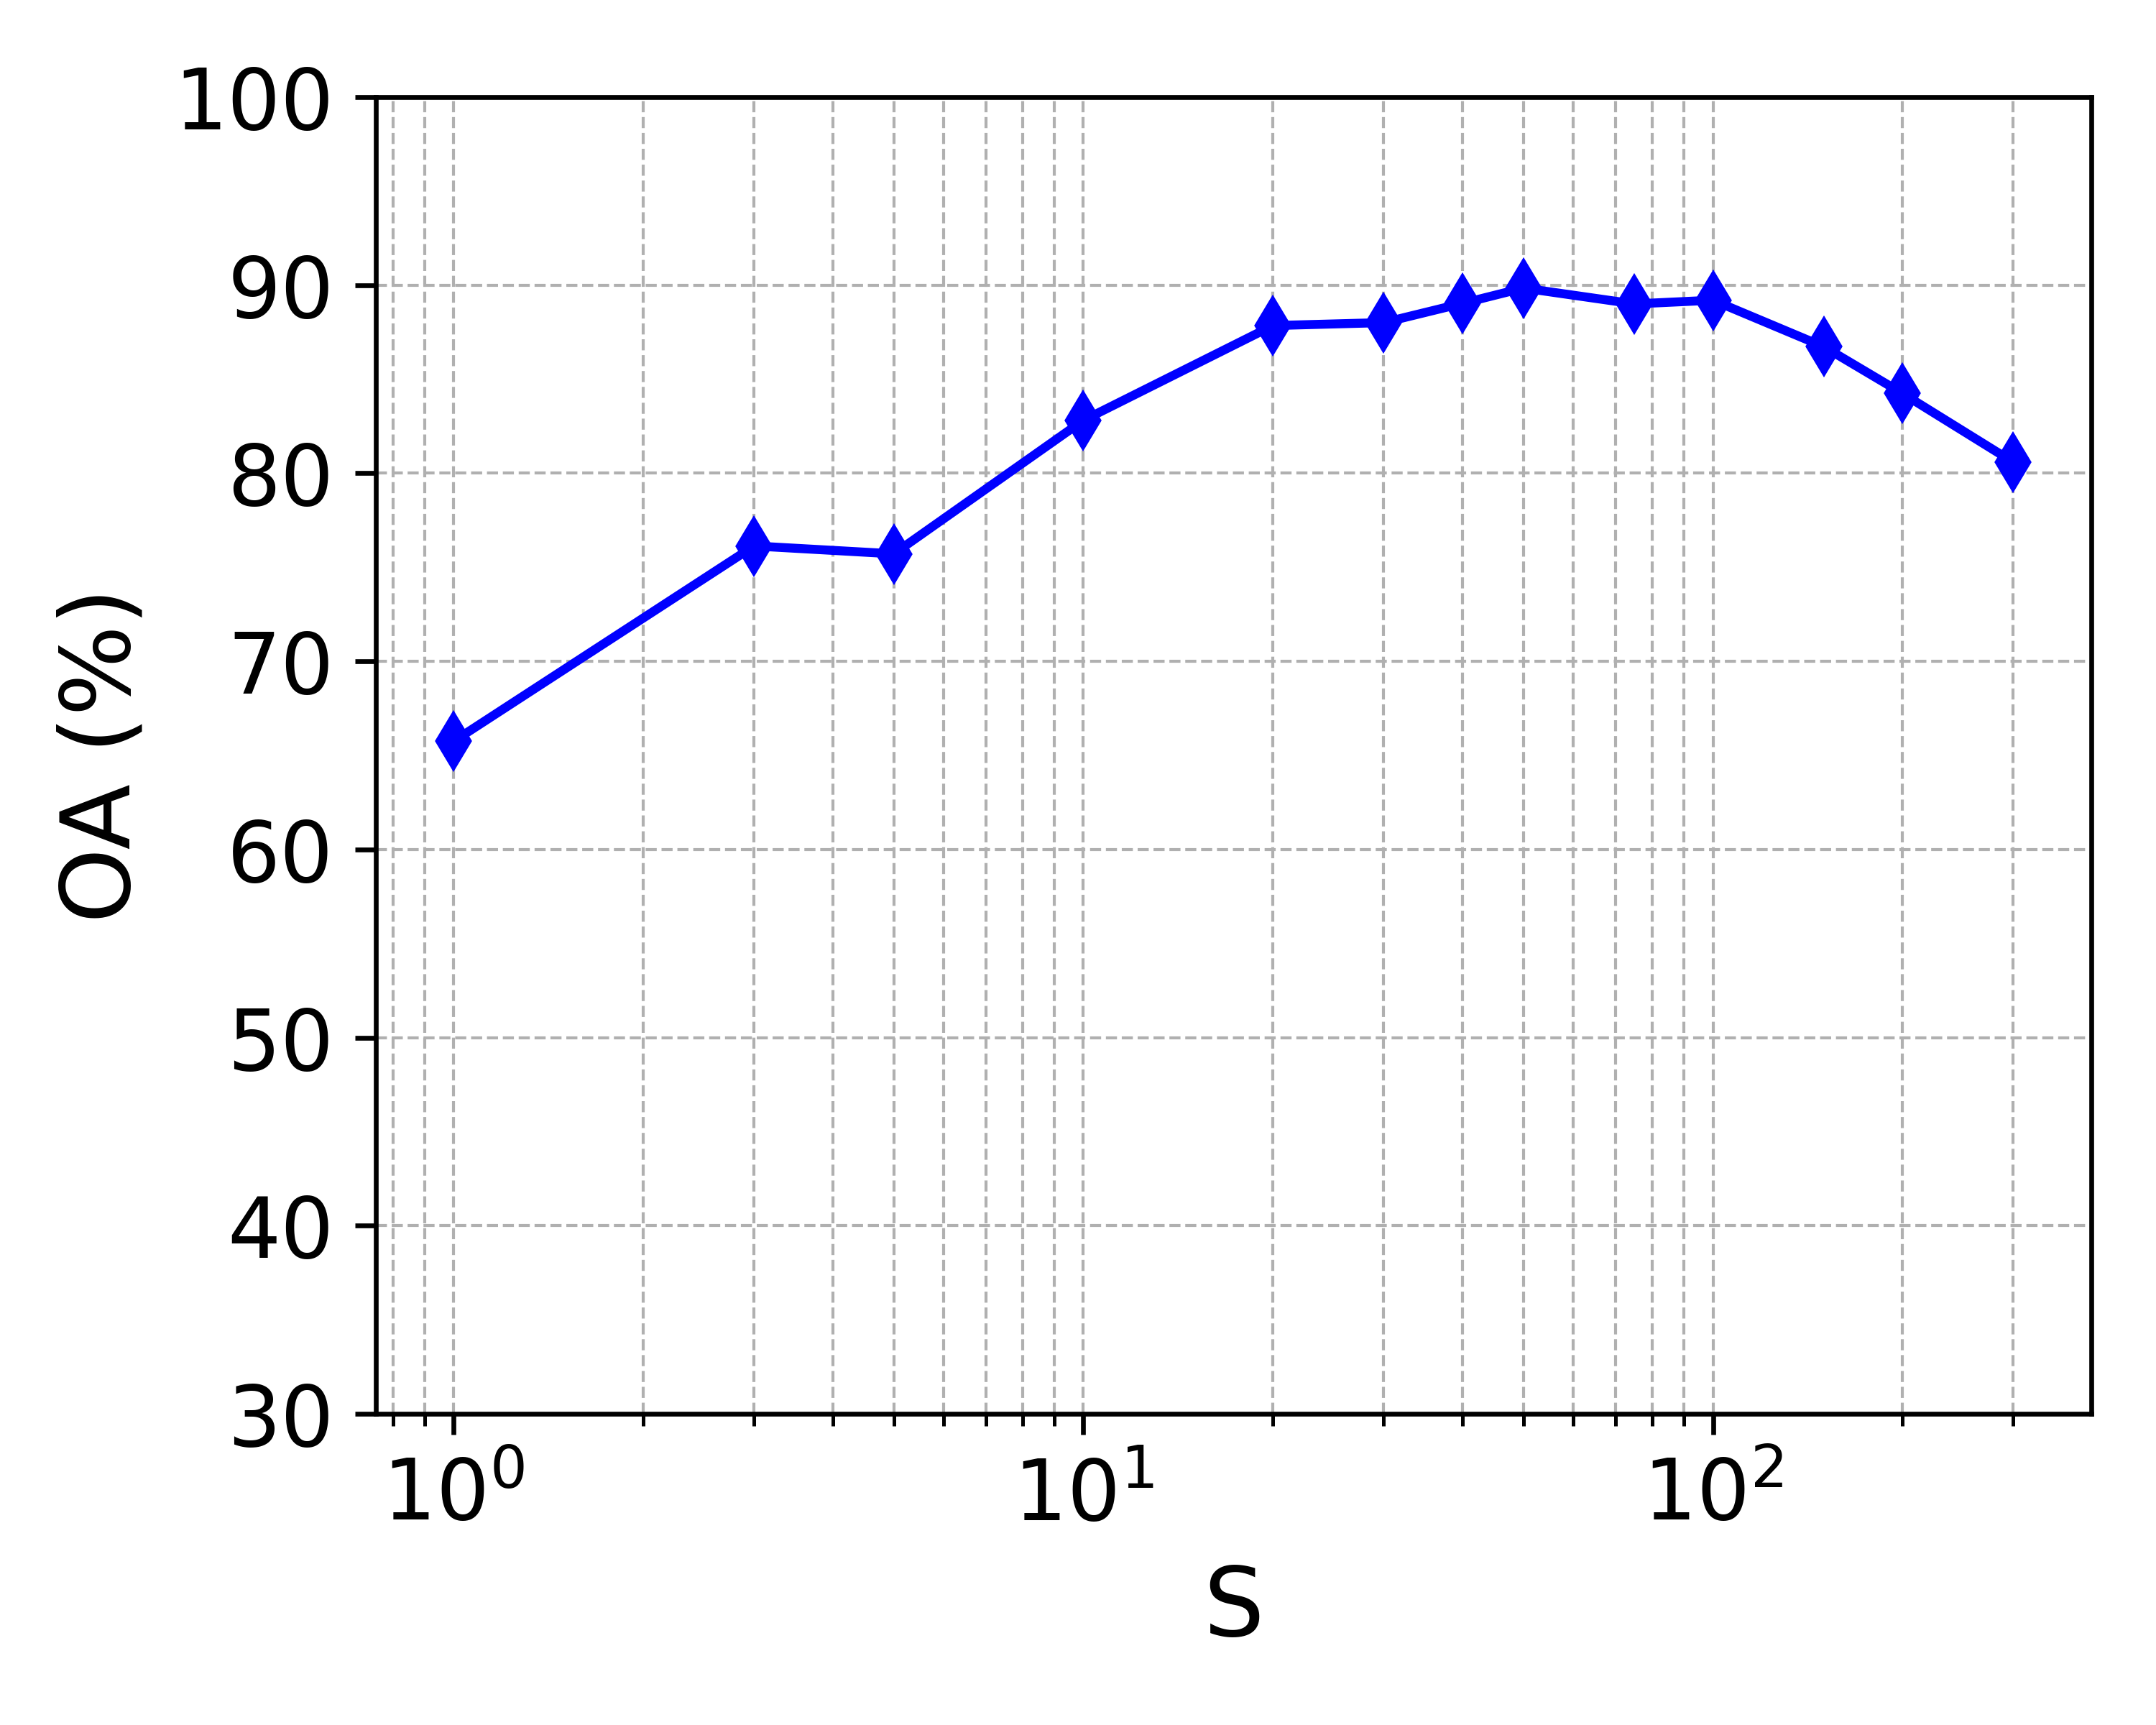
\includegraphics[width=\textwidth]{media/Exp1_T_30.png}
		\caption{}
	\end{subfigure}
	\caption{Influence of the number of superpixels on the overall classification accuracy of the SuperPCA method for the Indian Pines dataset when the training size is (a) 5, (b) 10, (c) 20 and (d) 30 samples per class.}
	\label{fig:exp1}
\end{figure}

Next, we examine the impact of the number of reconstruction neighbors on the performance of the S3-PCA method. Based on the previous experiment, the number of superpixels is fixed at $S = 50$. Dimensionality reduction is performed using S3-PCA with $k = \{5, 7, 9, 11, 13, 15, 17, 19\}$, followed by classification using $T = 30$ training samples per class. The results are shown in Figure~\ref{fig:exp2a}.

The overall accuracy first increases with $k$, but then declines beyond a certain point. A small $k$ results in insufficient spatial information for reliable reconstruction, while a large $k$ risks including neighbors from different classes, degrading the quality of reconstruction. This highlights the importance of carefully selecting $k$ to balance locality and class consistency. From this experiment, the optimal value of $k$ for the Indian Pines dataset is found to be $k = 13$.

\begin{figure}[h!]
	\centering
	\begin{subfigure}[b]{0.4\textwidth}
		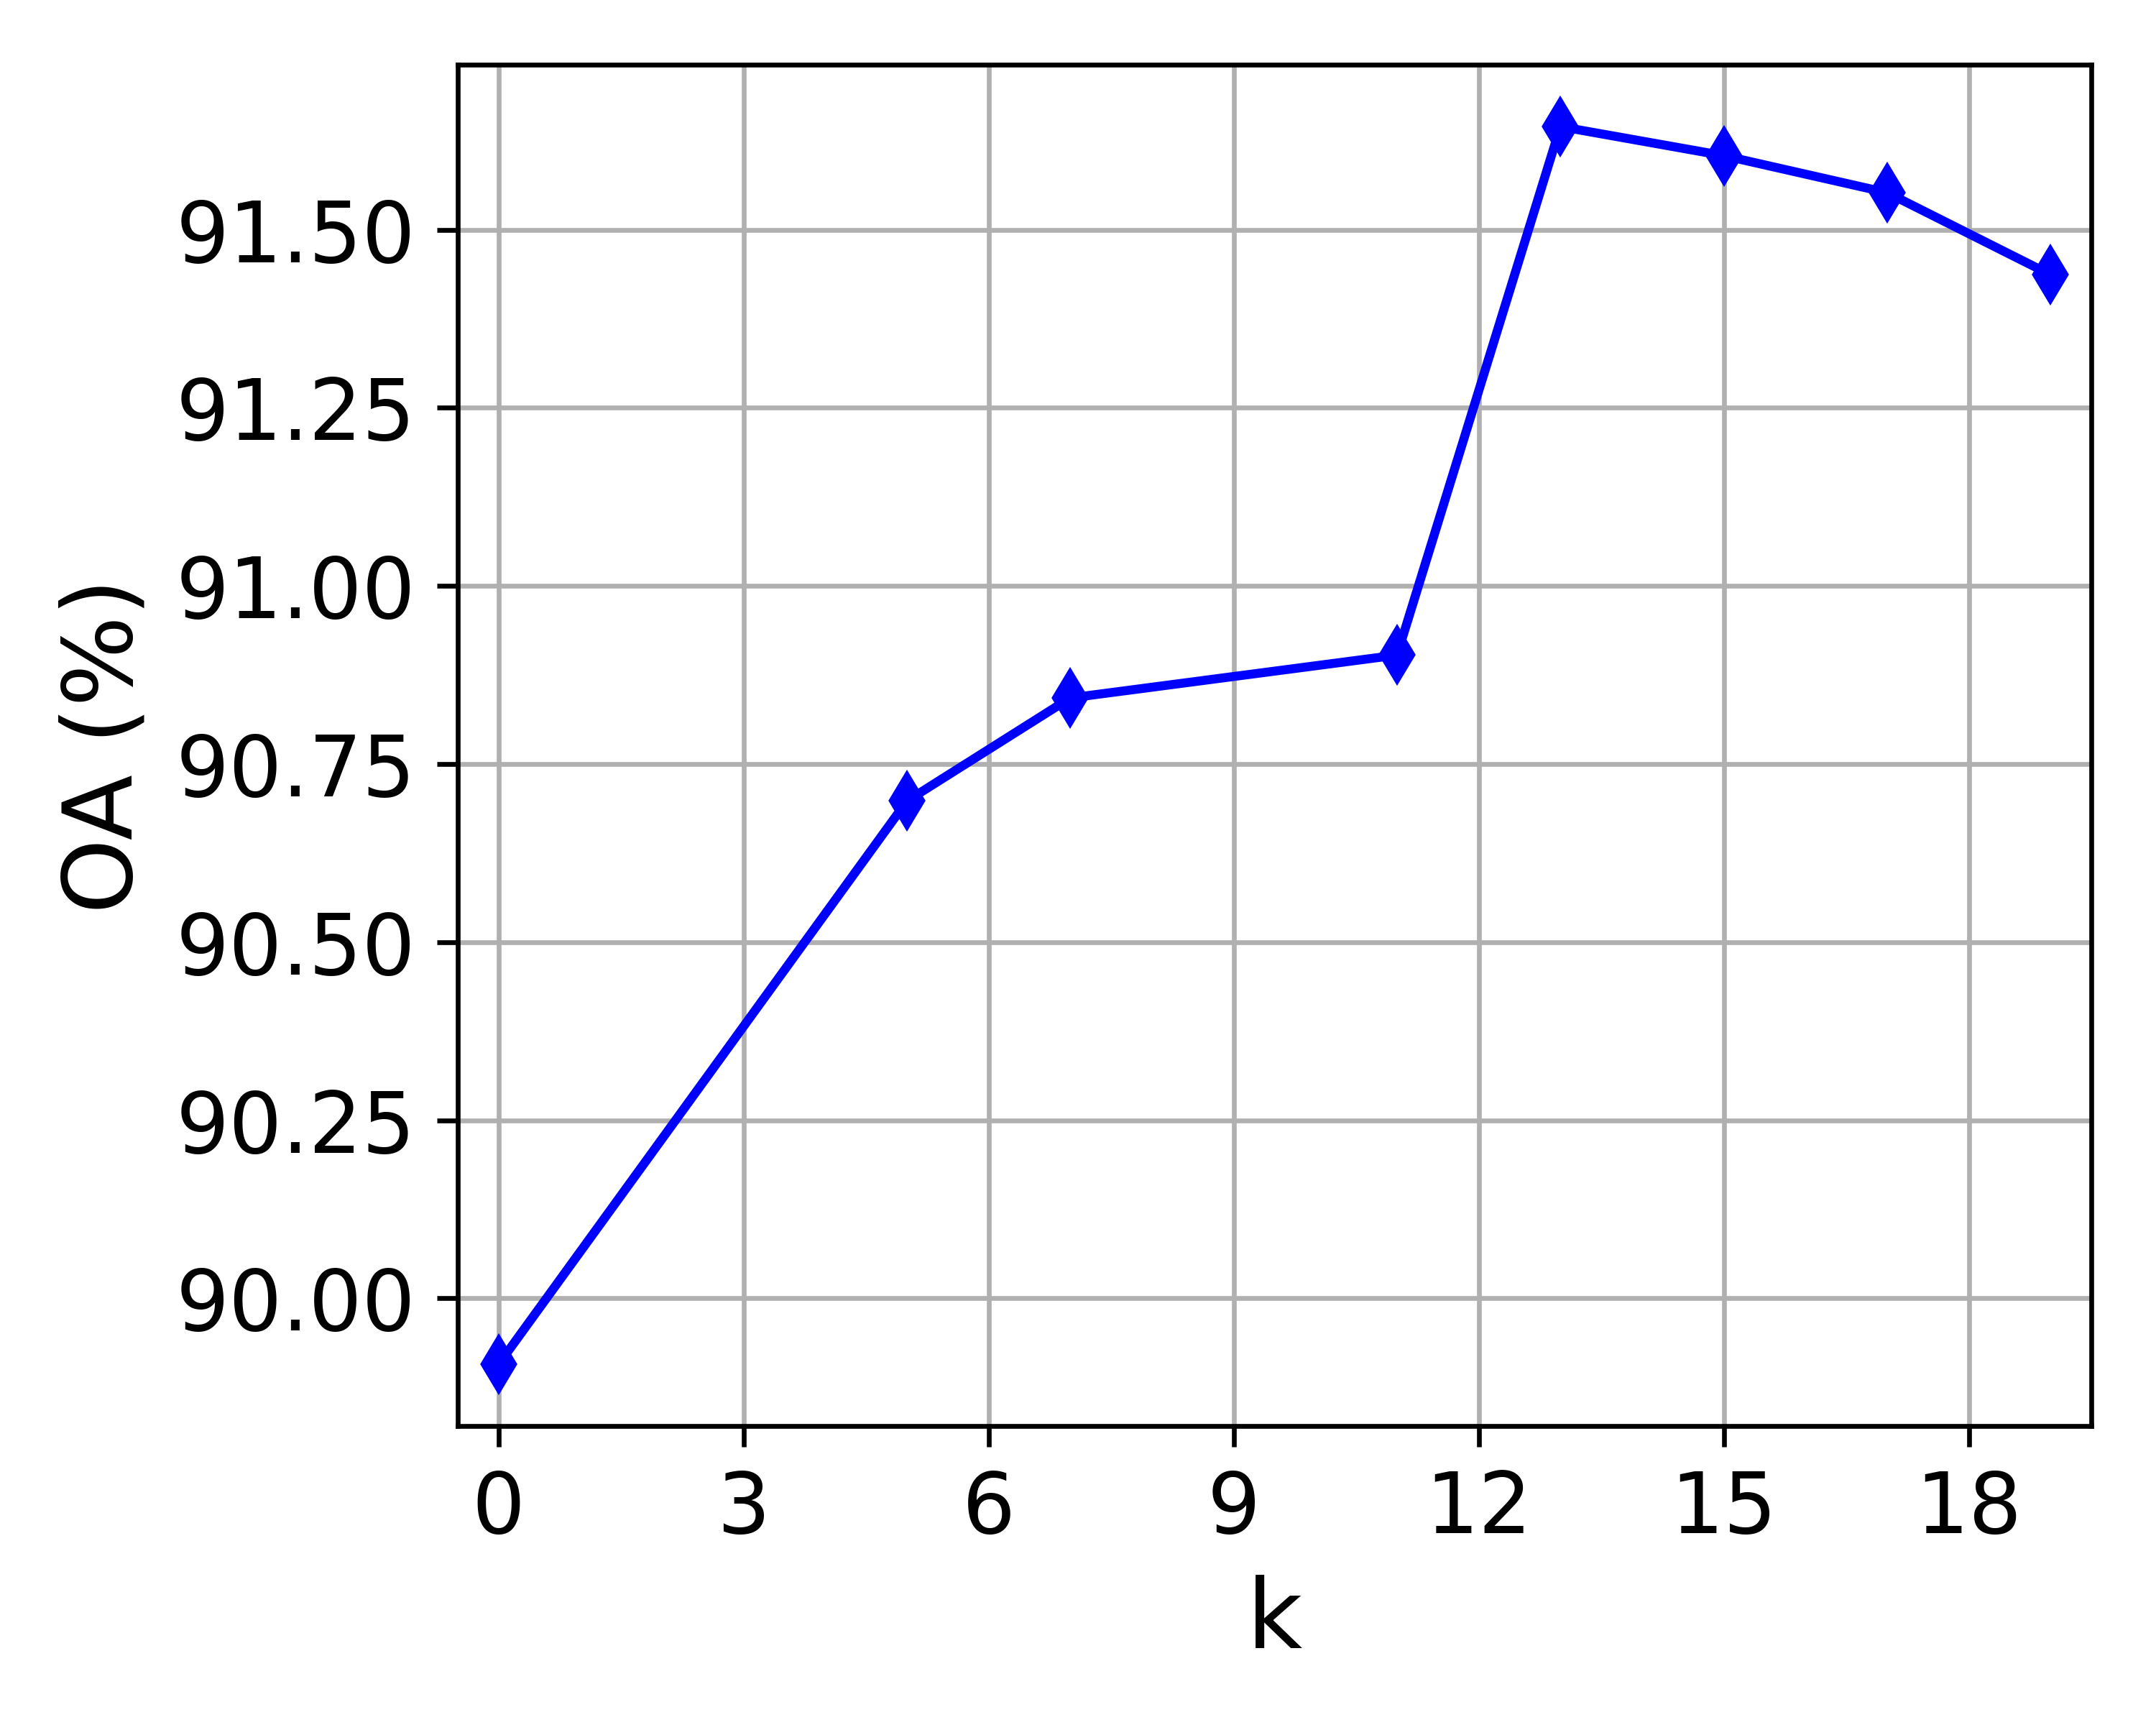
\includegraphics[width=\textwidth]{media/Exp2a.png}
		\caption{}
		\label{fig:exp2a}
	\end{subfigure}
	\begin{subfigure}[b]{0.4\textwidth}
		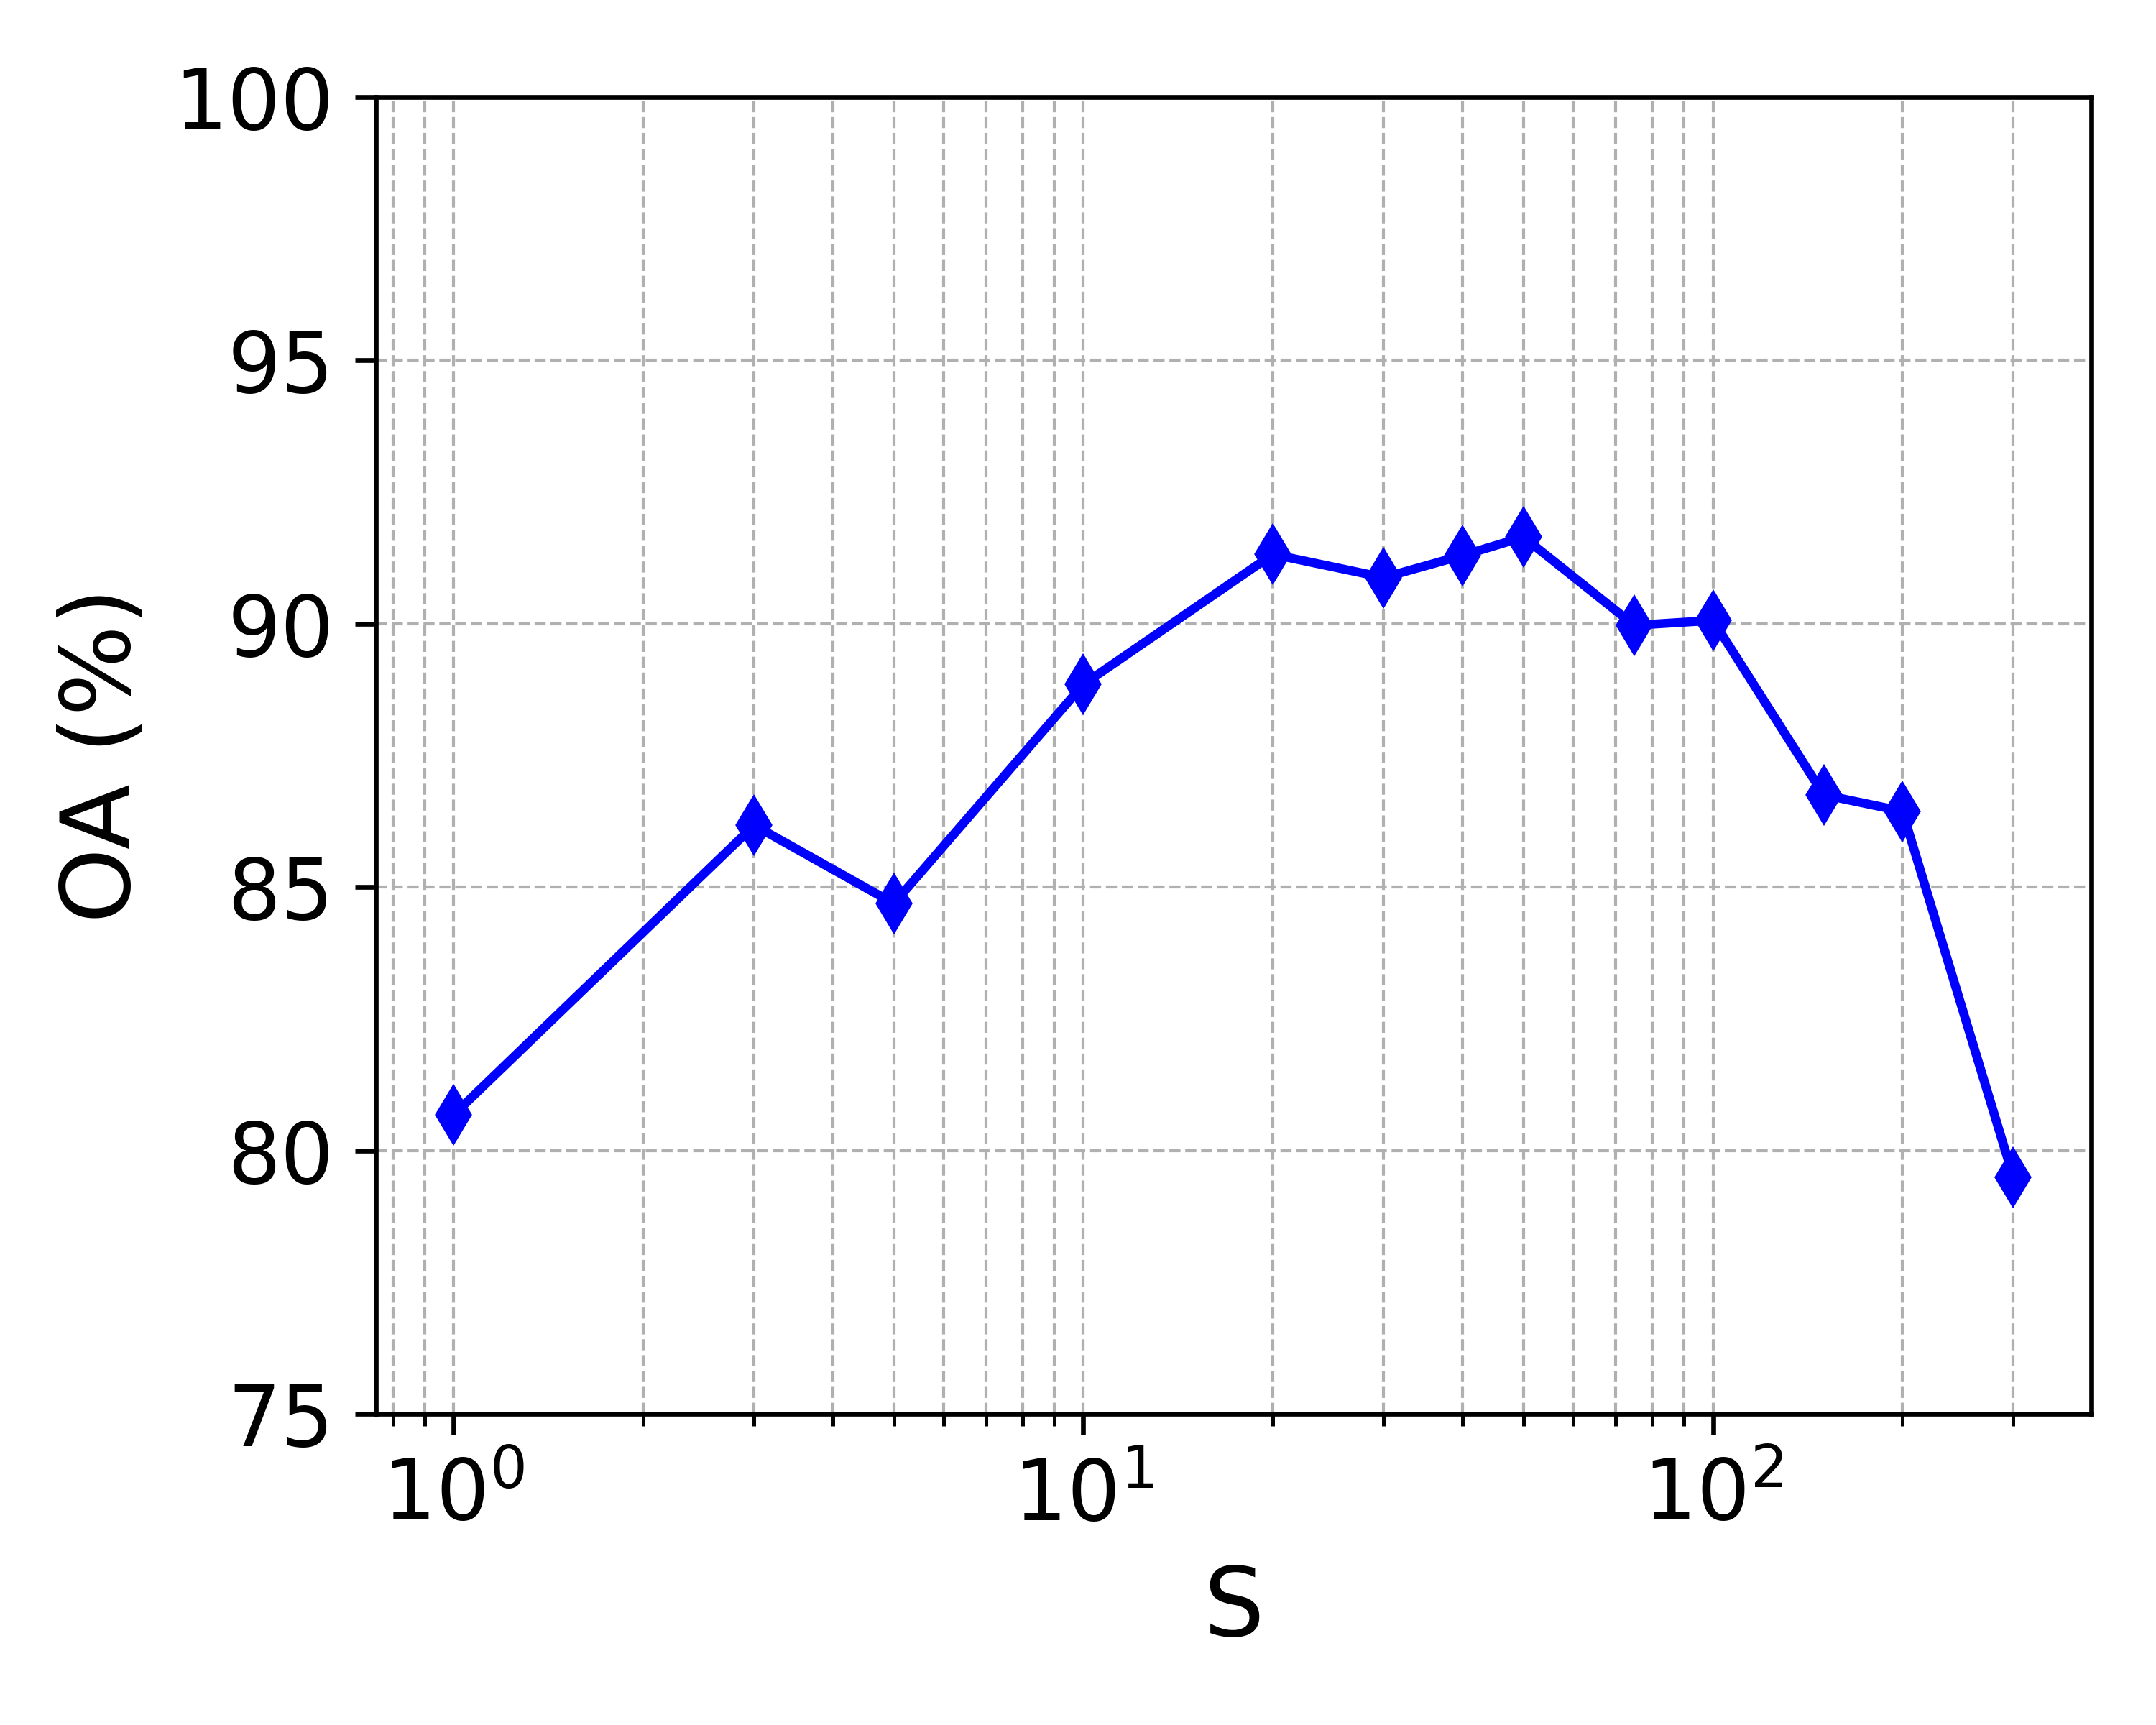
\includegraphics[width=\textwidth]{media/Exp2b.png}
		\caption{}
		\label{fig:exp2b}
	\end{subfigure}
	
	\caption{Overall accuracy of the S3-PCA method for the Indian Pines dataset (a) for different numbers of reconstruction neighbors $k$ when the number of superpixels $S$ is set to 50, and (b) for different numbers of superpixels $S$ when the number of reconstruction neighbors is optimally set to 13.}
	\label{fig:exp2}
\end{figure}

Finally, we fix the number of reconstruction neighbors at $k = 13$ and evaluate the S3-PCA method across varying numbers of superpixels $S = \{1, 3, 5, 10, 20, 30, 40, 50, 75, 100, 150, 200, 300\}$. Classification is performed using $T = 30$ training samples per class. As shown in Figure~\ref{fig:exp2b}, we observe a similar trend in the variation of overall accuracy with respect to $S$ as seen with SuperPCA. Performance improves initially, peaks, and then declines with very high or very low values of $S$. The optimal number of superpixels remains $S = 50$ for the Indian Pines dataset.

\subsection{Performance Evaluation}

To evaluate the effectiveness of the SuperPCA and S3-PCA methods, we compare their classification performance with that of conventional PCA and raw hyperspectral data. Dimensionality reduction is performed using four approaches: Raw (no dimensionality reduction), PCA, SuperPCA, and S3-PCA. Optimal parameters from the previous experiments are used for SuperPCA and S3-PCA. Classification is then carried out using an SVM classifier with \( T = \{5, 10, 20, 30, 40, 50, 60\} \) training samples per class.

Figure~\ref{fig:exp3} presents the overall accuracy obtained by each method across the different training sizes. It is evident that PCA consistently underperforms, even compared to using the raw data directly. This suggests that PCA fails to capture informative low-dimensional features in this context. In contrast, SuperPCA significantly improves performance over both raw and PCA-based approaches for all values of \( T \). S3-PCA provides a further improvement over SuperPCA, highlighting the benefits of incorporating spatial reconstruction in the dimensionality reduction process.

Figure~\ref{fig:exp3_maps} shows the classification maps obtained using the different methods. Notably, S3-PCA exhibits improved accuracy in regions with mixed ground truth labels, i.e., where neighboring classes are closely situated spatially.

\begin{figure}[h!]
	\centering
	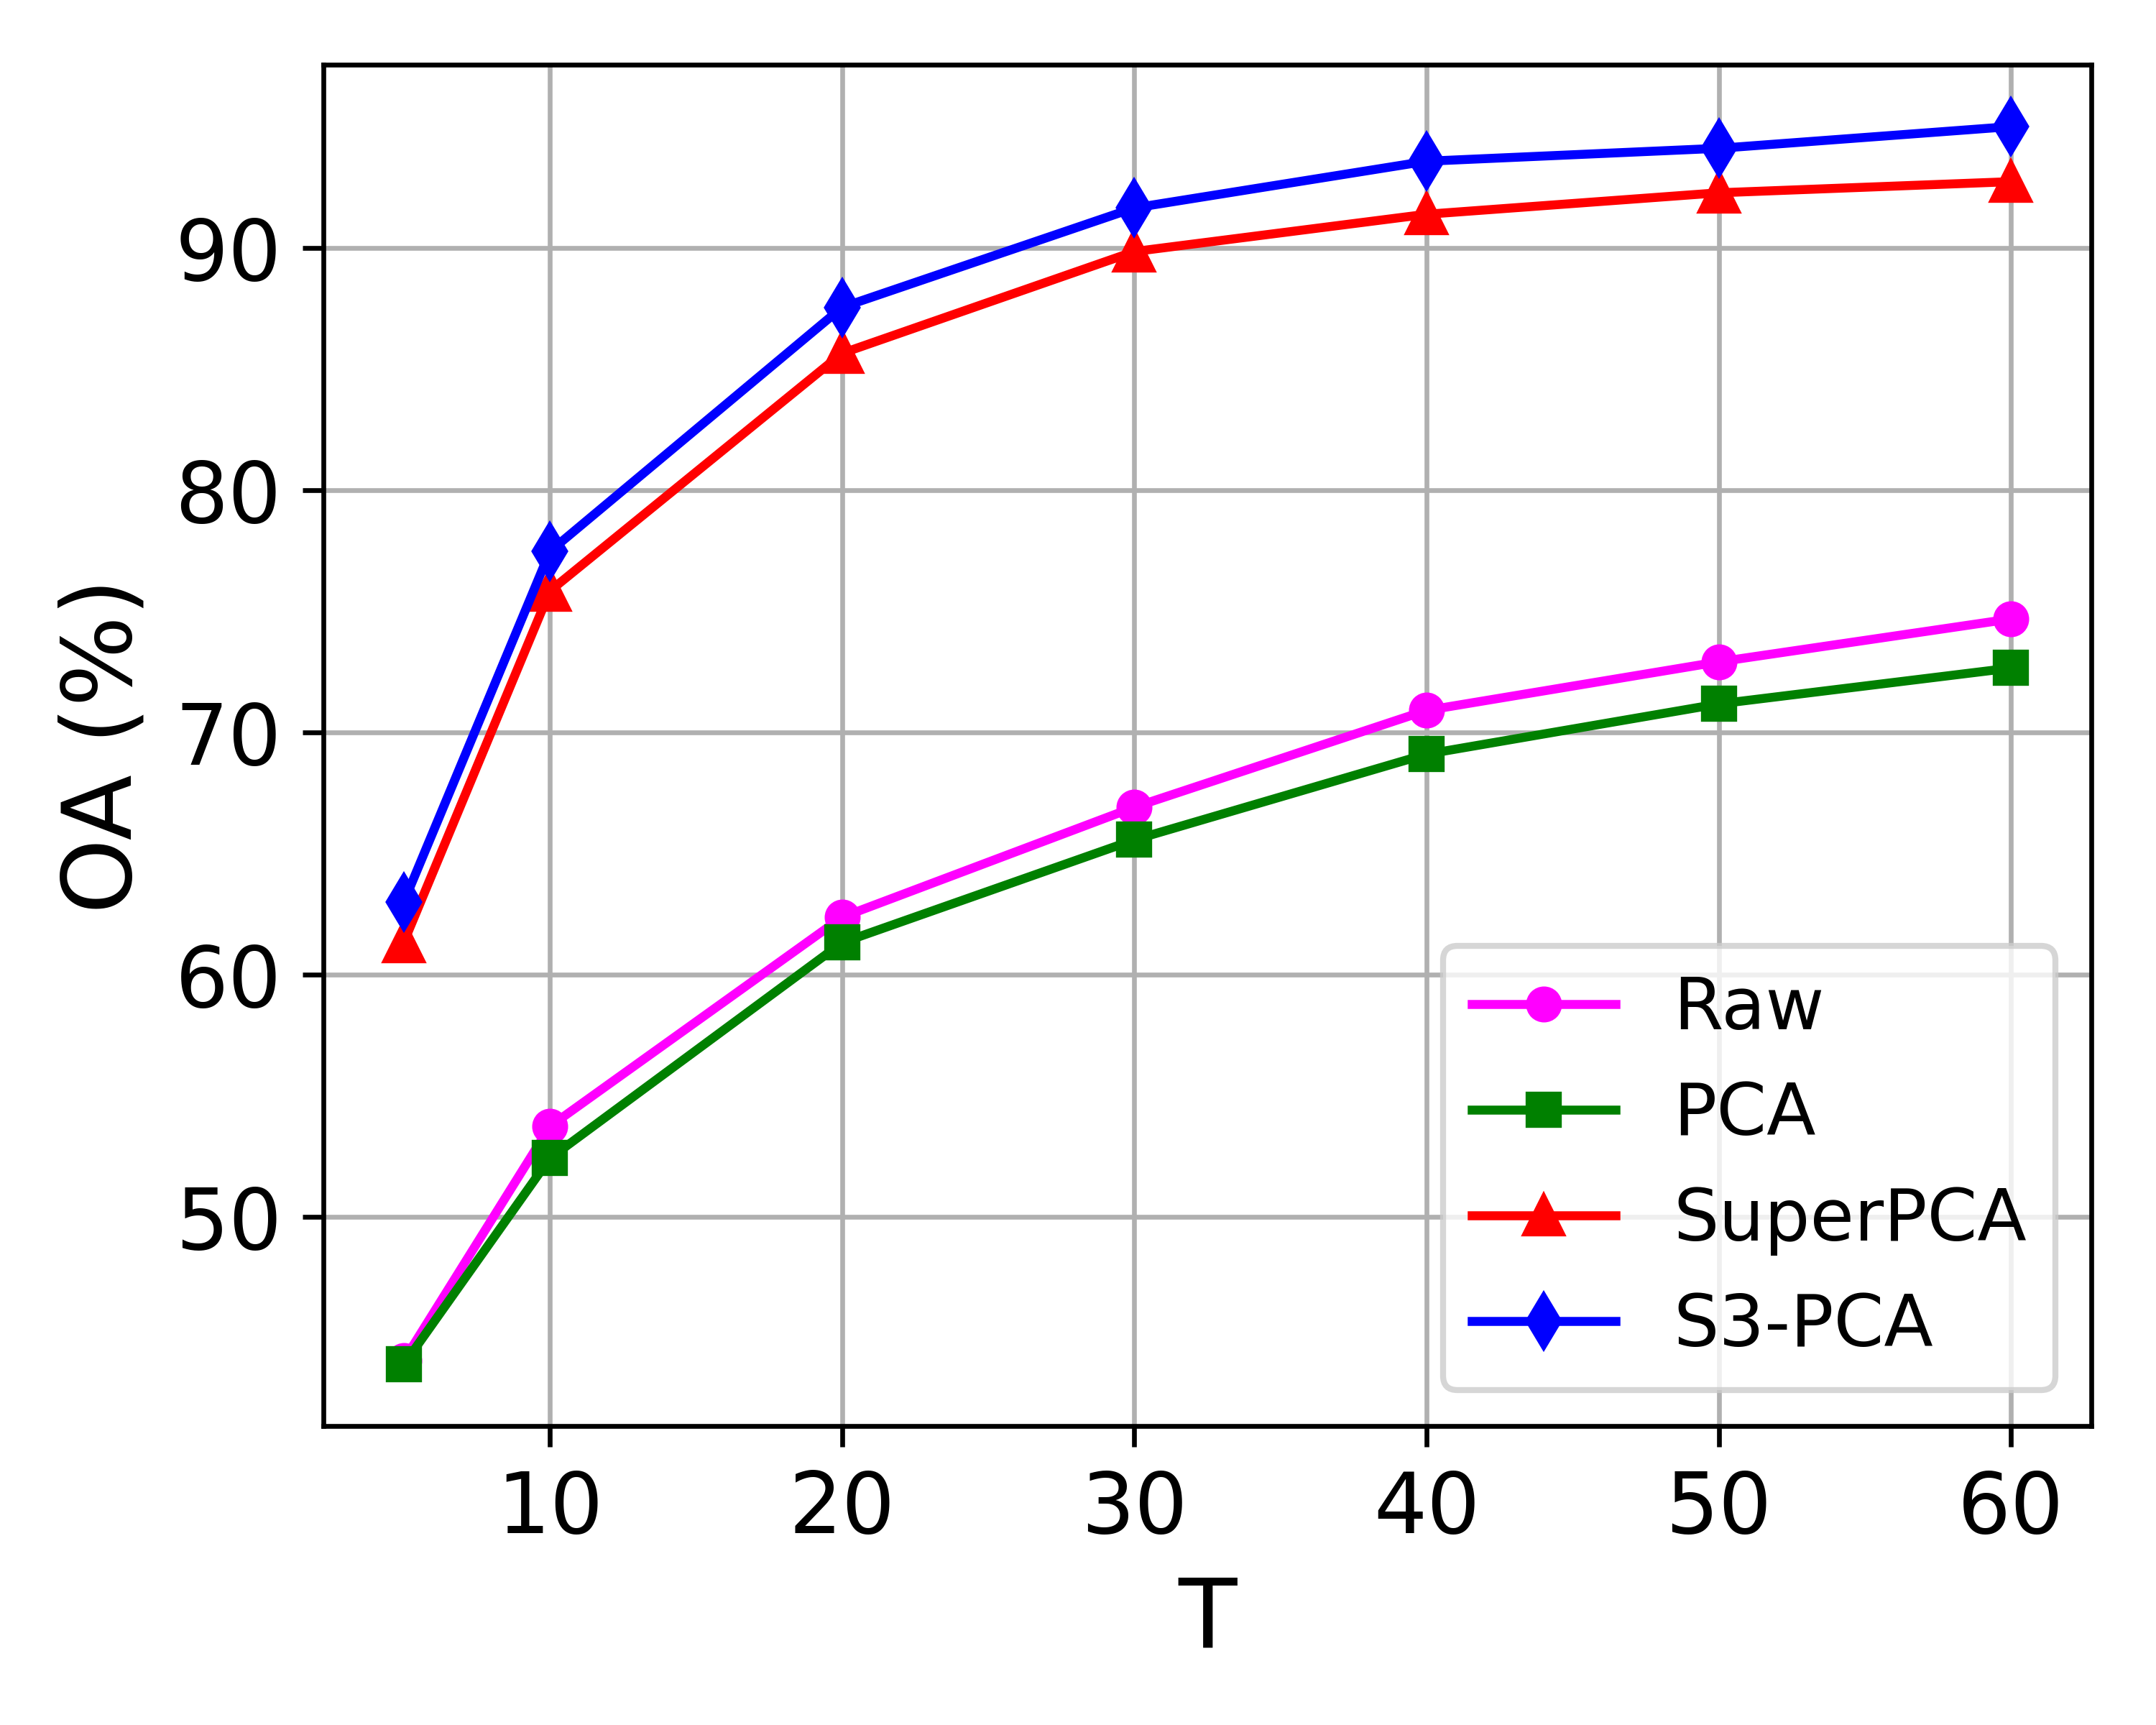
\includegraphics[width=0.4\textwidth]{media/Exp3.png}
	\caption{Overall classification accuracy on the Indian Pines dataset using various dimensionality reduction methods across different numbers of training samples per class.}
	\label{fig:exp3}
\end{figure}

\begin{figure}[h!]
	\centering
	\begin{subfigure}[b]{0.24\textwidth}
		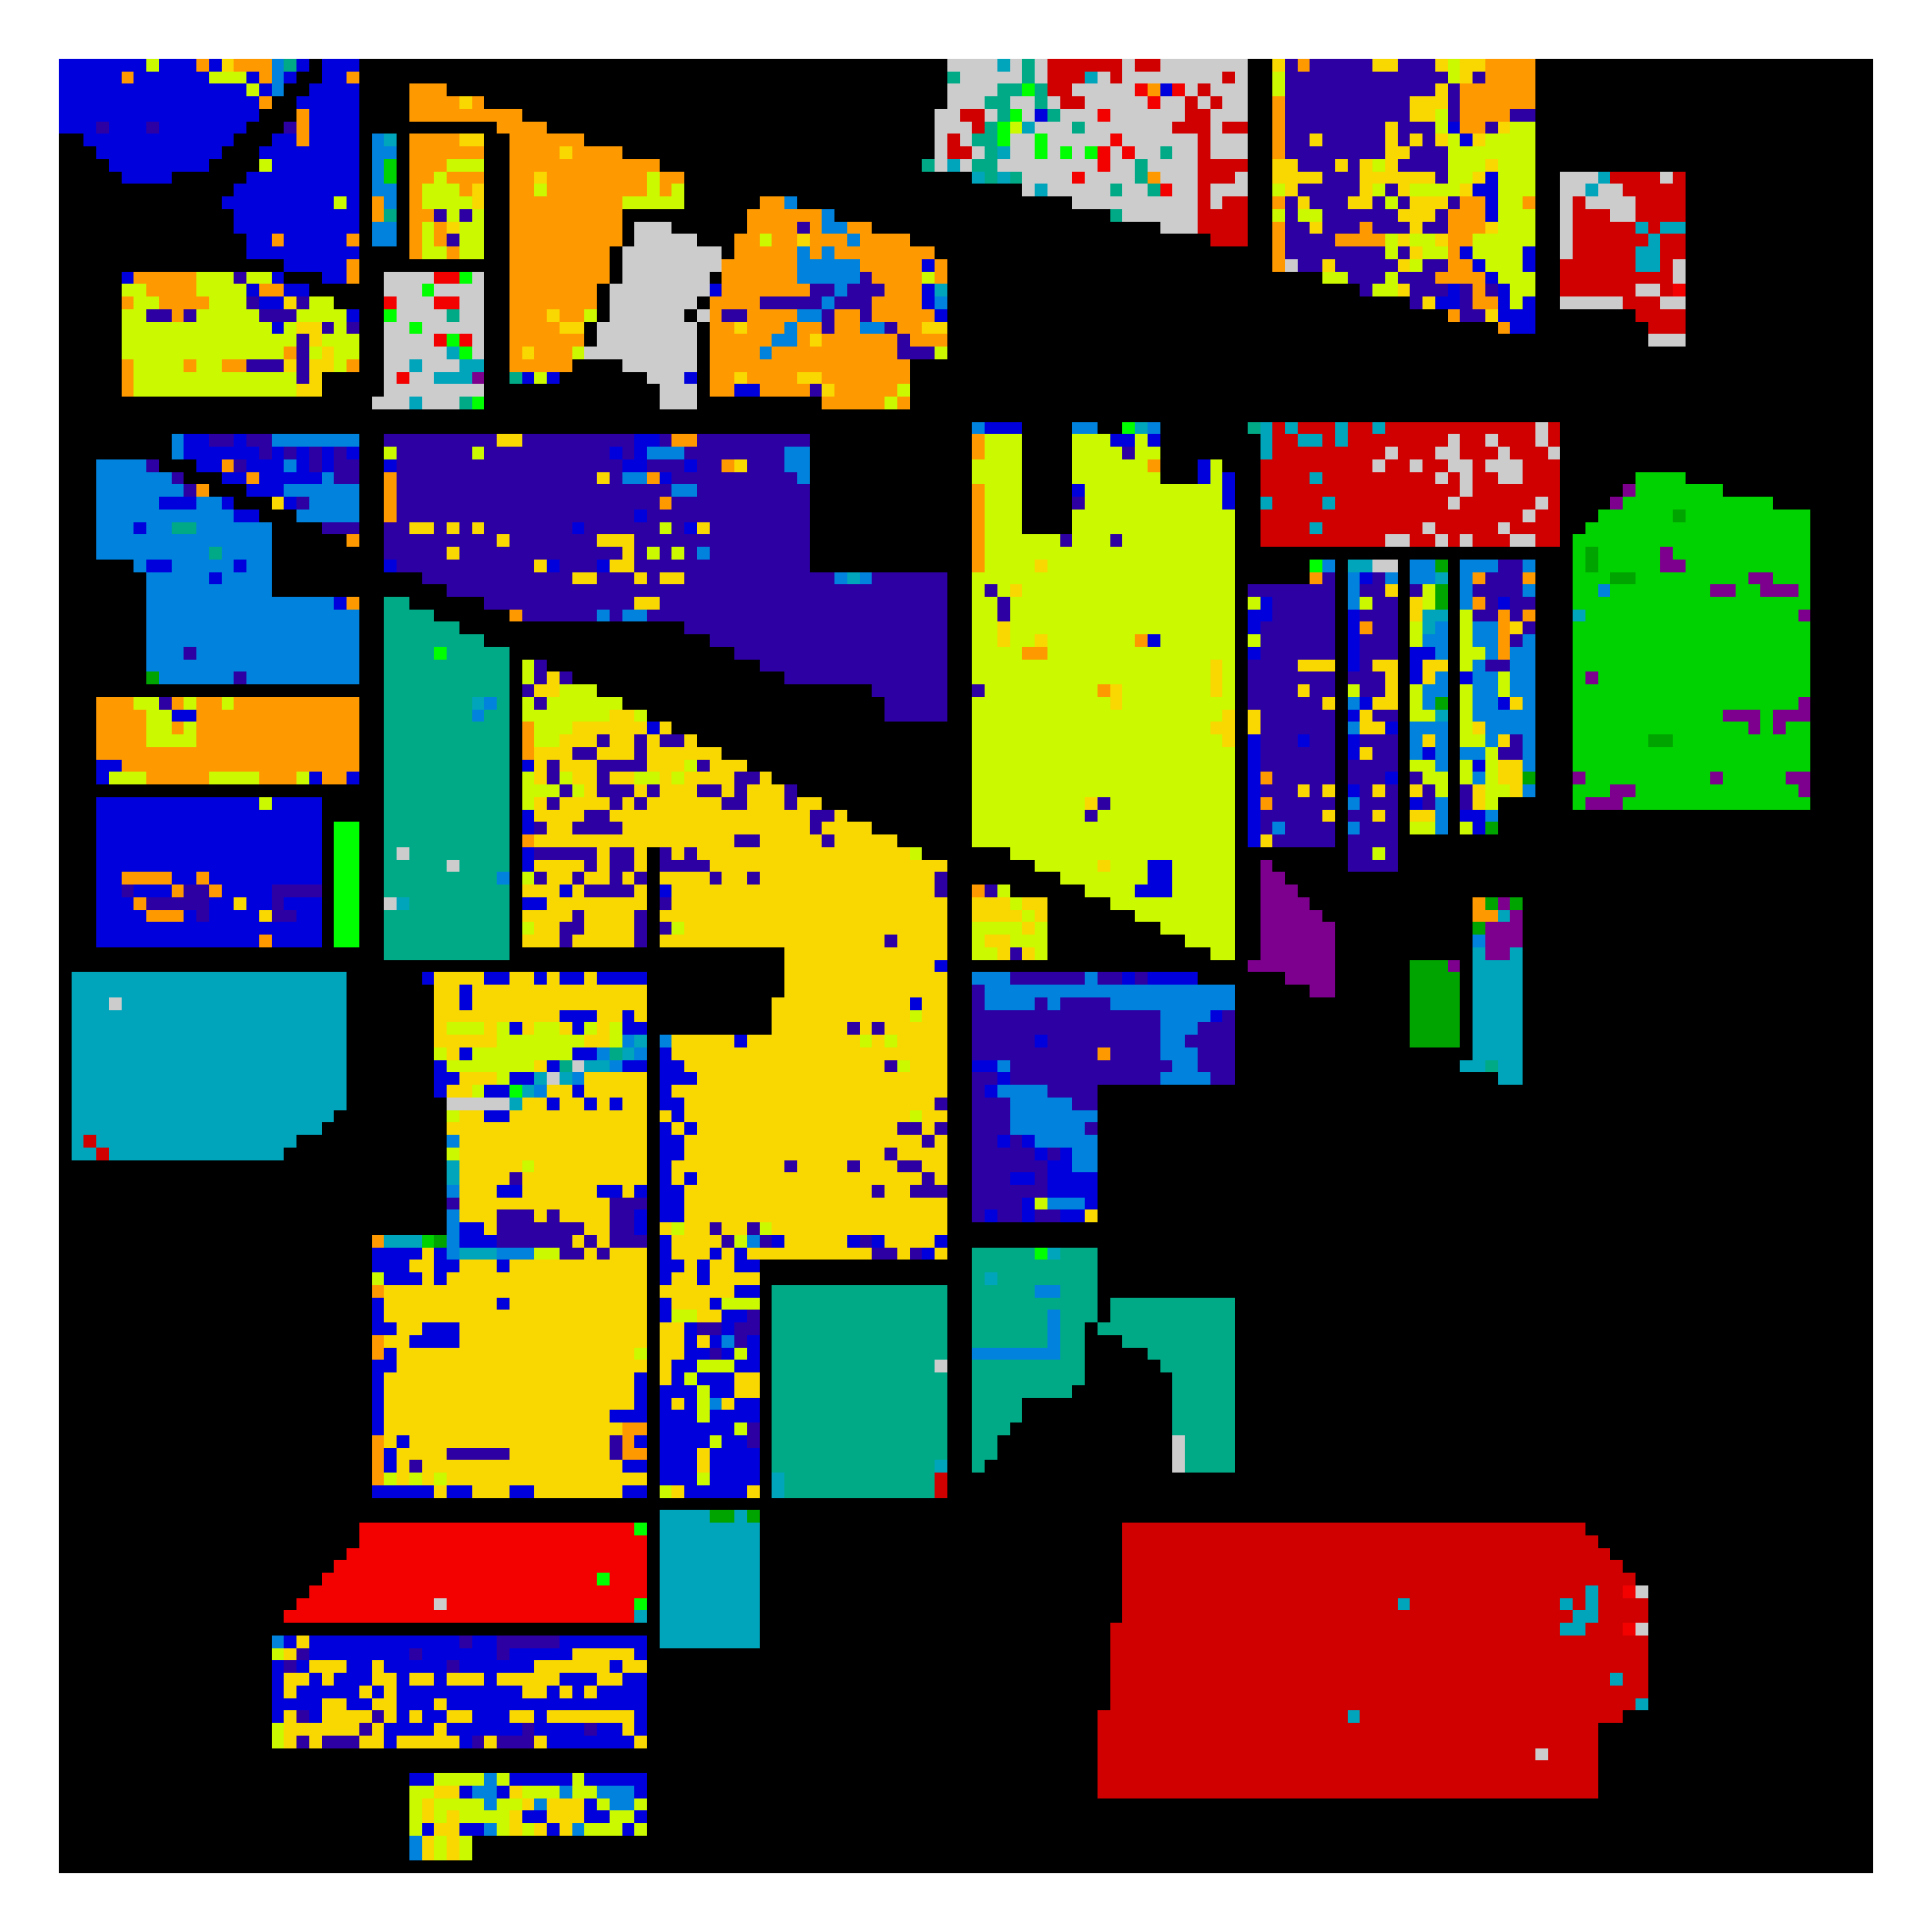
\includegraphics[width=\textwidth]{media/exp3_raw_class_map.png}
		\caption{OA = 66.92\%}
	\end{subfigure}
	\begin{subfigure}[b]{0.24\textwidth}
		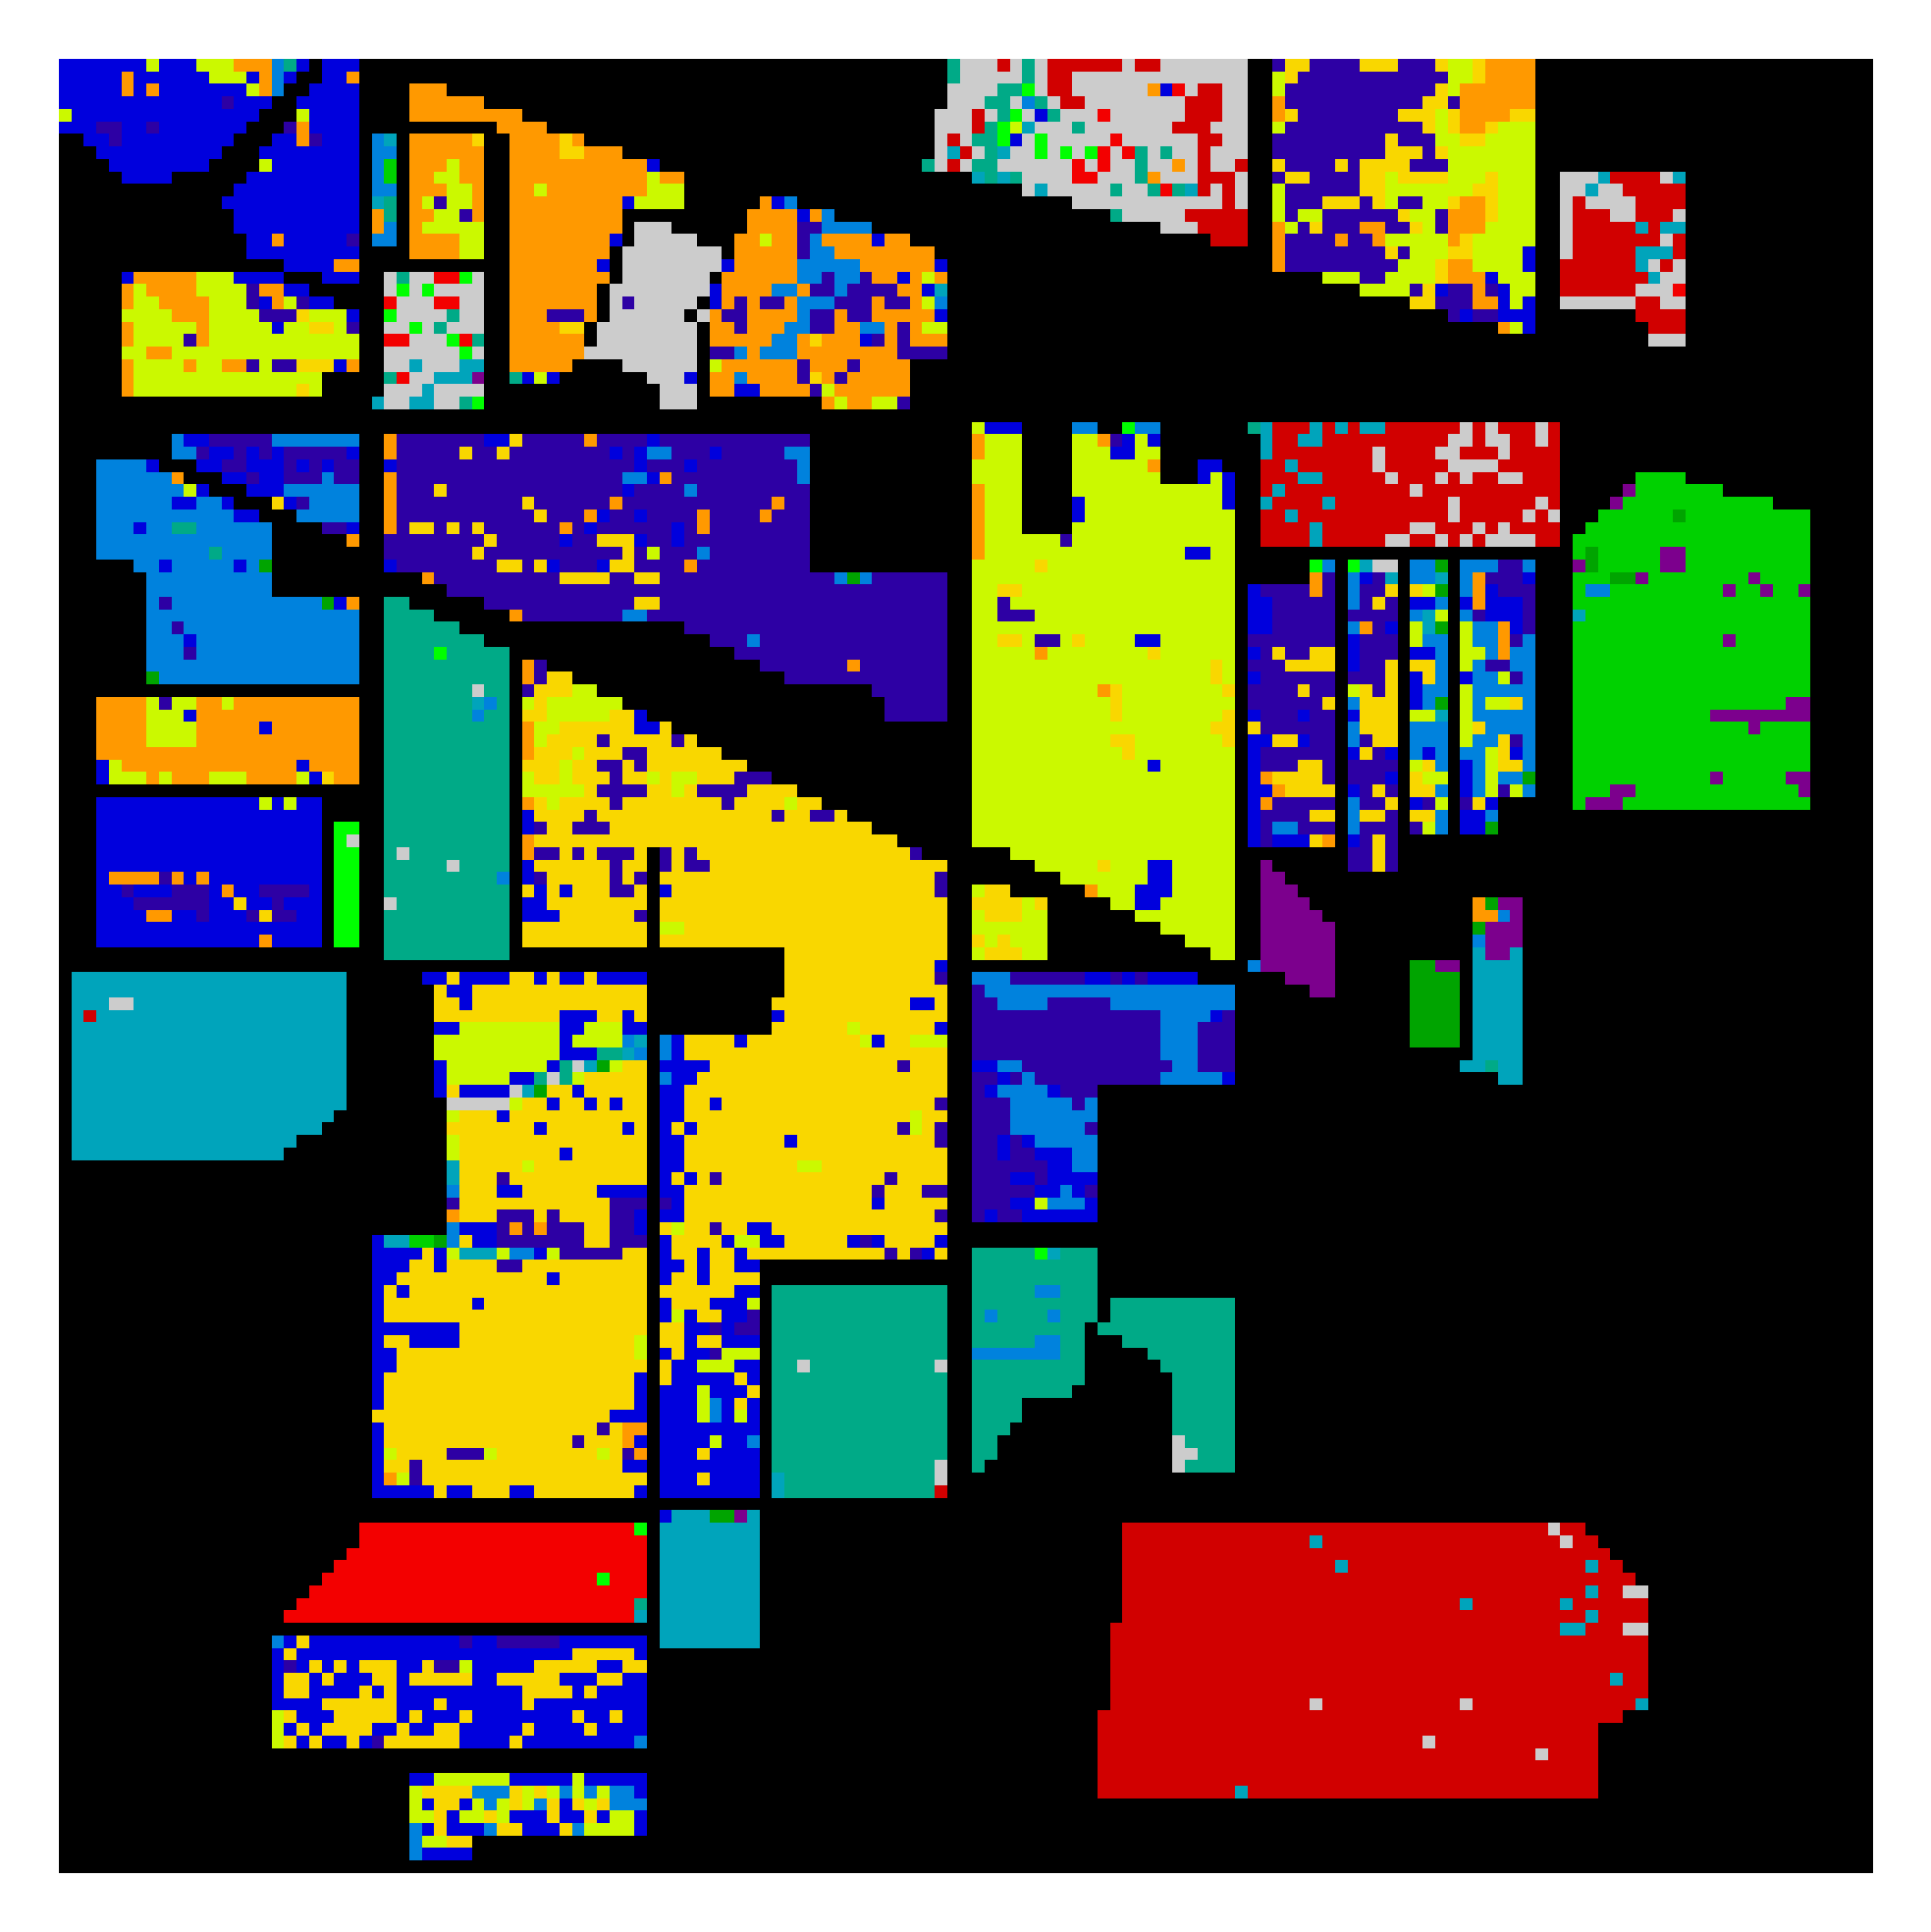
\includegraphics[width=\textwidth]{media/exp3_pca_class_map.png}
		\caption{OA = 65.57\%}
	\end{subfigure}
	\begin{subfigure}[b]{0.24\textwidth}
		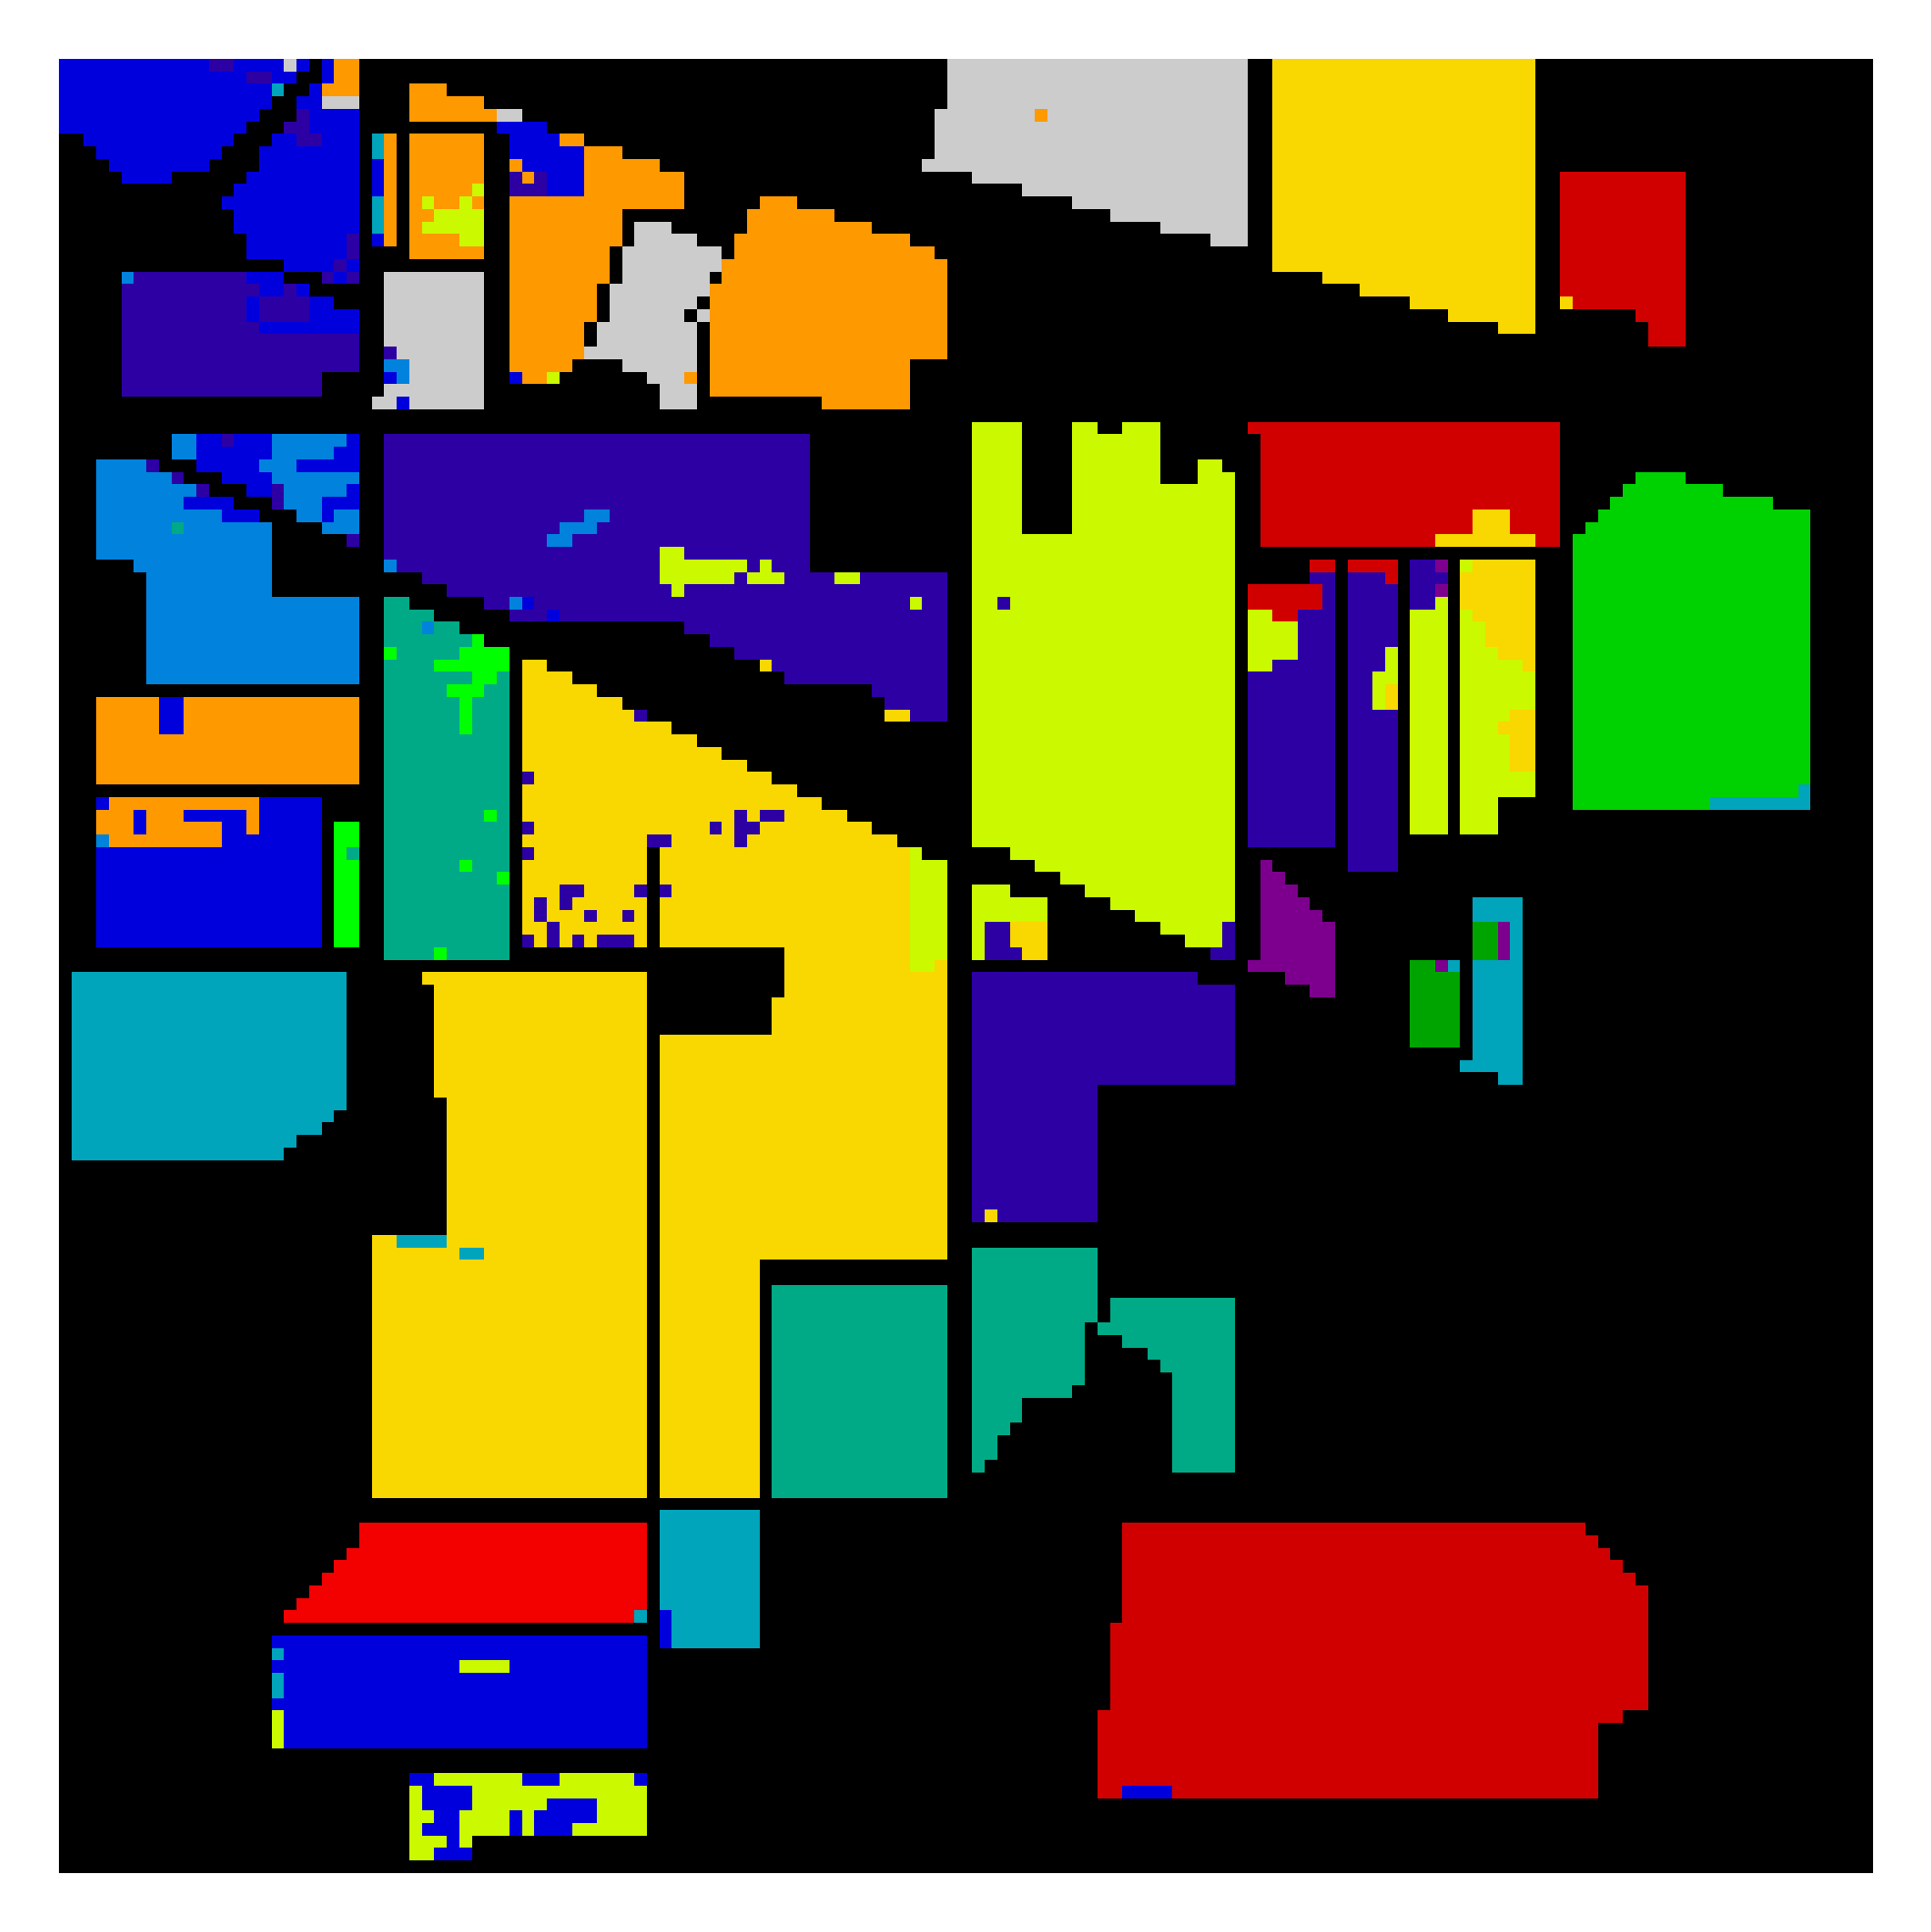
\includegraphics[width=\textwidth]{media/exp3_superpca_class_map.png}
		\caption{OA = 89.84\%}
	\end{subfigure}
	\begin{subfigure}[b]{0.24\textwidth}
		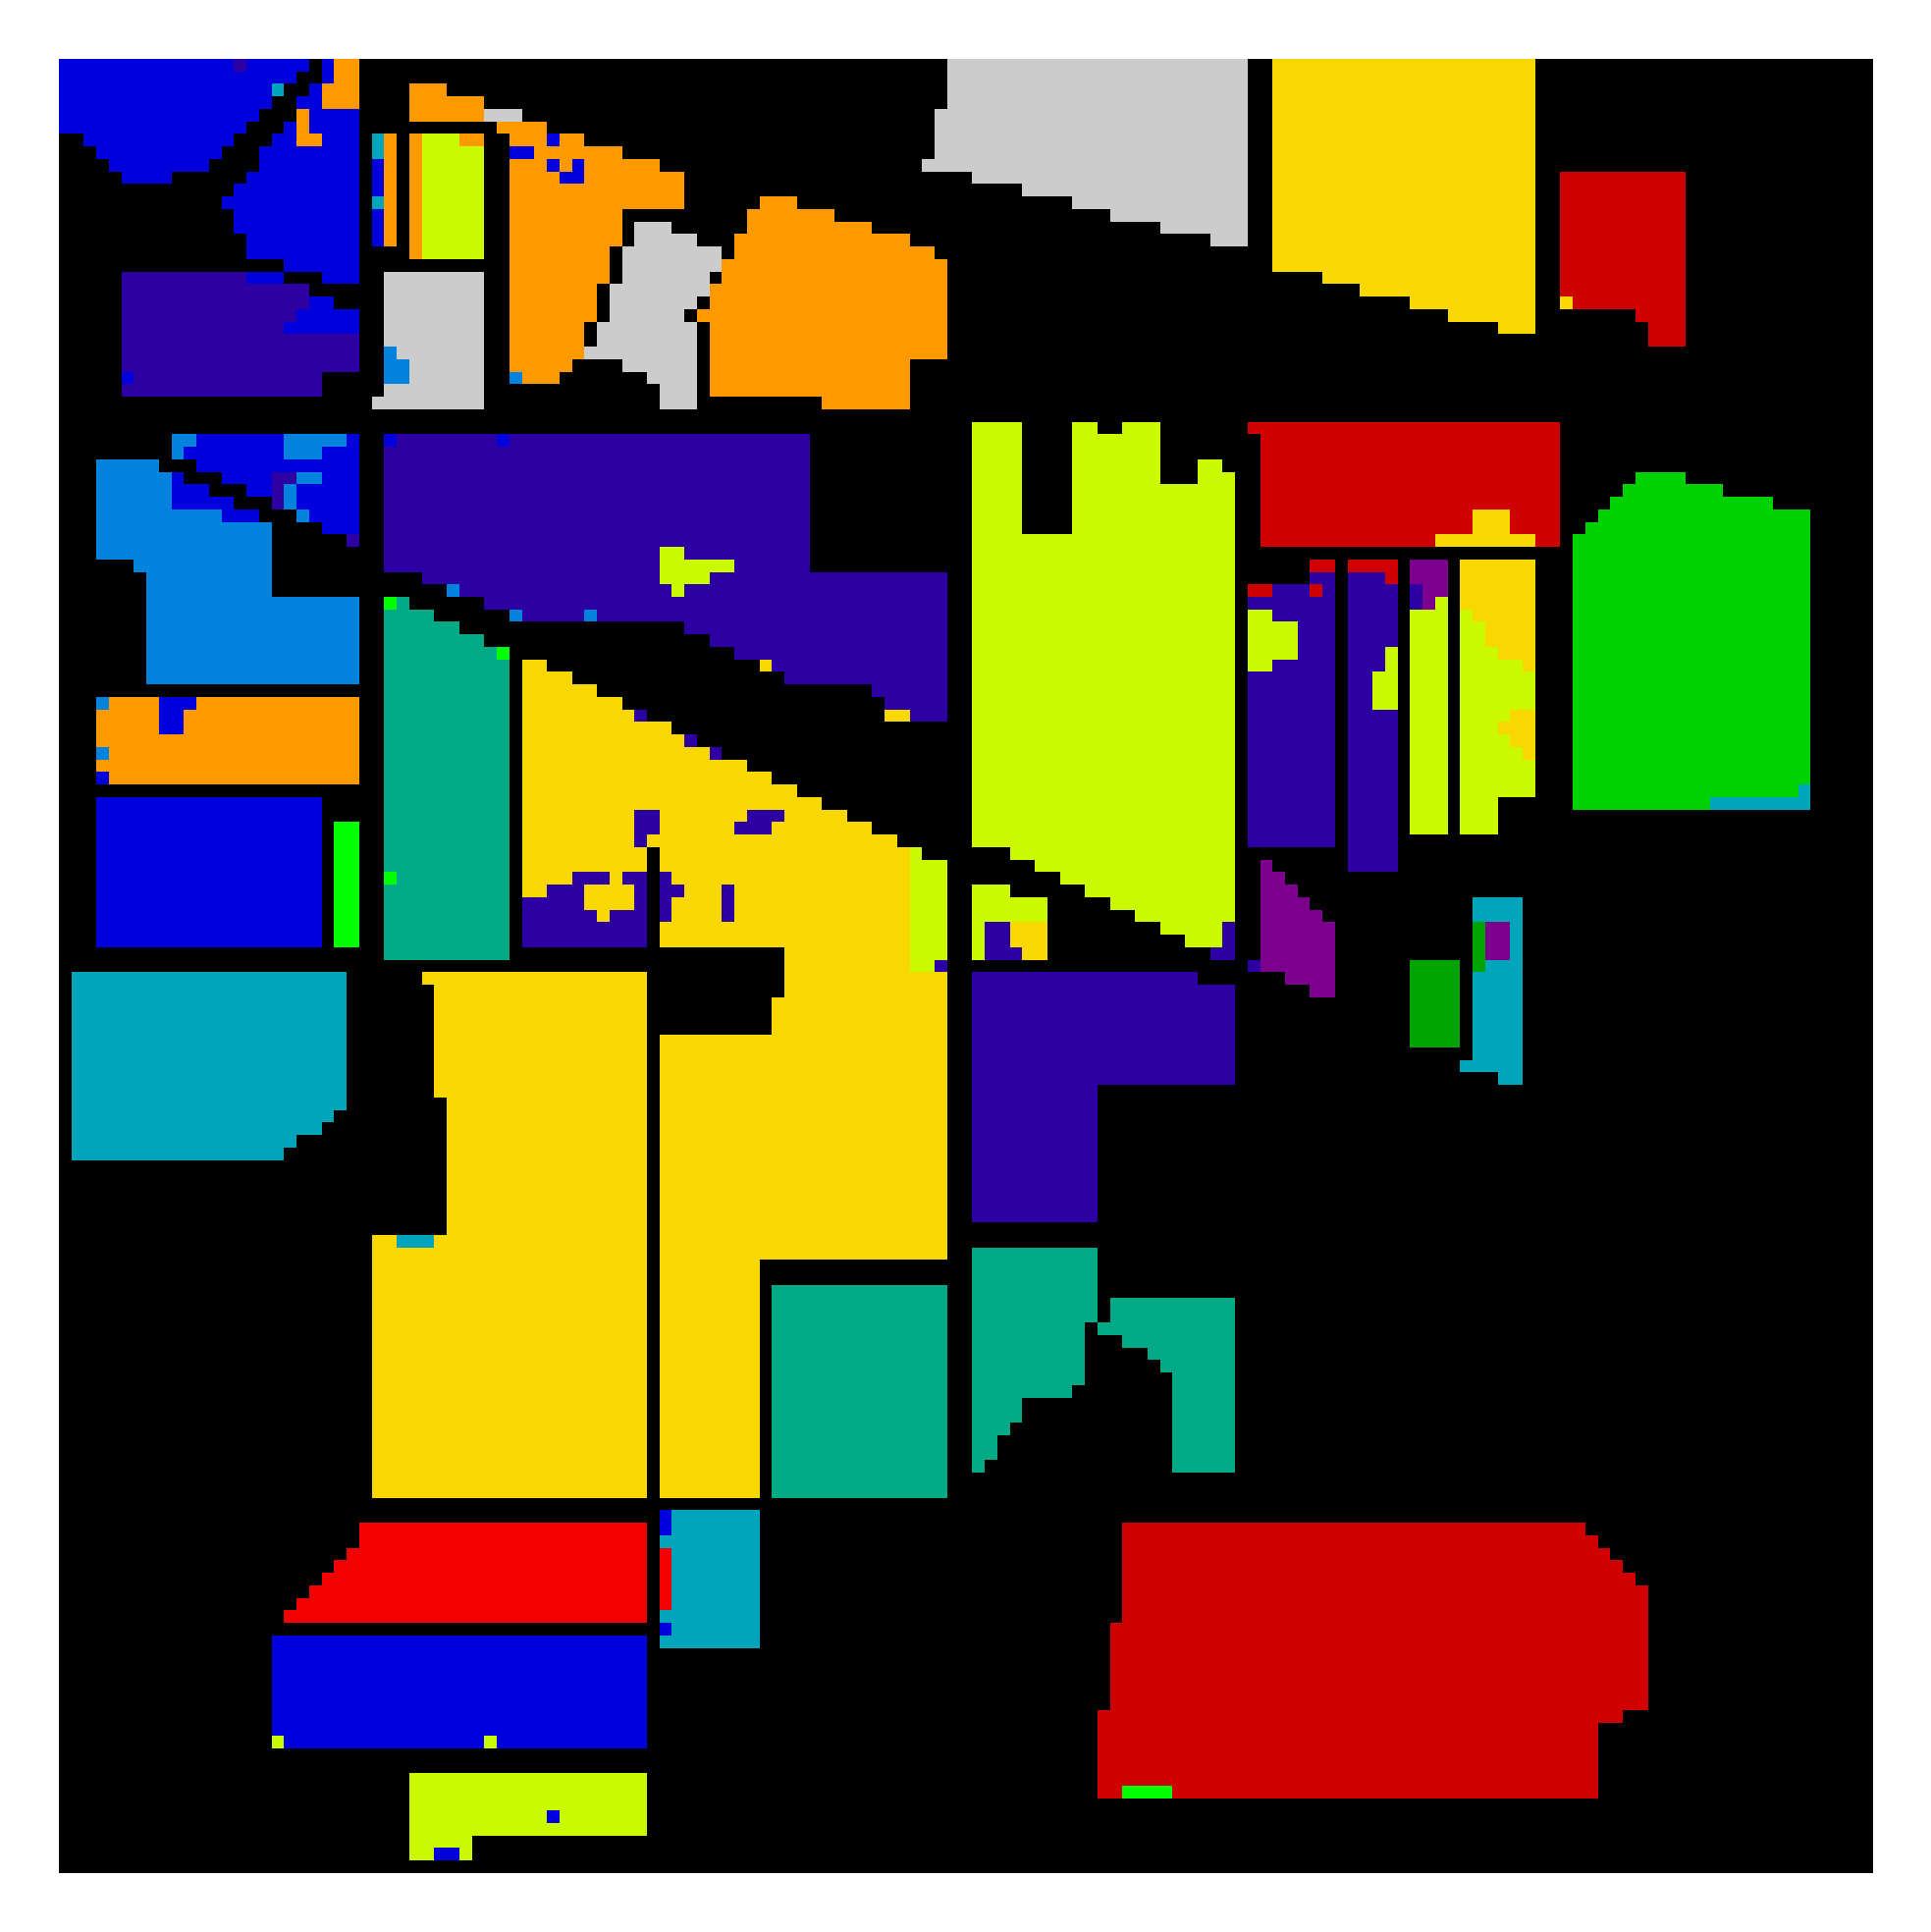
\includegraphics[width=\textwidth]{media/exp3_s3pca_class_map.png}
		\caption{OA = 91.64\%}
	\end{subfigure}
	\caption{Classification maps obtained for the Indian Pines dataset with $T = 30$ training samples per class using (a) Raw data, (b) PCA, (c) SuperPCA, (d) S3-PCA.}
	\label{fig:exp3_maps}
\end{figure}

\section{Novel Settings and Experiments} \label{sec:novel}
In this section, we investigate a few novel settings beyond those explored in the original SuperPCA and S3-PCA framework to better understand the impact of design choices on performance.

First, we examine the effect of the segmentation technique used in SuperPCA and S3-PCA. The original implementation employed ERS applied to the first principal component of the HSI. We compare this approach with two alternatives: (i) using the SLIC algorithm on the first principal component, and (ii) applying ERS directly to the full HSI instead of the projected component.

Next, we explore the choice of similarity measure used to compute reconstruction weights in the S3-PCA method. While the original method is based purely on spectral similarity, we compare this with two alternative strategies: (i) spatial proximity between pixels, and (ii) a combined spatial-spectral similarity measure that balances both aspects. 

\subsubsection{Impact of Segmentation Techniques}

To investigate the influence of segmentation techniques on the performance of SuperPCA and S3-PCA, we perform dimensionality reduction using SuperPCA for various values of the number of superpixels $S \in \{1, 3, 5, 10, 20, 30, 40, 50, 75, 100, 150, 200, 300\}$, followed by SVM classification as outlined previously. We compare three different segmentation approaches.

First, we use ERS on the first principal projection of the HSI, denoted as ERS (PC). This is the setting used by the authors of the original paper \citep{SuperPCA, S3PCA}, who selected ERS due to its high efficiency and favorable performance. The use of the principal component helps speed up the segmentation process.

Second, we employ SLIC, implemented via the \texttt{scikit-image} library. SLIC is one of the most widely used and efficient gradient-based segmentation methods. It is simple to implement and offers reliable results in many standard imaging applications.

Third, we evaluate ERS applied directly on the full HSI, denoted as ERS (HSI). This is feasible because ERS defines edge weights based on the norm in the spectral space, allowing it to leverage the full spectral information. In contrast, SLIC operates in a combined spectral-spatial space, and extending it to the full HSI would involve extremely high-dimensional clustering. This would significantly increase computational costs and potentially degrade performance.

Figure~\ref{fig:exp4} shows the classification results obtained using these three segmentation methods. Figure~\ref{fig:exp4}(a) illustrates the superpixel boundaries generated by ERS (HSI). Although the superpixels appear less regular in shape compared to those produced by SLIC (see Figure \ref{fig:preliminary_results}), they better adhere to object boundaries, which contributes to improved performance. We observe that SLIC and ERS (PC) provide comparable classification accuracies, with no significant advantage of one over the other. However, ERS (HSI) significantly outperforms both methods, leading to an improvement of up to 3.5\% in overall classification accuracy for SuperPCA. This suggests that using the full spectral information in ERS enables the generation of more homogeneous and semantically meaningful superpixels, which facilitates better feature extraction and ultimately improves classification performance.



\begin{figure}[h!]
	\centering
	\begin{subfigure}[b]{0.4\textwidth}
		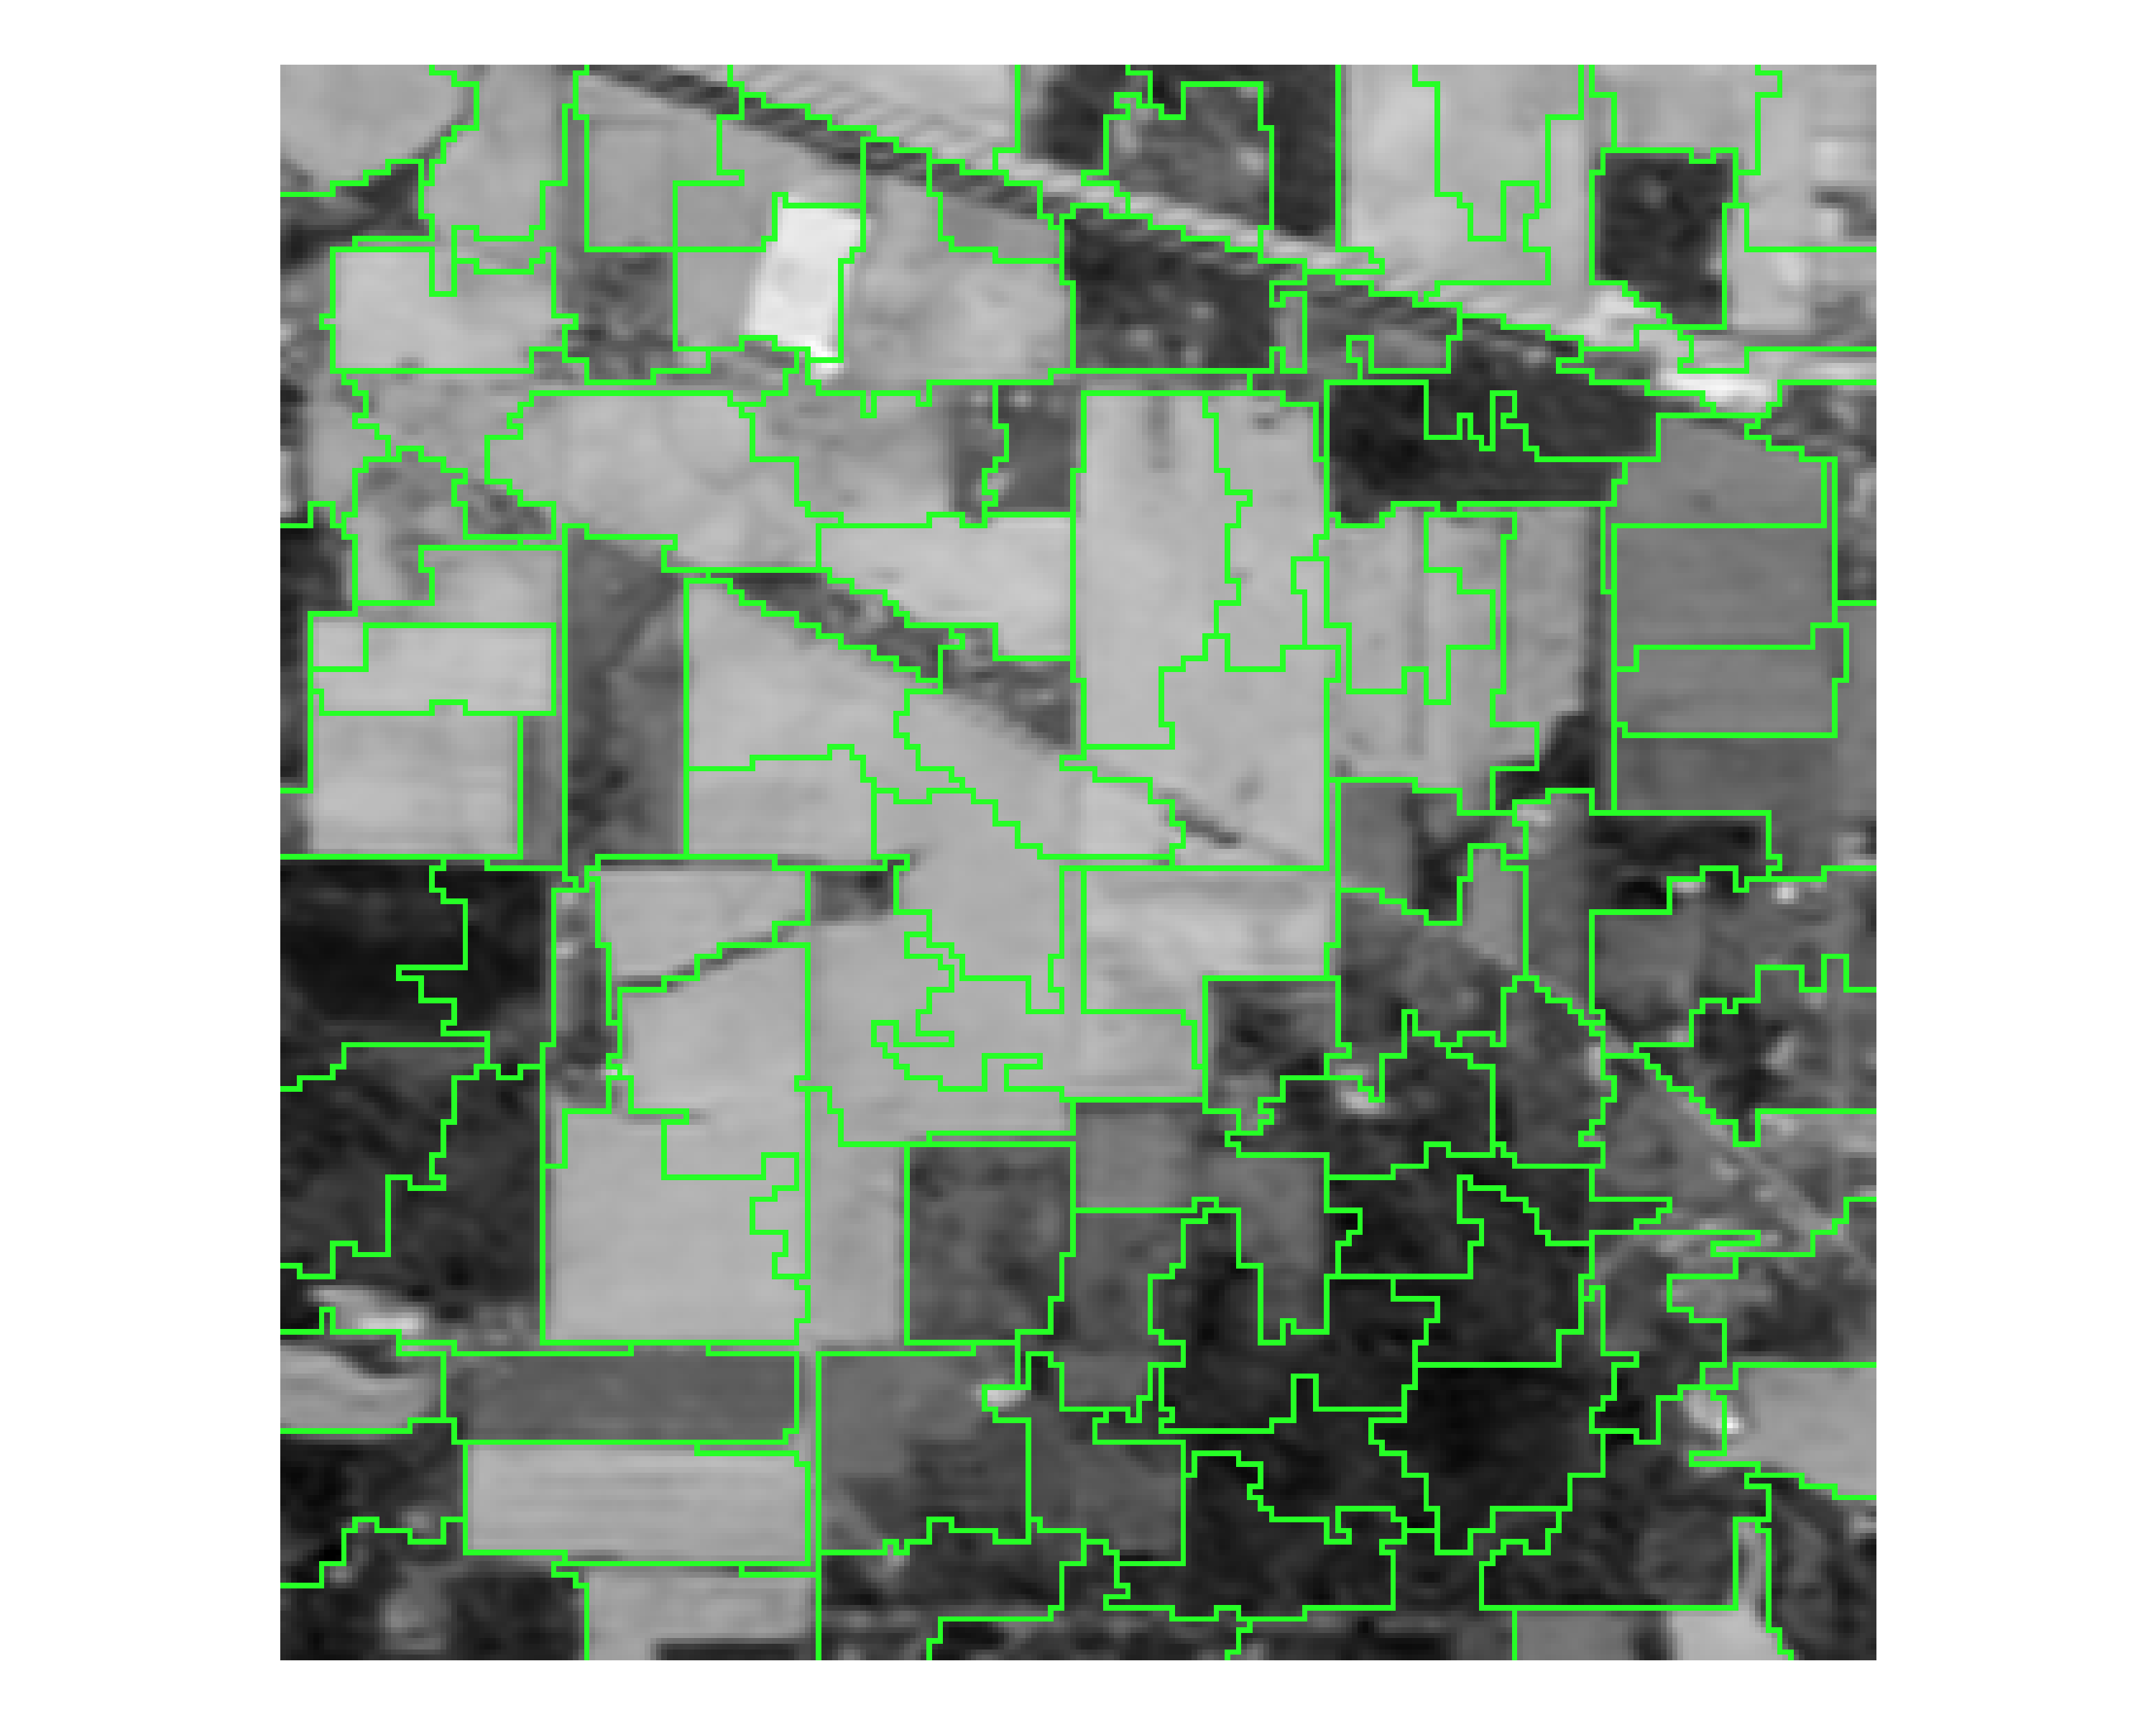
\includegraphics[width=\textwidth]{media/exp4_seg_img.png}
		\caption{}
	\end{subfigure}
	\begin{subfigure}[b]{0.4\textwidth}
			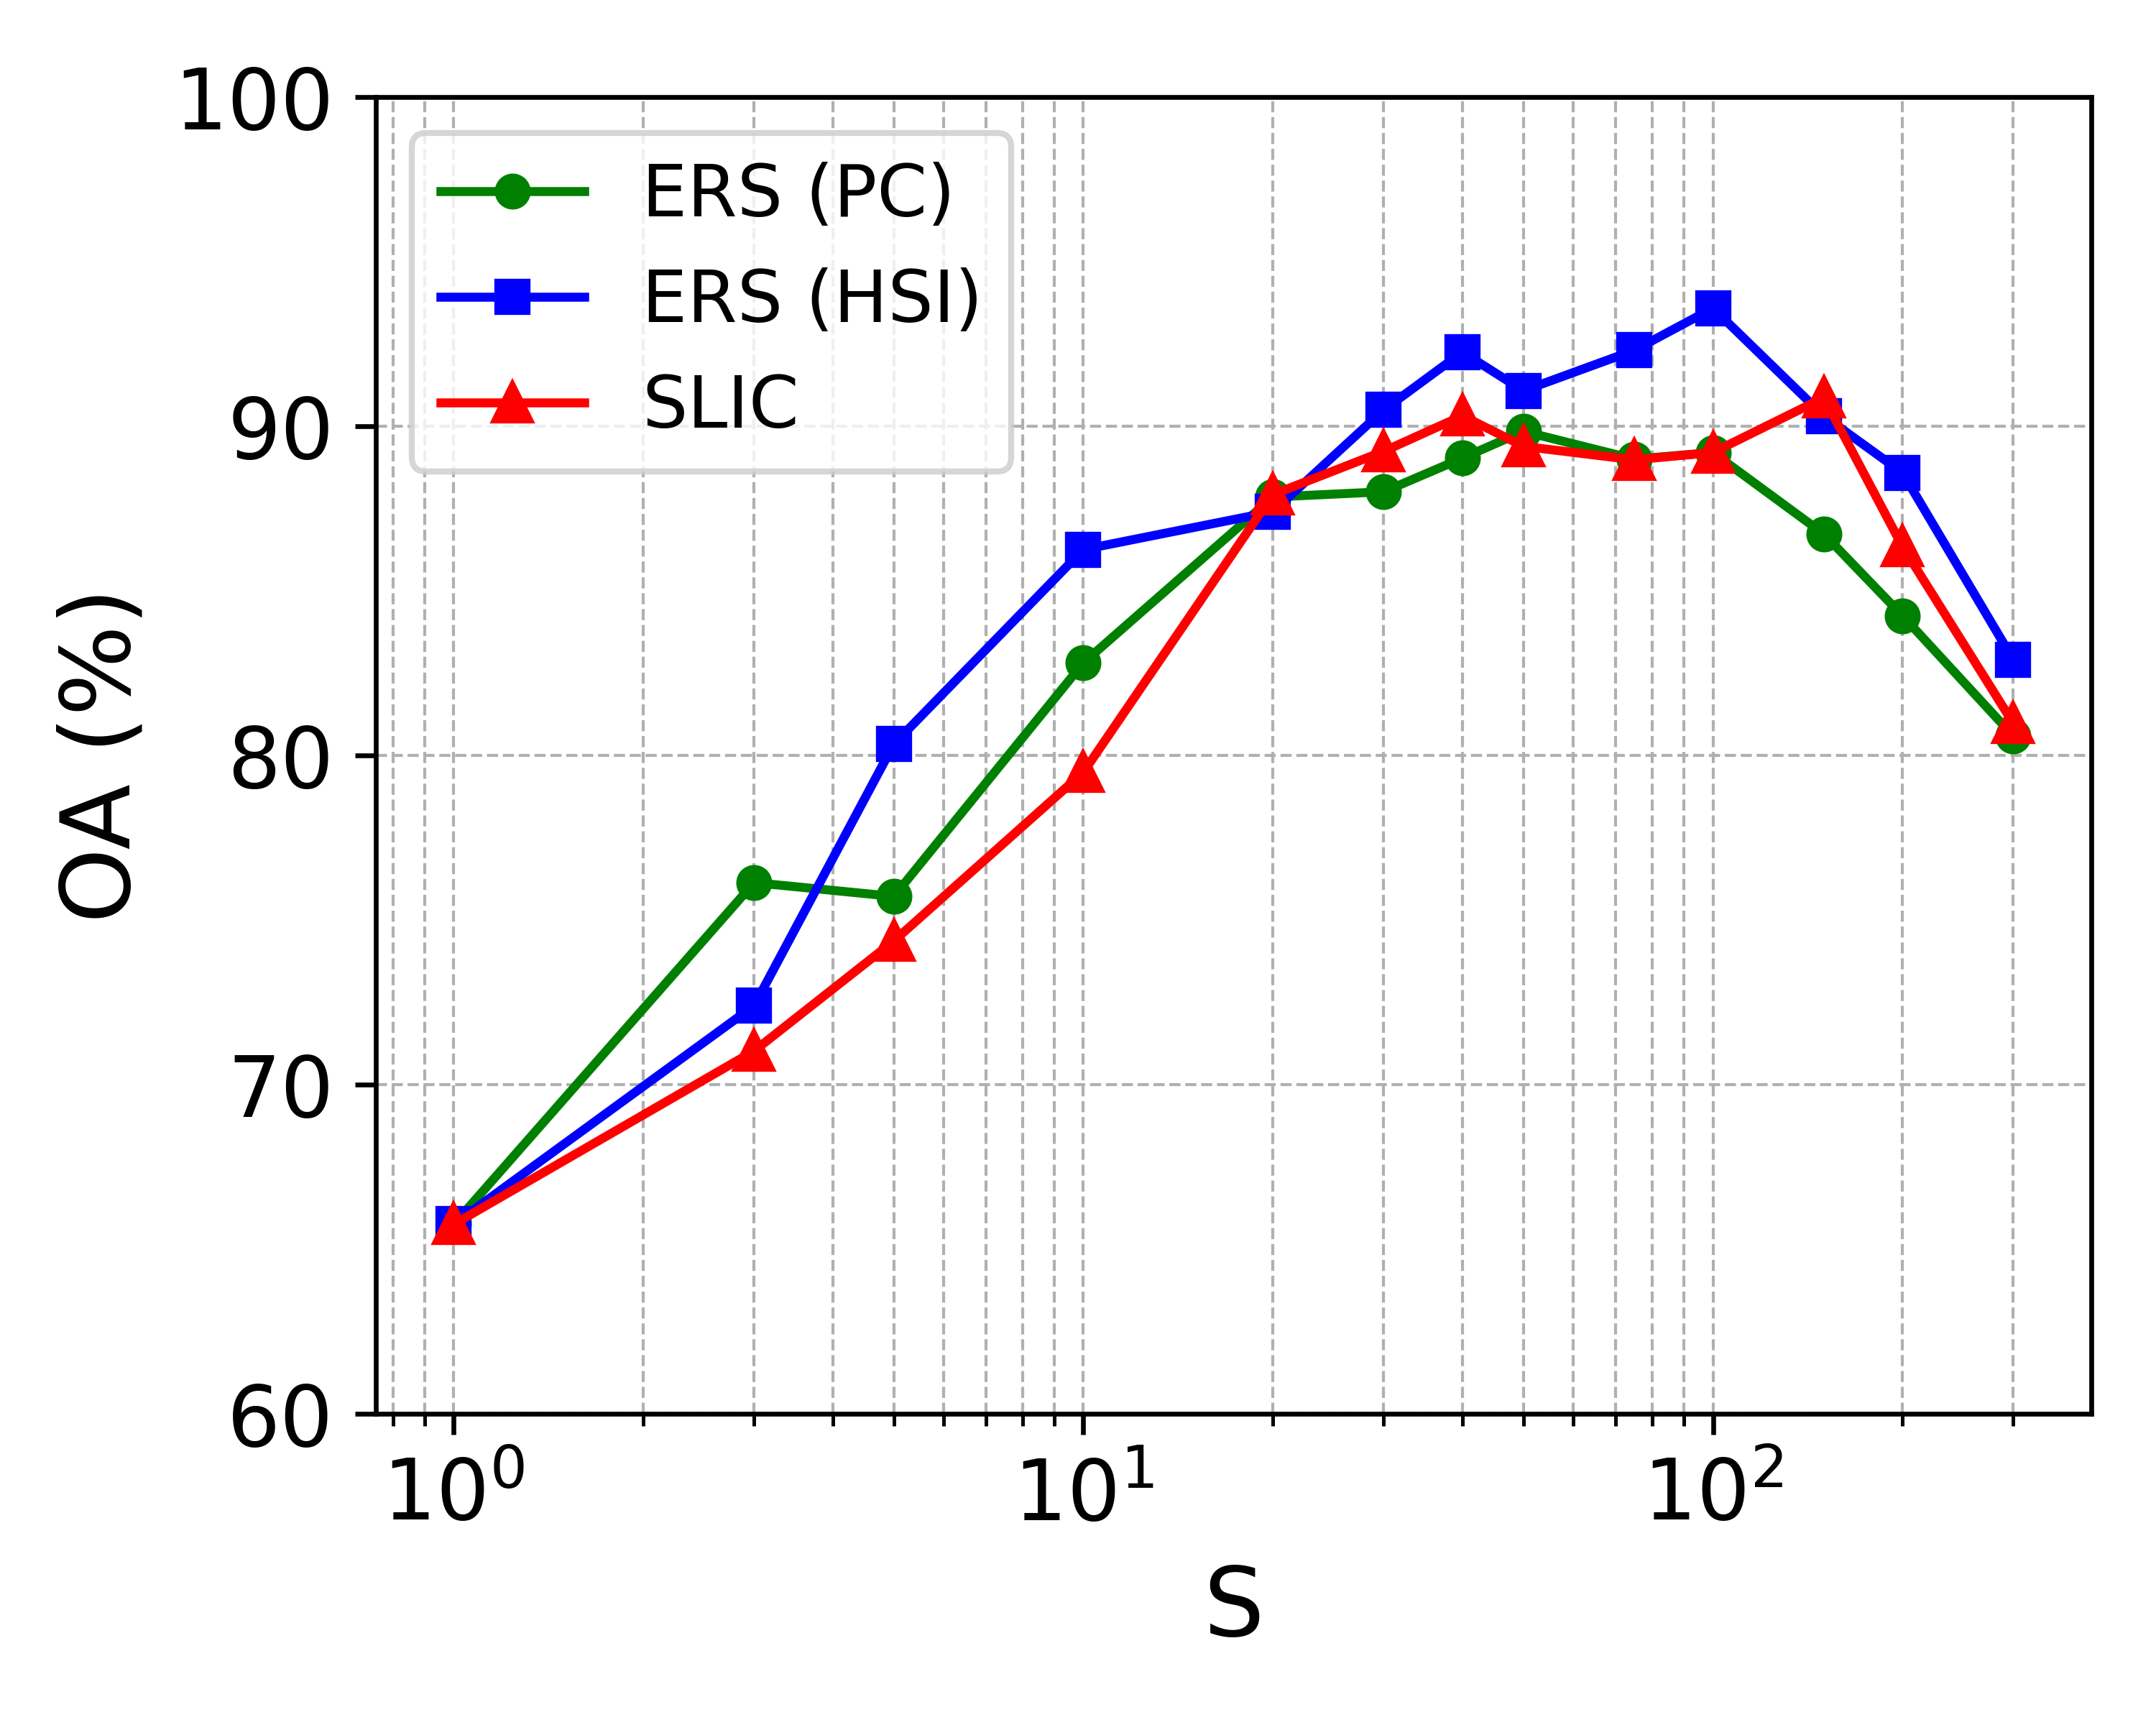
\includegraphics[width=\textwidth]{media/Exp4.png}
		\caption{}
	\end{subfigure}
	\caption{(a) Superpixel boundaries generated using ERS applied to the full hyperspectral image (ERS (HSI)). (b) Overall classification accuracy for different segmentation methods (ERS (PC), SLIC, ERS (HSI)) as a function of the number of superpixels $S$. }
	\label{fig:exp4}
\end{figure}

The only computational overhead introduced by using the full HSI in ERS arises from computing norms in the high-dimensional spectral space instead of in the one-dimensional principal component space. However, this did not result in any noticeable increase in computation time in practice, making ERS (HSI) both effective and computationally feasible.

\subsection{Impact of Reconstruction Criterion in S3-PCA}

To study the influence of the reconstruction criterion in S3-PCA, we perform experiments using ERS (HSI) with $S = 100$ (the optimal value identified in the previous experiment). We vary the number of neighbors $k \in \{5, 7, 9, 11, 13, 15, 17\}$ and evaluate three different reconstruction strategies. The original method proposed by the authors uses Gaussian weights computed using spectral similarity, as described in Section~\ref{sec:s3pca}. In addition to this, we investigate two alternative weighting schemes: one based on spatial proximity, and another based on a combined similarity measure. The combined measure uses the the product of spatial and spectral distances for weighing -- similar to the approach used in the edge weight computation for ERS discussed in Section~\ref{sec:ers}.

Figure~\ref{fig:exp5} presents the results of this comparison. While the inclusion of reconstruction improves the overall classification accuracy compared to standard SuperPCA, we observe that—unlike the case of S3-PCA using ERS (PC) described in Section~\ref{sec:parametertuning} -- there is no clear peak in accuracy with increasing $k$. Furthermore, all three reconstruction methods yield similar overall accuracies, and no consistent or explainable trend emerges. This suggests that when richer superpixels are generated using full spectral information, the choice of reconstruction criterion and the number of neighbors used for reconstruction has a relatively muted impact on final classification performance.

\begin{figure}[h!]
	\centering
	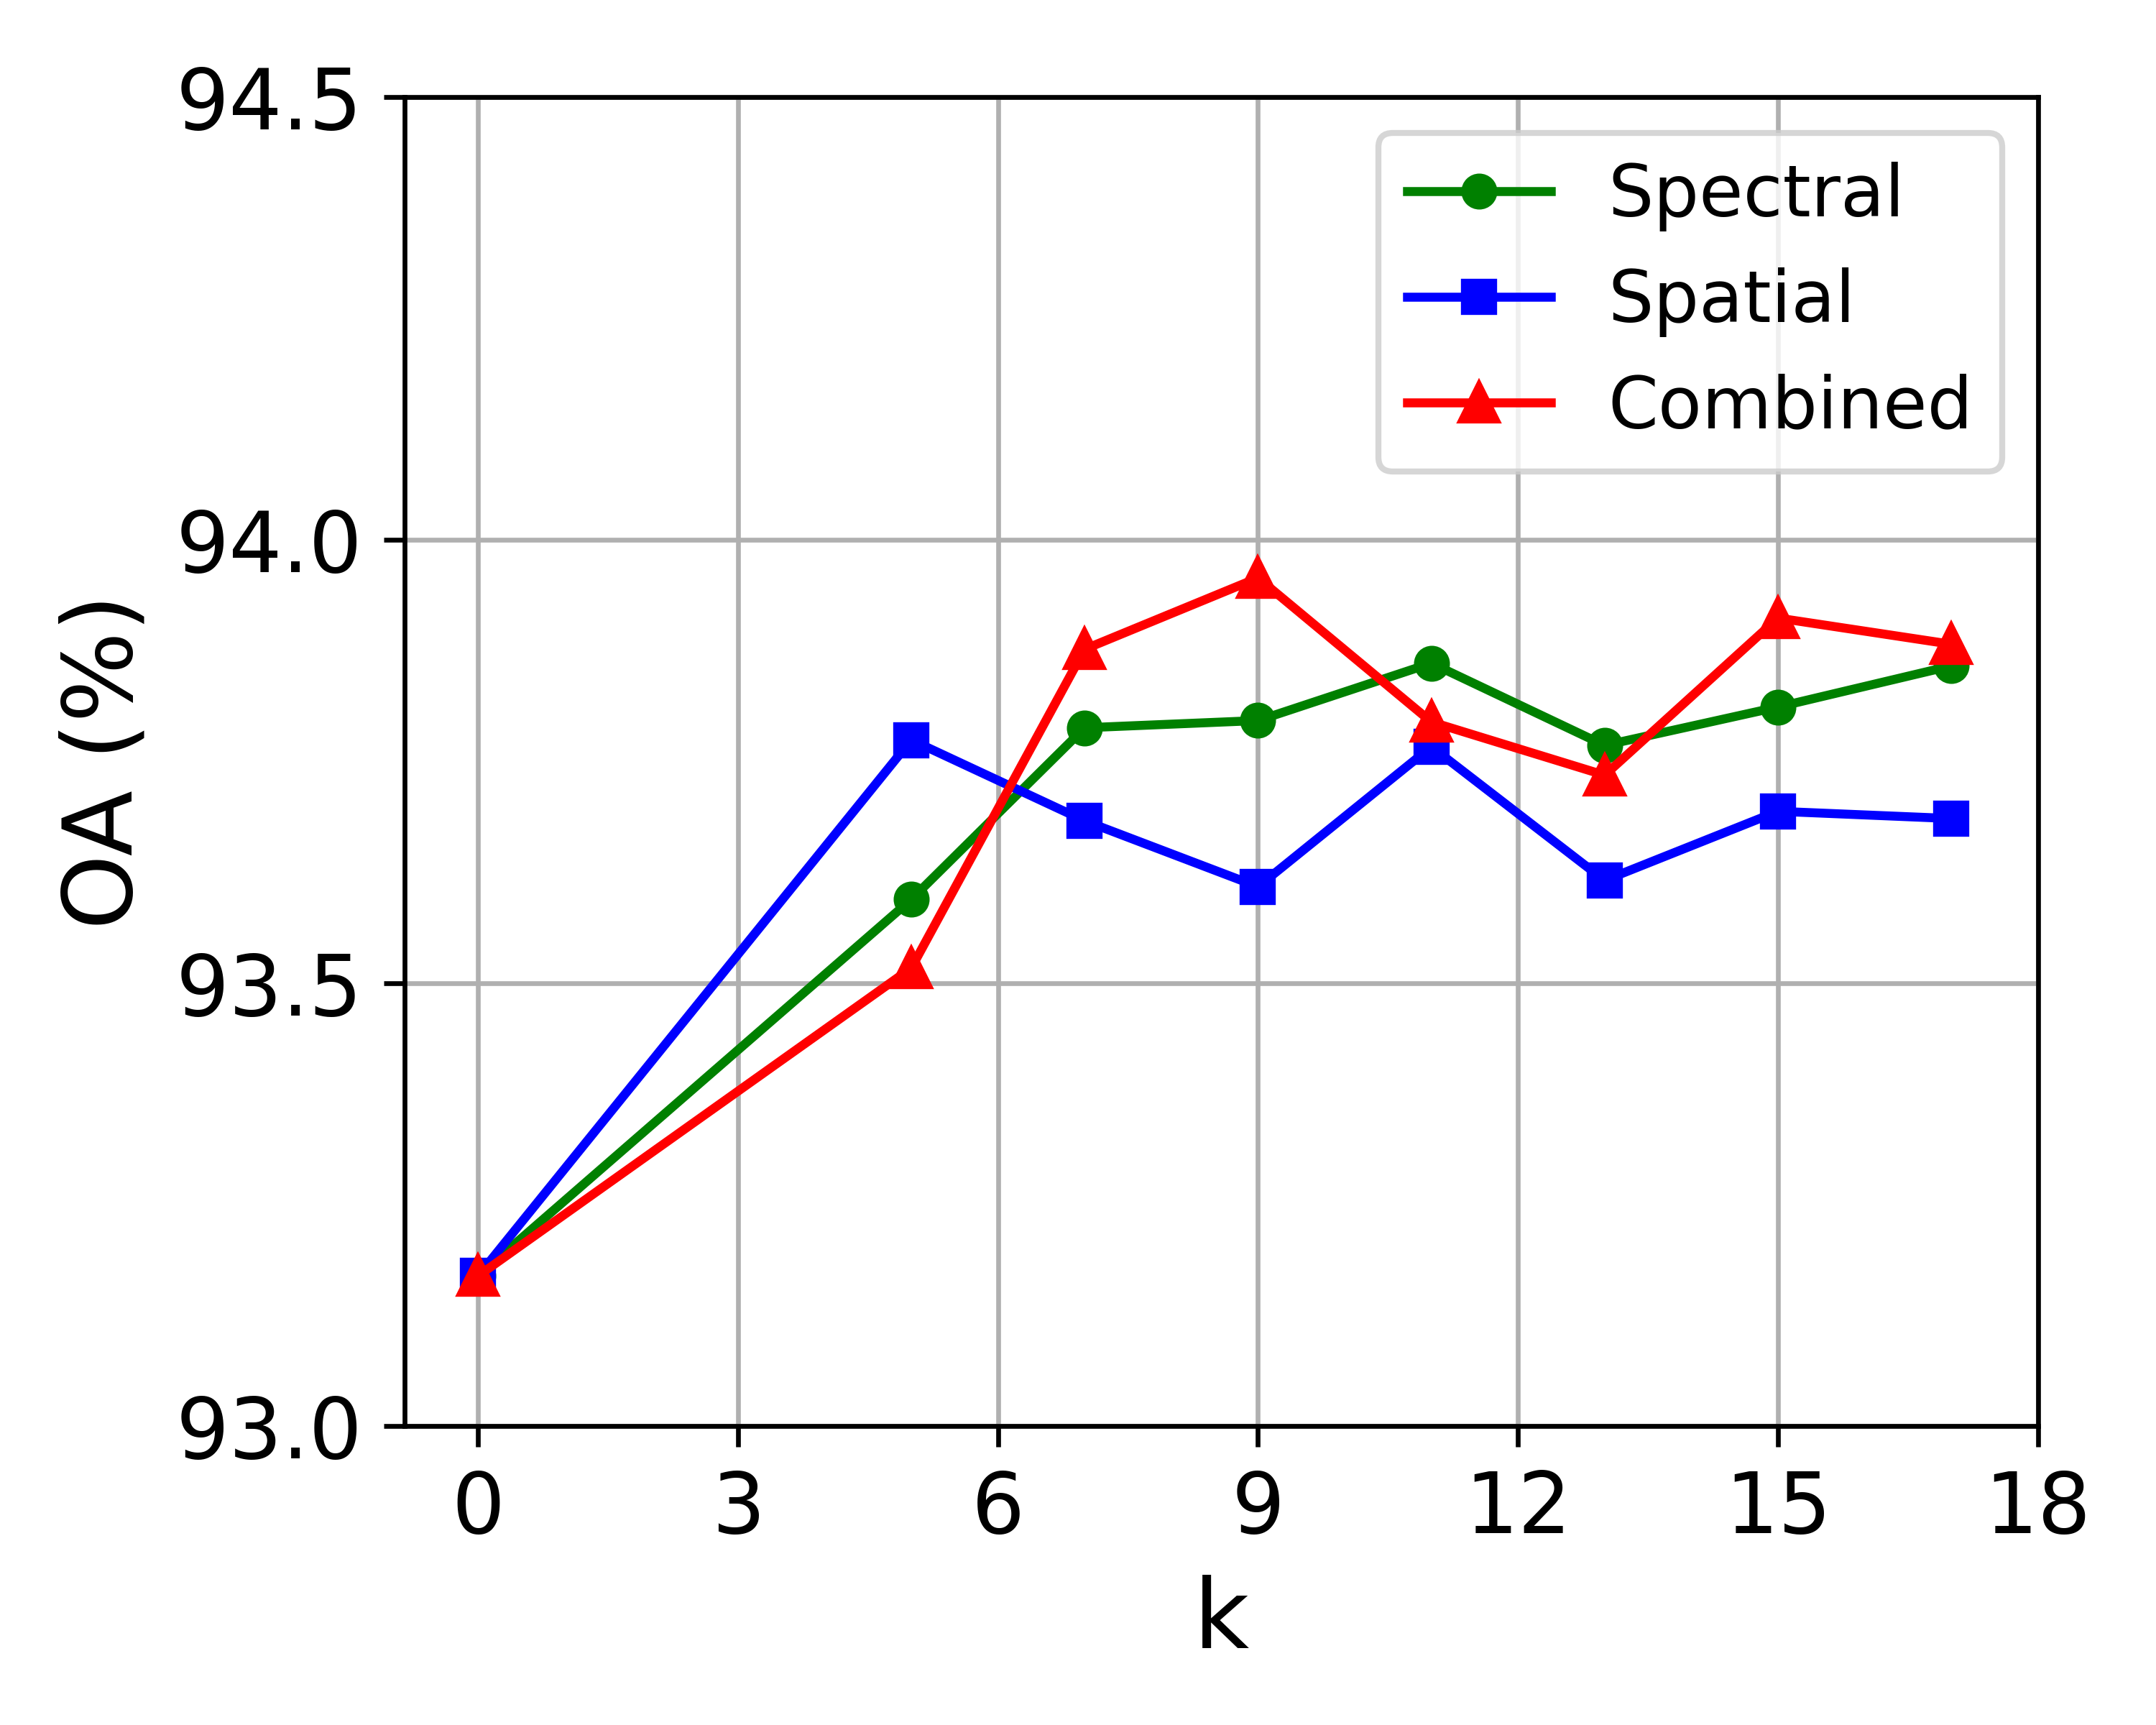
\includegraphics[width=0.4\textwidth]{media/Exp5.png}
	\caption{Overall classification accuracy on the Indian Pines dataset using S3-PCA with different reconstruction methods for varying number of neighbors $k$.}
	\label{fig:exp5}
\end{figure}

\section{Conclusion} \label{sec:conclusion}

Dimensionality reduction (DR) plays a crucial role in hyperspectral image (HSI) analysis, where the high dimensionality of spectral data can lead to the curse of dimensionality and poor classification performance. Traditional methods like Principal Component Analysis (PCA), though widely used, fail to capture spatial context, often resulting in suboptimal representations.

In this project, we studied and evaluated advanced DR techniques -- SuperPCA and S3-PCA -- that incorporate spatial information by segmenting the image into superpixels using techniques such as Entropy Rate Superpixel Segmentation (ERS) and Simple Iterative linear Clustering (SLIC). These methods apply PCA locally within homogeneous clusters to obtain meaningful low-dimensional features. S3-PCA further enhances performance by incorporating both local reconstruction-based denoising and global spatial-spectral features.

We replicated the experiments conducted by the original authors and found that both SuperPCA and S3-PCA significantly outperform PCA in terms of classification accuracy, particularly when their hyperparameters (number of superpixels $S$, number of neighbors $k$) are appropriately tuned.

Beyond the authors' original experiments, we also investigated the impact of segmentation strategies and reconstruction criteria. We observed that using ERS on the full HSI (ERS (HSI)) provides a substantial improvement -- up to 3.5\% in overall accuracy—compared to SLIC or ERS on the first principal component. ERS (HSI) yields more meaningful superpixels by leveraging the full spectral information, resulting in better feature extraction. On the other hand, when ERS (HSI) is used, the reconstruction weighting strategy and the number of neighbors $k$ in S3-PCA have minimal impact on classification accuracy, as long as a sufficient number of neighbors are included.

These findings highlight the importance of the segmentation step in spatial-spectral DR methods. Future work could focus on developing or adapting segmentation algorithms specifically tailored to the characteristics of HSIs, potentially leading to even more discriminative feature extraction and improved classification results.
 
\section{Contributions} \label{sec:contribution}
All work related to this project -- including the implementation, experimentation, and documentation -- was carried out by the sole member.


\bibliographystyle{plain}
\bibliography{references} % Because the file name is demo.bib


\end{document}

